%%%%%%%%%%%%%%%%%%%%%%%%%%%%%%%%%%%%%%%%%%%%%%%%%%%%%%%%%%%%%%%%%%%%%%%%%%%%%%
%
% Main content starts here
%
%%%%%%%%%%%%%%%%%%%%%%%%%%%%%%%%%%%%%%%%%%%%%%%%%%%%%%%%%%%%%%%%%%%%%%%%%%%%%%


\chapter{Introduction}
\label{sec:introduction}

This is a typical human-computer interaction thesis structure for an introduction which is structured in four paragraphs as follows:
% First Paragraph
% CORE MESSAGE OF THIS PARAGRAPH:
\todo{P1.1. What is the large scope of the problem?}
\todo{P1.2. What is the specific problem?}

% Second Paragraph
% CORE MESSAGE OF THIS PARAGRAPH:
\todo{P2.1. The second paragraph should be about what have others been doing}
\todo{P2.2. Why is the problem important? Why was this work carried out?}

% Third Paragraph
% CORE MESSAGE OF THIS PARAGRAPH:
\todo{P3.1. What have you done?}
\todo{P3.2. What is new about your work?}

% Fourth paragraph
% CORE MESSAGE OF THIS PARAGRAPH:
\todo{P4.1. What did you find out? What are the concrete results?}
\todo{P4.2. What are the implications? What does this mean for the bigger picture?}

LaTeX hints are provided in \autoref{chap:latexhints}.

\chapter{Related Work}
\section{Notifications and the Shift to Wearable Audio}
\label{sec:notifications_smartglasses}
Smartphone users receive a large number of notifications. In a study of 203 adolescent smartphone users, Radesky and colleagues report that more than half of the participants received at least 237 notifications per day \cite{URL_23_237NotificationsADay}. Adult users receive fewer raw notifications but interact with their phones at a comparably high rate: a nationally weighted U.S. survey found that adults checked their phones on average 186 times per day in 2025, roughly once every five minutes of waking time \cite{URL_CheckPhone186TimesADay}. Both indicate that mobile devices compete for attention at a rate that exceeds what users can, or want to, act on.\\
Notifications provide valuable awareness of incoming information, yet they are also frequently perceived as disruptive interruptions (ADD PAPERS HERE). \\
In a study of 138 iPhone users, Liao and Sundar \cite{Liao_22_MutedSmartphone} found that vibration-only notifications were the most common configuration (42\%), followed by sound-and-vibration mode (36.2\%), while 8.7\% of participants kept their devices in a fully silent mode. This suggests that users generally wish to remain aware of incoming information, but often avoid continuous auditory alerts in favor of less intrusive notification modalities. Interestingly, users who muted notification sounds did not interact with their phones less. Instead, Liao and Sundar found that soundless notification modes were associated with increased phone-checking behavior and longer usage times, suggesting that reducing auditory cues may increase concerns about missing important information.
Chang and Tang \cite{Chan_15_RingerMode} show that users switch between notification modalities for three primary reasons: to avoid interruption, to prevent their device from disrupting the surrounding environment, and to remain aware of important incoming communication. \\
The increasing adoption of personal audio technologies, such as wireless earbuds and audio-enabled smart glasses, partially alleviates the second concern by enabling notifications to be delivered privately to the wearer. This not only reduces the risk of disturbing nearby individuals but also enables the use of richer auditory notification modalities, such as spoken sender names or message content, that would be socially inappropriate when broadcast through loudspeakers. Consequently, the challenge shifts from deciding whether a notification should be audible to determining how much information should be conveyed and when it should be presented so that users remain aware of important communication without being unnecessarily interrupted. This question becomes particularly relevant with smart glasses. They can be worn continuously and unobtrusively throughout the day and create opportunities to deliver auditory notifications in situations where users would not typically wear headphones or earbuds. Consequently, understanding when and how auditory information should be presented becomes a critical challenge for future wearable computing systems.

\section{Auditory Displays}
Auditory Displays can be defined as ''the use of sound to communicate information about the state of a computing device to a user'' \cite{Mcgookin_04_ExplainAuditoryDisplaysWiki}. The First International Conference on Auditory Displays (ICAD 1992, Santa Fe) launched the field, with proceedings published as the seminal volume \textit{Auditory Display: Sonification, Audification, and Auditory Interfaces} \cite{Kramer_94_AuditoryDisplay}.\\
\textbf{\glspl{type}} define different ways of representing information through sound and are, in this thesis, simply defined as \textbf{\glspl{type}}:

\textbf{Auditory Icons} have first been introduced by Gaver in 1986 \cite{Gaver_86_IntroducedAuditoryIcons} and can be defined as ''everyday sounds mapped to computer events by analogy with everyday sound-producing events'' \cite{Gaver_93_AuditoryIcons},
thereby utilizing users' prior knowledge and associations with sound sources and causes \cite{Dingler_08_AuditoryDisplayTypesOverview}.\\
Gaver instantiated this idea in the \textit{SonicFinder} \cite{Gaver_89_SonicFinderUsingIcons}, a prototype interface that adds sound to a normal desktop UI.
For example, selecting a file produces a tapping sound, where the file size determines the pitch. Dragging a file triggers a scraping sound, while dropping it into the trash produces a crashing sound.\\
Early Auditory Displays leaned heavily on Auditory Icons and literal everyday sounds. 
Modern systems moved away from that, but Auditory Icons are still prevalent (e.g., camera shutter sound when taking a photo, or keyboard typing sound on touchscreens). Systems such as Windows have explicitly shifted toward subtle synthetic tones, deliberately avoiding realistic everyday environmental sounds \cite{URL_WindowsSounds}. 
For instance, the \textit{Sonification Handbook} highlights a core practical limitation of literal icons in digital interfaces: ``Physical windows in the real world open slowly but windows in a graphical user interface typically zoom in or pop out quickly. This meant that using real sounds of a window’s opening or closing would be inappropriate'' \cite{Hermann_11_SonificationHandbook}.

\textbf{Earcons} were first introduced in 1989 by Blattner et al. \cite{Blattner_89_EarconsAndIcons}. In contrast to auditory icons, earcons are abstract synthetic sounds that are not directly associated with real-world sound sources, but are often designed to be easily distinguishable and memorable, suited when there is no intuitive sound to represent the data \cite{Mcgookin_04_ExplainAuditoryDisplaysWiki}.
Because of the lacking inherent relationship between sound and meaning, earcons require users to learn how they are linked with events \cite{Hermann_11_SonificationHandbook}. Typical examples include the short two-tone sound that signals the activation of a voice assistant or the descending three-note pitch-and-volume pattern used as a low-battery warnings. In both cases the sounds are purely synthetic and abstract, with no direct real-world source, yet users quickly learn the mapping through repeated exposure or onboarding.
While auditory icons and earcons are frequently presented as distinct categories, the boundary between them is not strictly binary. Earcons can be designed to be more intuitive by incorporating metaphorical elements drawn from real-world events, thereby blending influences from auditory icons.

\textbf{Speech} Displays use natural or synthetic spoken language to convey information directly, often realised through \gls{tts} systems. Contemporary examples include screen readers (e.g., Apple’s VoiceOver) or voice assistants (e.g., Google Assistant: ''You have two new messages from Anna.'').\\ 
\textbf{Spearcons} (Speech-Based Earcons) were first introduced in 2006 by Walker et al. \cite{Walker_06_SpearconsInMenus}, and are created by speeding up vocal audio to the point that it is no longer comprehensible as speech. They are currently more common in research and specialized accessibility prototypes than in mass-market consumer devices. Spearcons are often explored in gesture interactions like in in-vehicle menu navigation \cite{Tabbarah_23_InCarMenuNavAuditorySpearcons} where auditory displays must present accurate, simple feedback to reduce the driver’s cognitive demand \cite{Cooper_15_CognitiveDemandVehicleSpearcon}. Speech and Spearcons do not need to be learned due to their intrinsic nature of conveying the underlying information in a medium the recipient already understands, thereby making them appropriate in accurate, precise-demanding situations achieving high recognition accuracy with virtually no training, often outperforming earcons \cite{Walker_06_SpearconsInMenus}.
However, they can be difficult to perceive in noisy verbal environments and have a strong potential to interfere with concurrent speech communication as the spoken cues compete directly with other voices \cite{Davidson_19_SpearconsInterfereVoice}. Speech-based displays can also introduce privacy risks (e.g., sensitive medical information such as “low blood pressure” being announced aloud in public) and language barriers for non-native speakers or multilingual users who show reduced comprehension especially under noisy conditions \cite{Skoe_19_BilingualismHarderSpeechUnderstandingNoiseEnv}. %\hl{var0, issues with speech}.
Further speech-based variations can be conceptualized and include for example spindices, which use accelerated initial sounds and could be applied for rapid alphabetical list navigation. Auditory emoticons, which rely on non-verbal human sounds like laughter to express emotion, or spemoticons, which modulate meaningless, TTS-synthesized vocalizations to convey more affective states \cite{Csapo_13_ModernAuditoryDisplayTypesOverview}.


\textbf{Hybrid} sounds can be created by combining different \glspl{type}. For example, an earcon can be paired with speech so that an abstract signal is reinforced with verbal information. This kind of combination draws on the strengths of each type, possibly allowing one to compensate for the limitations of the other \cite{Dingler_08_AuditoryDisplayTypesOverview}. Contemprary examples can often be found in voice assistants (e.g., Google Assistant) that often produce a short, abstract earcon (a brief tone signaling readiness), followed immediately by speech output, such as ''How can I help you?''. In this case, the earcon provides fast, low-effort recognition of the system state, while the speech delivers precise, semantic information.

High-level summaries and taxonomies of the full range of \glspl{type} can be found in the comprehensive survey by Csapó et al. \cite{Csapo_13_ModernAuditoryDisplayTypesOverview}, which systematically reviews auditory representations in human-machine interfaces, and in the more recent systematic review and meta-analysis by Nees and Liebman \cite{Nees_23_AuditoryDisplayTypesHCI}, which focuses specifically on brief audio alerts and empirically compares auditory icons, earcons, spearcons, speech, and hybrid variants across performance, workload, and preference metrics.\\

\textit{$\rightarrow$ Different \glspl{type} involve distinct trade-offs: auditory icons are intuitive but limited by prior real-world associations and digital application space, earcons are flexible but require training, and speech provides semantic clarity but suffers from privacy concerns and masking in noisy verbal environments. Hybrid sounds can combine the strengths of these different \glspl{type}. Ultimately, this highlights that selecting an appropriate \gls{type} is a complex design problem that heavily depends and changes based on the user's current situation, needs, and experience.}

\subsection{Sonification, Psychoacoustics, \& Auditory Display Presentation Strategies}
state here things about timbre, pitch, e.g.. effects on humans liek energectics and infromational masking,
and also how auditory displays might be altered to facilitate this (e.g. delay)

\section{\gls{aui}}
''An adaptive user interface is a software artifact that improves its ability to interact with a user by constructing a user model based on partial experience with that user.'' \cite{Langley_09_AdaptiveInterfacesDefinition}.
This definition shows that an \gls{aui} doesn’t work on its own but is made to interact with a person. To be truly adaptive, the system has to get better at working with that person over time. Simply remembering past interactions isn’t enough. Instead, it should learn patterns from those experiences and use them to handle new interactions more effectively.\\
Each user has different habits, preferences, and ways of working. An \gls{iui} like an \gls{aui} takes these into consideration and provides personalized interaction methods. \glspl{iui} can filter out irrelevant information thereby reducing cognitive load. They can see what tasks the user wants to accomplish, understand the context, recognize the users' attempt, and aid the execution of their task \cite{Alvarez_09_IUIChallengesBenefits}.
However, ''adaptive automation should not be regarded as a panacea for all the problems that confront the user. The designer must first determine whether the user really needs an adaptive system.'' \cite{Roth_02_DownsidesAUI}.\\
While early \glspl{aui} focused mainly on desktop or web GUIs, recent systematic reviews show that adaptive interfaces have expanded into a wide range of domains, including mobile and web platforms, automotive systems, IoT/smart environments, education, healthcare, and immersive evironments such as \gls{ar}, \gls{vr}, and \gls{mr} \cite{Kristic_25_AUIOverviewAndApplications, Kourtesis_24_XRApplicationAUI}.
To enable this adaptiveness and intelligence, the system fundamentally requires continuous information regarding the user and potentionally their surroundings. While traditional computing platforms can rely on standard interaction logs to infer user models, sensor-rich and immersive systems, equipped with visual, auditory, and other tracking sensors, benefit for designing \glspl{aui}. These multimodal capabilities provide the system with real-time access to the user's physical environment, attention, and underlying intentions, allowing the interface to dynamically adapt to their immediate context \cite{Evangel_22_AdaptiveInXR, Suzuki_23_XRandAIDirections}.
\subsection{\gls{aaui}}
Building upon the principles of adaptive systems, I define an \gls{aaui} as a interface that dynamically adapts its auditory output to the user's current context, or utilizes the user's acoustic environment to drive adaptations of the system.
In the scope of this thesis, an \gls{aaui} encompasses two dimensions:\\
The system's ability to intelligently modulate its audio-based feedback based on the user's state (determined via auditory or non-auditory modalities), and its capacity to actively sense and respond to the real-time acoustic environment surrounding the user.\\
\subsubsection{\gls{aaui}: Notifications}
Similar directions as this thesis' \textit{SonoAdapt}, are for example researched via Wang et al.'s \textit{MARingBA} \cite{Wang_24_Maringba}, which blends ringtones into background music to modulate how noticable they are. They achieve this, by using \gls{mir} to derive the musics' quantifiable features (e.g., Key, Tempo, Pitch) and adapt the notifications' to it. With this, \textit{MARingBA} highlights most systems present non-adaptive approaches in regards to the environmental soundscape: ''[...] audio notifcations are typically delivered in one of two ways: either they mute whatever the user is listening to or they are directly overlaid.''. However, with this the following issues arise: albeit the muting ensures that the notification is noticed, it fully interrupts the listening experience, and with the notification overlaying the music, the notification becomes potentionally unnoticeable and the two sound sources might sound unpleasant together. %\hl{var23->the potential salience and disruptiveness of the notification depends on the user current auditory soundscape} 
\textit{MARingBA} requires pre-processing of the song which takes approximately one minute highlighting the need for better future \gls{mir} approaches. %\hl{var1->quicker/better understand the user auditory context}
They also state that \textit{sheduling} (i.e. timing and delaying the notification in focus) can be further explored as way of making this system more flexible for adaptiveness. %\hl{var2->explore timeleiny parameters as a auditory display type}
Wang et al. also proposed a system that synthesizes a spoken notification as a singing voice with a melody that is then fitted by temporaly replacing the original vocals of the background music \cite{Wang_24_MusicAwareAssist}. Next to issues with their used \gls{svs} and their solution of using manual \gls{tts} and pitch-shifting, which made the singing ''robotic'' sounding, they highlight one important issue, which was also discussed in their \textit{MARingBA} system: Because of the notifications seamlessly harmonizing within the music, users sometimes didn't realize a notification had started or appeared, requiring extra cognitive effort to decipher the message or recognize the notification. %\hl{var3->baesd on the auditory soudnscpae, a sound notification might be overheard, also in adaptive systems when adapted wrongly, need to balance this}. 
Moreover, long or complex notifications (e.g., emails) disrupted the musical flow and trying to stretch or compress too many syllables into a short musical phrase destroyed the natural rhythm of speech. %\hl{var3->balance intrusiveness/salience}.
To facilitate this, Wang et al.'s \textit{MARingBA} had musicians create parameter presets for three specific scenarios: Low Urgency (e.g., a weather update), Medium Urgency (e.g., a meeting in two hours), and High Urgency (e.g., a boss needing an immediate reply). Users overwhelmingly preferred the "Medium Urgency" setting. This setting applied some musical adaptation (like matching the beat and key so it wasn't harsh) but retained enough contrast (salience) so the user didn't have to  expend extra cognitive effort to realize a notification was happening. %\hl{var4->need to deduce correlation between set urgency and user expected/accepted form of covneying this auditorily}.
Addressing the impact of external soundscapes, Ahmetovic et al. \cite{Ahmetovic_23_AdaptiveScreenReader} introduced an adaptive screen reader that dynamically counteracts environmental noise using real-time audio equalization, volume, and speech rate adjustments. Their findings demonstrate that combining these methods significantly enhances speech clarity for blind users in noisy settings, such as crowds or traffic, without sacrificing their awareness of critical surrounding sounds. %\hl{var->understood calrity of speech suffers from env noise}
Streefkerk et al. \cite{Streefker_07_PolicePatrolMessagePriorityBasedOnContext} present an early context-aware notification system for mobile police officers, adapting salience and information density based on the messages' priority and user workload. Their evaluation shows improved task performance and reduced interruption, but relies on experimentally induced context and simple rule-based mappings. Building on this, Streefkerk et al. \cite{Streefkerk_12_PolicePatrolAdaptiveNotifications} extend the approach by incorporating user activity and adapting notification timing and presentation (e.g., full message, indicator, postponement). However, both systems remain limited by manually defined context models and discrete adaptation strategies without real-time multimodal sensing or audio adaptation. Yet, they highlight that ''the priority of the notification should be considered with respect to the priority of the ongoing task''.  %\hl{var11->lack of real-time multimodal context inference (e.g., auditory/visual scene understanding)} \hl{var12->limited adaptation space focused on discrete notification styles rather than continuous auditory parameterization} \hl{var13->no modeling of perceptual audio properties such as salience or masking in dynamic soundscapes} \hl{var14->highlighting that we need to infer the priority of the notification with respect to the ongoing task. Right now It is predefined by the experimenters/scenario designers}
\\

\textit{$\rightarrow$ While approaches have been made to make auditory notifications and auditory content adaptive to the user's environment, current implementations face several limitations. Existing systems demonstrate that adjusting acoustic parameters or harmonizing sounds with the background can reduce disruption and improve clarity. However, they frequently rely on slow processing, manually pre-defined context models, and notification just adapting within its range of pre-defined types and scenarios (e.g., music). Moreover, by lacking real-time context inference, these systems cannot dynamically assess and adapt a notification's significance relative to the user's ongoing task. With this they leave notifications at risk of either being lost in dynamic environmental noise or becoming overly disruptive. A fundamental gap remains in continuously balancing recognizability and intrusiveness across complex, varying contexts.}

\subsubsection{\gls{aaui}: Hearing}
\label{sec:aaui_hearing}
A lot of research focuses on making a users auditory experience with his environment more personalized and adaptive \cite{Haas_20_TargetAudioPersonalSoundscapeHearables}. The technological approaches thereby often revolve around understanding or registering the auditory soundscape and scene which is further explored in Section \ref{sec:auditory_scene_understanding}.
Hearable consumer devices like headsets, and earbuds, often incoorperate \gls{anc} and acoustic transparency.
\gls{anc} is a well-researched problem where microphones are used to capture the soundscape and an anti-noise signal is then transmitted back to cancel all recorded external sounds and noise in virtual real-time \cite{Shen_18_ANC}.\\
\textit{Semantic hearing} leverages the idea behind noise-cancelling earphones to suppress all ambient sound, then applies semantic reasoning to interpret and reconstruct meaningful acoustic scenes in real time. Veluri et al. explored semantic hearing in \cite{Veluri_23_SemanticHearing}, where users can select specific sound categories (e.g., sirens, birds, speech) to hear while blocking out  other interfering background noise, all while preserving the spatial directionality (binaural cues) of the target sounds. In \cite{Veluri_24_LookOnceToHearTargetSpeech} by Veluri et al. they introduce a system where a user simply looks at a specific target speaker in a potentially noisy/crowded room for a few seconds. The hearable captures the speaker's acoustic traits and then selectively extracts only that speaker's voice, even if the user looks away or moves around. Both papers rely on explicit user input. Either the user must manually select "birds" or "sirens" on an app, or the user must press a button and look at a speaker to enroll them. %\hl{var5-> SonoAdapt aims to infer the user's task and situation autonomously using real-time scene understanding. You are moving the field from manual acoustic selection to intelligent, context-aware adaptation. (SonoAdapt) doesn't just filter the world; it augments it safely. While recent advances allow for the semantic filtering of real-world soundscapes (Veluri et al., 2023), there is a critical gap in how we dynamically introduce synthetic Auditory Displays into these complex, filtered, or unfiltered environments without overwhelming the user}.
\textit{MoXaRt} by Xu et al. \cite{Xu_26_TargetAudioXR} introduced an \gls{mr} system that uses a combination of audio and visual data to separate concurrent sound sources in real-time. It visually identifies objects making noise (e.g., detecting faces for speech, or instruments for music) and uses those visual anchors to feed an audio-separation neural network. This allows users to visually select a specific person or instrument in their environment and independently adjust their volume. %\hl{var6: ou can cite MoXaRt to state that while multimodal scene understanding is now successfully being used to manipulate physical soundscapes, no one has yet used this same multimodal understanding to adapt synthetic Auditory Displays. Your thesis takes the next logical step: ''Now that the system understands the scene, how should it communicate digital information (Earcons, speech) to the user without clashing with that scene?''}. \hl{var7: Your thesis introduces a crucial variable that MoXaRt ignores: Information Significance. You can argue that in dynamic environments, users cannot constantly tweak sliders. Instead, a truly context-aware system (like SonoAdapt) must autonomously weigh the significance of the incoming information against the user's current multimodal context to decide how forcefully to interrupt them.}
The human auditory system is inaccurate at pinpointing sounds compared to vision. When multiple UI elements in \gls{mr} are clustered together or placed directly in front/behind the user, playing sounds from their exact visual locations causes confusion. Cho et al.'s \cite{Cho_24_Auptimize} \textit{Auptimize} solves this spatial ambiguity by intentionally displacing spatial audio cues away from their actual visual source to make them easier for humans to locate. %\hl{var8: I do: volume attenuation or pitch modification. Auptimize introduces a third, incredibly powerful optimization weight: Spatial Placement. Your Gap/Opportunity: You can cite Auptimize to argue that when the visual scene is cluttered, modifying pitch or volume might not be enough. SonoAdapt could dynamically decide the spatial rendering of the Auditory Display. If your system detects a cluttered visual scene, SonoAdapt could trigger an algorithm like Auptimize to push the sound away from the visual clutter to guarantee the user notices it.}
\\

\textit{$\rightarrow$ While recent advancements in literature that actively sense a user’s current dynamic auditory soundscape, successfully filter and manipulate it, they primarily focus on altering real-world audio rather than integrating digital or synthetic auditory feedback. Furthermore, these systems heavily rely on explicit user input and manual adjustments to determine which sounds to isolate or suppress. Consequently, they lack the capability to autonomously infer situational context to assess the user’s preference and intentions.}


\subsubsection{\gls{aaui}: Feedback}
When virtual objects collide with real physical objects in \gls{ar}, there is usually no sound or just a generic ''pop'' sound. This can break immersion. Pre-recorded sound libraries don't work well because \gls{ar} deals with unpredictable, dynamic real-world environments. Schütz et al.'s \cite{Schütz_25_SonifyAnything} \textit{Sonify Anything} proposes a real-time system that generates highly realistic, material-based impact sounds when a user interacts with real-world objects in \gls{ar}. The system identifies the material of a physical object (e.g., wood, glass, metal). When the user taps that object with a virtual tool, the system uses physical modeling synthesis to generate an accurate, dynamic sound based on the material's properties (stiffness, density) and the impact's force. Similarly, \citet{Su_24_SonifyAR} created a system to detect the action and surface material in \gls{ar}, compiles this context into a text prompt, and uses an LLM to automatically generate, retrieve, or style-transfer the perfect sound effect. \citet{Xu_25_RealistiRSoundBasedOnEnv} presents \textit{SAMOSA}, a real-time spatial audio rendering system. It continuously estimates the geometry of the room, the surface materials, and the semantic scene type (e.g., ''living room''). It fuses this to dynamically synthesize the sound of a virtual object to perfectly mimic the acoustics of the actual physical room the user is standing in.
%\hl{var9 -> While recent advancements have successfully leveraged multimodal computer vision to generate physically accurate impact sounds for synchronous AR interactions (Schütz et al., 2025; Su et al., 2024), there is a lack of research applying this same multimodal scene understanding to asynchronous auditory displays. SonoAdapt shifts the focus from 'what material was hit?' to 'what is the user's cognitive and environmental state, and how should a notification be rendered to match it?'}
%\hl{var10-> Systems like SAMOSA (Xu et al., 2025) dynamically alter acoustic parameters (e.g., reverberation) to match physical room geometry. However, physical acoustic matching does not solve the problem of user attention. An acoustically perfect notification might still interrupt a critical real-world conversation or be masked by ambient noise. SonoAdapt builds on the concept of scene-aware rendering by adapting not just the acoustic properties, but the display type (e.g., earcon vs. speech) and intrusiveness based on the significance of the information and the user's task.}
\\

\textit{$\rightarrow$ Recent systems generate physically accurate audio and match room acoustics. Achieving physical realism ensures immersion, but matching physical room acoustics fails to account for human attention. An acoustically perfect sound might still interrupt a critical conversation or be masked by ambient noise.}

\section{Multimodal Scene Understanding}
A \textbf{modality} describes how something occurs or is perceived. For many people, the term is commonly linked to sensory modalities, the main channels through which we communicate and experience the world, such as sight or touch \cite{Baltr_10_MultimodalTaxanomy}.
With multiple sensory modalities, we gain rich information that supports our interactions with the world and with each other, and \textbf{multimodal} interfaces build on this by leveraging these capabilities to enable more natural and effective human–computer interaction \cite{Turk_14_MultimodalReview}.\\
A scene is a place in which a human can act within or navigate \cite{Xiao_13_SceneUndersandingDefApproaches}.
\textbf{Scene understanding} is the computational ability to perceive this environment and extract semantic meanining from it \cite{Aarthi_17_SceneUnderstandingDef}. In an HCI context, scene understanding is what allows a system to infer the user's current task and context.
\textbf{Multimodal Scene Understanding} is the process of using cross-modal information (e.g., what is seen and what is heard) to build a robust, context-aware model of an environment. For example, visuals might tell you the user is on a quiet sidewalk, but the audio reveals an approaching ambulance and nearby traffic. %\hl{ABLEITUNG SPÄTER: both are needed to adapt the auditory display safely and effectively. argue that combining audio and vision allows systems to compensate for blind spots in single modalities (e.g., hearing a threat you cannot see, or seeing a context that explains a confusing sound)}

Research has explored scene understanding from both visual and auditory perspectives (Sections~\ref{sec:visual_scene_understanding} and \ref{sec:auditory_scene_understanding}), employing a range of computational approaches to achieve this. However, integrated multimodal approaches that leverage both visual and auditory scene understanding remain comparatively underexplored.

\subsection{Visual Scene Understanding}
\label{sec:visual_scene_understanding}
Visual information can be conveyed through features like color, luminance, and contours, as well as shapes, parts, textures, and semantic context. Visual scene understanding aims to enable machines to interpret visual scenes as comprehensively as humans \cite{Aarthi_17_SceneUnderstandingDef}: One of the fundamental tasks of visual scene understanding is to be able to classify a image into a limited number of semantic categories (e.g., ''classroom'', ''park''). Attribute-based recognition might describe a scene with ''stressfull'', or ''cold''. Visual understanding can also focus on identifying objects within a scene or recognizing texture patterns, reflecting different levels of abstraction in visual analysis \cite{Zeng_21_SceneUnderstandingDeepLearning}.
Machines and humans perceive visuals differently: to machines, images are numeric tensors (e.g., RGB values or spatial coordinates), typically processed via local color and texture features \cite{Naseer_19_IndoorSceneUnderstanding}.
To enable machines to analyze and classify scenes, especially \gls{dl} based methods have been established and are commonly used \cite{Zeng_21_SceneUnderstandingDeepLearning}.
Since visual scene understanding fundamentally relies on capturing images or video of the environment, it is naturally supported by modern immersive systems, such as \gls{ar} and \gls{mr} devices, which are increasingly equipped with integrated cameras, enabling \textit{egocentric} vision by capturing the scene from the user’s first-person perspective \cite{Li_26_EgocentricVision}.
This capability is also highly relevant in human–robot interaction, where understanding the visual scene helps robots infer human intentions and respond appropriately \cite{Shen_26_VisualAndSpeechRobot, Han_25_PhysicalAIObjects}.
Application in immersive environments often revolve around object recognition, that use \gls{dl} approaches to output class labels such as ''bottle'', ''plant'', and their bounding boxes \cite{Dogan_24_ObjectIntelligenceInXR, Li_24_SituationAdaptLLMReasoning, Chang_24_WorldScribeLiveVisualDescriptions} and/or derive materials and textures via material-segmentation models, for example to automatically generate sounds when interacting with virtual content in an \gls{ar} environment \cite{Su_24_SonifyAR, Schütz_25_SonifyAnything}.\\
With the emergence of \gls{llm}, artificial intelligence has entered a transformative phase, significantly advancing how systems understand and interact with users \cite{Ghosh_24_SurveyOnVLM}: However, a key limitation is that these models were restricted to a single data modality, namely text.
In response to these limitations, researchers have pioneered a class of neural models known as \gls{vlm}, that integrate visual and textual information, enabling effective understanding and generation of content that combines images and text. A \gls{vlm} typically consists of image and text encoders that produce embeddings, which are then combined in a fusion layer and processed by a large language model to generate visually grounded text. Ghosh et al. survey on \gls{vlm} \cite{Ghosh_24_SurveyOnVLM} further provides an overview of the current methodologies, and highlights \gls{vlm}'s capabilities of also understanding scenes.\\
Integrating \glspl{vlm} for scene understanding has also been explored in various applications. However, due to their relative novelty and early-stage latency constraints, they are often either underexplored as standalone systems for interpreting a user’s environment or embedded as components within larger pipelines.\\
For example, Kim et al. \cite{Kim_26_EarbudsCamScene} demonstrated that a local VLM integrated into camera-equipped earbuds can effectively process compressed images to recognize objects, read text, and answer a user's spoken queries about their surroundings. Han et al. \cite{Han_25_PhysicalAIObjects} utilized a ceiling-mounted camera that continuously feeds frames to a VLM to extract scene changes, while a secondary LLM summarizes these events over time to proactively infer user goals and control physical robotic objects. Chang et al. \cite{Chang_24_WorldScribeLiveVisualDescriptions} combined traditional object detection and spatial models with a \gls{vlm} to translate environments into rich, natural-language scene descriptions (in order to aid blind people understand their sorroundings). Srinidhi et al. \cite{Srinidhi_24_XaiRLLM} present a \gls{mr} system that combines a \gls{vlm} for object grounding and a \gls{llm} for high-level reasoning to guide users through real-world tasks, anchoring instructions and visual cues directly onto objects in a headset-generated 3D scene. Yuan et al. \cite{Yuan_25_3DSceneUndestandingWithLLM} extend this paradigm to 3D by combining \gls{vlm}-generated captions with \gls{llm}-based reasoning over point clouds, while explicitly modeling the observer’s position and orientation. This enables viewpoint-aware scene understanding, grounding spatial relations like ''left'' or ''right'' in the user’s perspective.
In \gls{mr}, robust scene understanding is essential for \glspl{aui} that automatically rearrange a user's virtual workspace to fit their physical surroundings. While earlier adaptation strategies relied on basic geometric mapping, biometrics, or manual semantic tagging to place virtual elements \cite{Lindlbauer_19_MRAdaptation, Cheng_23_InteractionAdapt, Cheng_21_SemanticAdapt}, recent systems like \textit{SituationAdapt} \cite{Li_24_SituationAdaptLLMReasoning} represent a shift toward using \glspl{vlm} to infer complex social and environmental norms directly from the user's view. Dogan et al. \cite{Dogan_24_ObjectIntelligenceInXR} used lightweight neural networks for real-time 2D object tracking in \gls{mr}, only invoking a cloud-based multimodal LLM when the user interacted with an object to retrieve detailed contextual information. Other systems employ LLMs strictly for initial contextual reasoning. For example, Han et al. \cite{Han_25_DBNMultimodalContextAwareInteractions} used an LLM as a one-time ''interaction designer'' to pre-compute gesture probabilities for detected objects. \\
Building upon these static and frame-based approaches, recent research is increasingly shifting toward continuous video understanding, where Video-\glspl{llm} are employed to analyze dynamic spatio-temporal relationships and complex audio-visual events over time \cite{Tang_25_SurveyOnVideoLLM, Zhu_25_WhyAudioANDVisual}. This continuous processing enables highly advanced applications such as real-time egocentric assistants that maintain historical context, temporally ground past actions, and anticipate future goals based on a flowing, continuous understanding of the evolving scene \cite{Huang_25_VinciVideoLLMScene}.
\\

\textit{$\rightarrow$ Visual scene understanding has evolved from basic object detection to advanced spatial and contextual reasoning, significantly driven by the emergence of Vision-Language Models (VLMs). These models have proven highly effective at interpreting complex environmental contexts directly from egocentric camera perspectives. However, while they provide robust and continuous visual reasoning, their application frequently remains isolated to the visual domain itself, and systems that adapt auditory parameters based on the visual scene remain underexplored.}

\subsection{Auditory Scene Understanding}
\label{sec:auditory_scene_understanding}
While visual scene understanding focuses on extracting semantic meaning from optical input, auditory scene understanding focuses on making sense of the environmental soundscape. Historically, this is rooted in the psychological study of \gls{asa} by \citet{Bregman_90_AuditorySceneAnalysis}, which has evolved into \gls{casa} \cite{Wang_06_CASABook}. The goal is to enable machines to separate, isolate, and identify sound sources in complex acoustic mixtures. Within modern \gls{hci} and \gls{ml}, this domain is broadly divided into two primary sub-tasks: \gls{asc}, which aims to categorize the overall environment (e.g., ''bedroom'', ''office''), and \gls{sed}, which focuses on identifying individual sound events (e.g., ''music'', ''speech present'') within a continuous scene \cite{Mesaros_18_DCASEChallengeReview}.\\
To enable machines to analyze and classify soundscapes, the field has transitioned from traditional signal processing techniques to \gls{dl} methods. Over the past decade, this advancement has been significantly driven by the \gls{dcase} community, which provides standardized datasets, annual benchmark challenges, and libraries \cite{Zinemanas_20_IntroduceDCASE}. \\
Google introduced AudioSet in 2017 \cite{Gemmeke_17_AudioSet}, a vast dataset of human-labeled audio events. 
With such datasets, research drove \gls{cnn} architectures to explore the classification of environmental sounds \cite{Hershey_17_CNNforAudioClassif, Pham_23_ASCLightweight}.
For practical \gls{hci} applications, complex models are increasingly accessible. Frameworks such as Google's MediaPipe Audio Classifier allow developers to run models like YAMNet in real-time on-device \cite{URL_GoogleYamNet}.\\
One of the most prominent application areas is in assistive tools for \gls{dhh} individuals. Systems like \textit{SoundWatch} \cite{Jain_20_SoundWatch} leverage on-device \gls{dl} to provide smartwatch notifications for critical environmental sounds. Addressing the need for personalization in diverse acoustic environments, their follow-up system \textit{ProtoSound} \cite{Jain_22_ProtoSound} enables \gls{dhh} users to dynamically record and train the system on their own highly specific, personalized sound categories. Extending this environmental awareness to direct auditory intervention, recent smart hearing aids like \textit{CAFA} \cite{Ding_25_AmbientSoundHearingAidsAdaptive} use lightweight acoustic classifiers to monitor the ambient environment (categorizing it into quiet, conversation, or noise). This contextual data is then used to autonomously adjust device tuning parameters via a multi-agent \gls{llm} workflow, thereby providing personalized audiological assistance without requiring manual intervention.
Beyond accessibility, auditory scene understanding serves as a foundational component for advanced augmented hearing and context-aware systems. As discussed in Section \ref{sec:aaui_hearing}, projects like \textit{Semantic Hearing} \cite{Veluri_23_SemanticHearing} use real-time acoustic analysis to give wearers control over their soundscape, allowing them to selectively filter out background noise while isolating specific target sounds.
\\

\textit{$\rightarrow$ Auditory scene understanding has become accessible and effective, with lightweight \gls{dl} models enabling real-time acoustic scene classification and sound event detection. These frameworks successfully drive context-aware applications, from discrete accessibility notifications to the autonomous tuning of smart hearing aids. However, beyond filtering physical noise or delivering specific accessibility alerts, there is a lack of research utilizing a user’s real-time acoustic soundscape as a continuous foundation for adjusting auditory interfaces in general user environments.}

\subsection{Multimodal Visual \& Auditory Scene Understanding}
\label{sec:visual_and_auditory_scene_understanding}
True multimodal scene understanding (i.e. simultaneously analyzing visual context and the environmental soundscape) remains under-explored. In \gls{xr}, systems like \textit{MoXaRt} \cite{Xu_26_TargetAudioXR} demonstrate the power of combining both modalities to filter physical soundscapes, using visual anchors (e.g., faces or instruments) to accurately isolate specific audio tracks. Pure auditory systems, such as Veluri et al.'s ''look-to-enroll'' target speech extractor \cite{Veluri_24_LookOnceToHearTargetSpeech}, achieve real-time audio isolation based purely on spatial alignment but miss the enhanced robustness that visual scene fusion could provide.\\
When shifting from hearing and filtering the real world to generating auditory feedback, systems frequently lose awareness of the auditory scene. For example, \textit{SAMOSA} \cite{Xu_25_RealistiRSoundBasedOnEnv} visually estimates room geometry and materials to simulate highly realistic acoustic reverberations for \gls{xr} audio, yet it completely ignores actual ambient noise. Similarly, Orthmann et al. \cite{Orthmann_23_SoundingRobots} designed specific sound patterns to convey robot states (e.g., speed, urgency) but lacked auditory scene analysis. \textit{SonifyAR} \cite{Su_24_SonifyAR} or \textit{SonifyAnything} \cite{Schütz_25_SonifyAnything}, similarly generate context-aware auditory feedback from visual scene understanding and interaction signals, but without explicitly take into account the surrounding auditory scene. In dynamic environments, these sounds risk being masked by or clashing with existing background noise.\\
Furthermore, many ''multimodal'' systems restrict the audio modality entirely to \gls{stt} input or \gls{tts} output. \textit{XR-OBJECTS} \cite{Dogan_24_ObjectIntelligenceInXR} and \textit{WorldScribe} \cite{Chang_24_WorldScribeLiveVisualDescriptions} combine object detection with \glspl{llm} and \glspl{vlm} to anchor digital menus and respond to user questions, or provide spoken descriptions of the scene, while \citet{Shen_26_VisualAndSpeechRobot} merge a users' \gls{tts} with prompt-based visual detection for robotic control. Even highly relevant hardware systems, such as Kim et al.'s camera-equipped earbuds \cite{Kim_26_EarbudsCamScene} (''VueBuds'') which use a local, \gls{vlm} to answer user questions about their surroundings, remain entirely blind to the environmental soundscape itself, and merely include a auditory modality to respond to user’s speech, completely ignoring his soundscape itself.
\\

\textit{$\rightarrow$ While visual and auditory scene understanding have advanced significantly on their own, their true multimodal integration remains underexplored. When generating synthetic auditory feedback, systems frequently ignore actual ambient noise, and many potential ''multimodal'' systems, which could leverage the auditory scene due to its integration with microphones, reduce the audio domain entirely to speech input and output. A user's situational context is rarely defined by a single modality. Rather, visual and auditory cues naturally complement each other to form a holistic understanding.}

\section{Synthesis and Research Gap}
The review of current literature highlights significant advancements in the domains of auditory displays, adaptive user interfaces, and scene understanding. However, when examining the intersection of these fields, a critical research gap emerges regarding the continuous and autonomous adaptation of auditory notifications in complex, real-world environments. 

As discussed, different \glspl{type} (such as auditory icons, earcons, and speech) involve distinct trade-offs between intuitiveness, required training, semantic clarity, and privacy. Consequently, selecting the most appropriate display type is a highly context-dependent design problem. In dynamic environments, static mappings of information to a single auditory format inevitably fail to accommodate the user's fluctuating cognitive load, ongoing tasks, and surrounding acoustic environment.

While approaches have been made to create \glspl{aaui} that address these fluctuations, current implementations remain constrained. In the realm of auditory notifications, existing systems demonstrate that adjusting the auditory display can reduce disruption. However, they frequently rely on slow pre-processing of the user’s environment, manually pre-defined context models, and limited adaptation within a set of predefined scenarios. More importantly, these systems lack the real-time context inference required to dynamically assess a notification's \textit{significance} relative to the user's current task. Similarly, in the context of \gls{ar} feedback, recent systems have achieved physical realism by dynamically matching room acoustics and object materials. Yet, achieving physical acoustic realism does not solve the problem of human attention. An acoustically perfect rendering of a notification might still interrupt a critical real-world conversation or be masked by ambient noise if the system cannot interpret the semantic weight of the user's immediate environment.

Furthermore, while advancements in active ''hearing'' devices can successfully filter and manipulate real-world soundscapes (e.g., via semantic hearing or \gls{anc}), they primarily focus on altering physical audio rather than optimizing the integration of synthetic, digital feedback. These systems also heavily rely on explicit, manual user input rather than autonomously inferring situational context. 

To achieve true autonomous adaptivity, a system requires robust scene understanding. Both visual and auditory scene understanding have advanced significantly as independent domains, heavily driven by \glspl{vlm} and \gls{dl}-based acoustic classifiers. However, their true multimodal integration remains remarkably underexplored for interface adaptation. Current visual systems provide robust semantic reasoning but remain isolated to the visual domain, leaving systems blind to acoustic masking or auditory events. Conversely, auditory models can accurately classify environmental noise but rarely deduce the user's visual focus or physical actions. Contemporary systems frequently reduce the audio domain entirely to speech input (\gls{stt}) and output (\gls{tts}), thereby completely ignoring the rich contextual data embedded in the ambient soundscape itself. 

\textbf{The fundamental research gap} lies in a missing system that leverages Auditory Displays that dynamically adjust how information is conveyed based on \textit{every} user’s context, and that adapt to the full range of this possible situations to meet the user’s needs, desired salience and disruption.

\textit{SonoAdapt} addresses this exact gap. By fusing visual scene understanding (to infer semantic context, user tasks, and visual attention) with auditory scene analysis (to understand acoustic masking, background noise, and auditory events), a system can comprehensively understand the user's holistic current state. Only through this multimodal view can an algorithmic strategy dynamically balance the significance of incoming digital information against the user's environment. This enables the autonomous selection of the optimal auditory display and the precise tuning of its acoustic parameters, ensuring that auditory interfaces maintain recognizability while seamlessly balancing perceptual salience and intrusiveness across complex, dynamic everyday contexts.
















\chapter{Formative Study}
\label{chap:formative_study}

To inform the design of \textit{SonoAdapt}, we first needed to understand how human preferences for auditory notifications shift depending on their immediate environment. We therefore conducted a formative online user survey. 

The primary goal of this study was to present users with a variety of everyday scenarios and identify two key aspects:
\begin{enumerate}
    \item \textbf{Type:} Which auditory notification format (abstract sound (i.e. Earcon) vs. spoken text) is preferred in a given situation?
    \item \textbf{Timing:} When does the user prefer the notification to be delivered (immediately or delayed)?
\end{enumerate}
We aimed to analyze how three specific contextual factors, the social setting, the user's task load, and the surrounding acoustic soundscape, influence these preferences.

\section{Study Design and Scenarios}
\label{sec:study_design}

Everyday scenarios are extremely diverse and complex. To systematically evaluate how context impacts notification preferences, we isolated three independent variables (factors), each with three distinct levels:
\begin{itemize}
    \item \textbf{Social Setting:} Alone, Passive Co-Presence (people are around but not interacting), Interactive Co-Presence (actively engaging with others).
    \item \textbf{Task Load:} Low Load, High Mental Load, High Physical Load.
    \item \textbf{Soundscape:} Quiet, Music, Speech.
\end{itemize}

In a standard full-factorial study design, testing every possible combination of these variables ($3 \times 3 \times 3$) would result in 27 unique scenarios. However, presenting 27 scenarios to a single participant would lead to severe fatigue and diminish the quality of the survey responses. 

To solve this, we utilized a \textbf{Taguchi L9 Orthogonal Array} \cite{Roy_10_Taguchi1}: Instead of testing all 27 combinations, the L9 array selects a mathematically balanced subset of exactly nine scenarios. This structure guarantees that each individual factor-level (e.g., "High Mental Load") appears exactly three times across the survey, and that every pair of factor-levels co-occurs exactly once. This allowed us to extract balanced insights regarding the main effects of each contextual factor using only a fraction of the trials. 

When generating the actual scenarios based on the Taguchi matrix, we prioritized everyday situations so participants could easily immerse themselves in the context. The resulting nine scenarios are detailed in \autoref{tab:scenarios}.

\begin{table}[H]
\centering
\caption{The 9 scenarios evaluated in the formative study, structured via a Taguchi L9 Orthogonal Array to ensure balanced coverage of Social Setting, Task Load, and Soundscape.}
\label{tab:scenarios}
\begin{tabular}{@{}clllp{7.5cm}@{}}
\toprule
\textbf{\#} & \textbf{Social setting} & \textbf{Task load} & \textbf{Soundscape} & \textbf{Scenario Description} \\
\midrule
1 & Alone       & High mental   & Quiet  & Coding at home in a quiet apartment \\
2 & Alone       & Low           & Music  & Listening to music on the couch at home \\
3 & Alone       & High physical & Speech & Cooking dinner alone with a podcast on \\
\midrule
4 & Passive     & High mental   & Music  & Studying alone in a café with background music \\
5 & Passive     & Low           & Speech & Grocery shopping with store announcements \\
6 & Passive     & High physical & Quiet  & Cycling alone through a street with minor traffic\\
\midrule
7 & Interactive & High mental   & Speech & Team meeting, actively contributing \\
8 & Interactive & Low           & Quiet  & Having a friend over, she briefly checks her phone \\
9 & Interactive & High physical & Music  & Setting up a tent with friends \\
\bottomrule
\end{tabular}
\end{table}

\section{Stimuli Creation}
\label{sec:stimuli_creation}
To ensure participants could fully grasp the context of each scenario, we simulated them using a combination of visual and auditory stimuli. 

\subsection{Visual Stimuli}
For each scenario, we generated a reference image depicting the scene from an egocentric point of view. These images were generated using Google's Gemini Nano Banana 2 model\footnote{\url{https://gemini.google/overview/image-generation/}}. To better simulate the experience of wearing smart glasses, a subtle black glasses rim were edited into the borders of the images.

\begin{figure}[H]
    \centering
    % Ensure you have scenesImage.png in your figures folder
    \includegraphics[width=0.9\textwidth]{figures/scenesImage.png}
    \caption{Egocentric visual representations of the 9 scenarios, featuring a subtle glasses frame rim to simulate smart glasses experience.}
    \label{fig:scenes_image}
\end{figure}

\subsection{Auditory Soundscapes and Notification Types}
For each scenario, we created an 8-second audio clip representing the environmental soundscape. These backgrounds were constructed using a mix of assets from Pixabay\footnote{\url{https://pixabay.com/}}, self-recorded audio, and ElevenLabs\footnote{\url{https://elevenlabs.io/}} \gls{tts} (utilized to generate speech for Scenarios 2 and 3). 

Within these 8-second soundscapes, we embedded the experimental notifications. To ensure consistency, the underlying notification message was kept constant across all trials:\\ A new WhatsApp message from a contact named Lilly (a familiar, close friend), reading \textit{"When are you here?"}.\\Because users react drastically differently to notifications based on the semantic content and the sender, participants were explicitly instructed to treat this message as both \textbf{important and urgent}. By holding the urgency and semantics constant, we isolated the user's preferences to be purely based on the environmental context.

We evaluated three distinct auditory notification types, representing increasing levels of informational detail:
\begin{enumerate}
    \item \textbf{Earcon:} The standard, default WhatsApp notification chime. \textit{(Information level: [New Notification + Source])}.
    \item \textbf{Short Speech:} A \gls{tts}-generated voice announcing, \textit{"New WhatsApp from Lilly."} \textit{(Information level: [New Notification + Source] + [Sender])}.
    \item \textbf{Rich Speech:} A \gls{tts}-generated voice announcing, \textit{"New WhatsApp from Lilly: When are you here?"} \textit{(Information level: [New Notification + Source] + [Sender] + [Content])}.
\end{enumerate}

All speech notifications were generated using ElevenLabs \gls{tts}. To ensure a fair perceptual comparison, every individual auditory display was volume-normalized to -20 \gls{lufs}. The onset of the notification within the 8-second clip was placed arbitrarily within a range of 2 to 5 seconds to prevent participants from predicting the exact timing. 

\section{Apparatus and Procedure}
\label{sec:apparatus_procedure}
The study was conducted as an online survey platform using Qualtrics\footnote{\url{https://www.qualtrics.com/}}. 

\subsection{Audio Calibration and Quality Control}
Because the perception of audio displays is highly dependent on hardware, we required all participants to wear headphones. The survey began with a headphone screening task, requiring users to correctly identify whether a test tone was playing from the left, right, or both audio channel. Participants who failed this check were flagged as outliers and excluded from the analysis. 

Following the screening, participants completed a volume calibration step. They listened to a short, continuous audio snippet (also normalized to -20 \gls{lufs}) and were instructed to adjust their device volume to a comfortable level. Once set, participants were strictly instructed not to alter their system volume for the remainder of the study, while the survey platform restricted the volume adjustment on the audio clips itself. Two attention checks were also randomly embedded within the main survey to ensure data quality.

\subsection{Survey Flow}
After calibration, demographic \& background questions, users were presented with the 9 scenarios. To prevent ordering effects, the scenarios were presented as individual survey blocks displayed in a completely randomized order. 

Within each scenario block, the user was shown the egocentric visual image and asked to listen to all three variations of the audio clip (Earcon, Short Speech, and Rich Speech). To ensure informed responses, a forced-listening constraint was implemented in which participants were required to listen to all three 8-second clips in full before being allowed to continue.

\section{Measurements}
\label{sec:measurements}
For each scenario block, we collected both quantitative and qualitative data regarding the user's perception of the three notification types. Participants evaluated each auditory type using 7-point Likert scales across four dimensions:
\begin{itemize}
    \item \textbf{Appropriateness:} How fitting the notification type felt for the current context.
    \item \textbf{Detectability:} How easily the notification could be heard over the background soundscape.
    \item \textbf{Disruption:} The extent to which the notification interrupted their train of thought or current task.
    \item \textbf{Social Acceptability:} How comfortable the user would feel receiving this notification around others in that specific environment.
\end{itemize}

Beyond rating each type individually, participants were asked to choose their \textbf{Overall Preferred Type} for that scenario and provide a qualitative, open-text response explaining \textit{why} they made that choice. 

Finally, participants evaluated their \textbf{Preferred Timing} for the notification delivery. Rather than simply asking if they wanted the notification "now or later," we provided contextual options: they could choose to receive the notification \textit{immediately} (as heard in the audio clip), at one of two \textit{realistic breaks} within the ongoing scenario (e.g., "When I briefly pause while writing / thinking" or "After I finish the current task (e.g., finish writing (part of the) code)"), or deferred until \textit{after the scenario} was completed.



\section{Participants}
\label{sec:participants}

\subsection{Sample Size Justification}
To ensure our study was adequately powered to detect meaningful differences without over-recruiting, we conducted an \textit{a priori} power analysis using G*Power (version 3.1.9.6) prior to data collection. 

Based on established effect-size conventions for within-subjects HCI research, we aimed to detect a medium within-subjects effect size (Cohen's $f = 0.25$). To account for our three parallel factor analyses (Social Setting, Task Load, and Soundscape), we applied a Bonferroni correction to the family-wise error rate, yielding a strict per-test significance level of $\alpha \approx .0167$ ($.05 / 3$). Assuming a standard desired statistical power of $1 - \beta = 0.80$ and a correlation among repeated measures of $\rho = 0.5$, the analysis indicated a minimum required sample size of 36 participants. 

\subsection{Recruitment and Data Filtering}
In total, 53 raw survey responses were recorded. To ensure high data quality and adherence to our experimental protocol, we applied strict filtering criteria. We excluded participants who failed the mandatory headphone audio-routing check or the embedded attention checks. After removing these 16 outliers, our final dataset consisted of $N = 37$ valid participants, successfully exceeding our minimum required sample size. 

Due to the Taguchi L9 design and the three notification types tested per scenario, this yielded a robust set of 999 individual observations (37 participants $\times$ 9 scenarios $\times$ 3 notification types) for the statistical analysis.

The final sample consisted of 37 participants (21 female, 16 male). Participants were between 18 and 37 years old ($M = 25.54$, $SD = 4.60$). As the study, including all experience scenarios, was conducted in English, participants self-reported their English proficiency. All participants indicated at least a good level of proficiency, with 34 (91.9\%) reporting that they understood English very well or perfectly.

\section{Results}
\label{sec:results}




\subsection{Background}

Participants had little prior experience with smart glasses. The majority had never used smart glasses before (30/37, 81.1\%), while six participants (16.2\%) had tried them once or twice and only one participant (2.7\%) reported regular use.

Despite this limited experience, participants expressed clear preferences regarding which information they would like to receive auditorily through smart glasses. Phone calls were the most frequently selected notification type (78.4\%), followed by navigation instructions (64.9\%), calendar or reminder alerts (48.6\%), and direct instant messages such as WhatsApp (40.5\%). Emails were selected less frequently (27.0\%).

Participants also indicated that they preferred auditory notifications to be reserved primarily for messages of higher relevance. Overall, 56.7\% agreed or strongly agreed that they only wanted auditory notifications for important messages, while this proportion increased to 64.8\% for urgent messages.

To further contextualize these preferences, we also examined participants' existing smartphone notification habits (\autoref{fig:smartphone_habits}a). The active use of audio notifications was uncommon, with only 10.8\% of participants enabling audible alerts. Instead, most participants relied on either visual notifications combined with vibration (35.1\%), visual notifications only (29.7\%), or had notifications disabled entirely (24.3\%). When asked about the reasons for these configurations (\autoref{fig:smartphone_habits}b), the two most frequently selected motivations were avoiding self-distraction (70.3\%) and avoiding disturbing people nearby (54.1\%).


\begin{figure}[H]
    \centering

    \begin{subfigure}[b]{0.48\textwidth}
        \centering
        
\includegraphics[width=\textwidth]{plots3/Standard_Smartphone_Notification_Setting.png}
        \caption{Notification Settings}
    \end{subfigure}
    \hfill
    \begin{subfigure}[b]{0.48\textwidth}
        \centering
        
\includegraphics[width=\textwidth]{plots3/Reasons_For_Notification_Setting.png}
        \caption{Reasons for Configuration}
    \end{subfigure}

    \caption{Baseline smartphone habits: (a) Participants' standard everyday notification settings, and (b) the primary reasons driving these choices.}
    \label{fig:smartphone_habits}
\end{figure}







\subsection{Speech as Notification}
\label{sec:speech_notification}

Before evaluating notifications within different contextual scenarios, we asked how acceptable it would be to have any generic notification read out loud without an explicit request. Participants generally rejected the concept, with a clear majority expressing disagreement (59.5\%; n=22), compared to those who agreed (27.0\%; n=10) or remained neutral (13.5\%; n=5).

However, when introducing the important and urgent notification, specifically, a message from a familiar person requiring immediate reaction, user preference shifted. \textit{Independent} of the context, a clear preference for speech-based notifications emerged for these messages (\autoref{fig:general_notification_preference}). Combined, ~73\% of participants opted for a speech notification: the majority selected either \textit{Rich Speech} (including sender and message content; 45.9\%) or \textit{Short Speech} (including sender only; 27.0\%). In comparison, only 10.8\% preferred the abstract Earcon, while 16.2\% did not want to receive this notification auditorily.

\begin{figure}[H]
    \centering
    
\includegraphics[width=0.6\textwidth]{plots3/01_General_Preference_Pie.png}
    \caption{General preference for receiving the important and urgent notification through smart glasses with private audio, independent of contextual factors.}
    \label{fig:general_notification_preference}
\end{figure}

The reasons provided by participants reveal a clear trade-off between information availability and the degree of interruption. To systematically understand this we clustered the qualitative feedback into distinct sub-themes for each notification type. As shown in \autoref{tab:qualitative_reasons}, users who preferred speech notifications prioritized efficiency and triage, whereas those opting for minimal or no audio were primarily driven by a desire to reduce cognitive load and protect privacy. Quotes originally provided in German were translated to English.

\begin{table}[H]
\centering
\footnotesize
\caption{Summary of qualitative reasons for notification preference, clustered by dominant themes.}
\label{tab:qualitative_reasons}
\begin{tabular}{p{0.18\linewidth} p{0.22\linewidth} c p{0.45\linewidth}}
\toprule
\textbf{Preference} & \textbf{Primary Theme} & \textbf{n} & \textbf{Representative Quote} \\
\midrule
\multirow{2}{*}{\parbox{\linewidth}{\textbf{Rich Speech}\\(n=17)}} 
 & Efficiency \& Hands-Free & 9 & ``It is an easy fast way to know what I just received, without checking my phone first.'' \\
\cmidrule{2-4}
 & Immediate Triage & 8 & ``...help me understand what the message is and know if its really urgent or not that I really need to respond to immediately.'' \\
\midrule
\multirow{3}{*}{\parbox{\linewidth}{\textbf{Short Speech}\\(n=10)}} 
 & Information Balance & 4 & ``[Short Speech] is concise and you get to decide whether that particular person is important enough to trump one's own situation.'' \\
\cmidrule{2-4}
 & Minimizing Interruption & 4 & ``I might be busy [...] I don't want to be interrupted by a full message being read out loud to me.'' \\
\cmidrule{2-4}
 & Privacy \& Social Pressure & 2 & ``Hearing the full context of a message pressures me to reply immediately.'' \\
\midrule
\multirow{2}{*}{\parbox{\linewidth}{\textbf{No Audio}\\(n=6)}} 
 & Attention Protection & 5 & ``I don't need technology to take even more of my attention.'' \\
\cmidrule{2-4}
 & Privacy \& AI Trust & 1 & ``I do not want AI to read my messages [...] I do not trust META in that sense.'' \\
\midrule
\textbf{Earcon} (n=4) 
 & Unobtrusive Awareness & 4 & ``The reading out of the message itself can be valuable but in most situations I would find it annoying and/or distracting.'' \\
\bottomrule
\end{tabular}
\end{table}

In our survey, participants overwhelmingly associated speech notifications with urgency and importance. When asked if they would assume a message is highly urgent and important if their smart glasses read it out loud instead of playing a standard "ding" (earcon), 75.7\% of respondents indicated agreement (answering "Somewhat agree," "Agree," or "Strongly agree").

When asked to select all acceptable maximum lengths for spoken notifications, the 37 participants overwhelmingly preferred shorter formats. Over half of the respondents (51.4\%) selected a maximum of 2-3 sentences as acceptable, while 48.6\% selected a very short length (1 sentence or headline only). Furthermore, even at this early stage in the survey, respondents already highlighted the importance of context, indicating that acceptable length depends on the specific message (29.7\%) or the user's current situation (27.0\%).

When prompting users about their attitude toward the acceptability of an AI summarizing long messages, participants had a completely mixed reaction. The responses were highly polarized, with 48.6\% expressing some level of disagreement and 40.5\% indicating agreement, while the remaining 10.8\% remained neutral.

\subsection{Statistical Approach and Interpretation}
To analyze our repeated-measures design, we fitted Linear Mixed Models (LMMs). LMMs are highly appropriate for this type of study because they account for the fact that the same participant provided multiple ratings across different scenarios. By adding the participant ID as a random effect, the model controls for individual baseline differences (e.g., some users generally rating everything more conservatively). 

Because our scenarios were structured using a fractional Taguchi L9 array rather than a full-factorial design, our models strictly evaluated the \textit{main effects} of the independent variables (Notification Type, Social Setting, Task Load, and Soundscape) independently. Testing all cross-interactions would result in mathematical overfitting (singular matrices) due to the intentionally omitted combinations in the L9 array.

\textbf{How to read the LMM results:} To fully understand the differences between all contextual factors, we extracted all pairwise comparisons from our LMMs by systematically shifting the reference level (baseline) for each factor. \autoref{tab:lmm_pairwise} details these comparisons. The resulting values ($\Delta M$) represent the absolute point-difference on our 7-point Likert scale between two specific factor levels. 
For example, in \autoref{tab:lmm_pairwise}, the comparison "Interactive vs. Alone" shows a $\Delta M$ of -1.54 for Social Acceptability. This translates simply to: \textit{When users are in an interactive setting, they rate the social acceptability on average 1.54 points lower than when they are alone.}


To protect against Type I errors (false positives) that arise from running multiple parallel tests, we applied a Bonferroni correction for our three main models (Disruption, Social Acceptability, Detectability). Our threshold for statistical significance was thus strictly adjusted to $\alpha = .0167$ ($.05 / 3$). 

\textbf{Model Fit and Variance Explained:} To evaluate the robustness of our models, \autoref{tab:lmm_pairwise} includes the Akaike Information Criterion (AIC) and Nakagawa's $R^2$ metrics. The Marginal $R^2$ ($R^2_{marg}$) represents the variance explained exclusively by our fixed experimental factors (Notification Type, Social Setting, Task Load, and Soundscape). These factors alone account for 28\% to 36\% of the variance in user ratings, proving that context heavily dictates perception. Crucially, when including the random effect (individual participant differences), the Conditional $R^2$ ($R^2_{cond}$) shows that our models explain roughly 50\% of the total variance across all dimensions (e.g., $R^2_{cond} = 0.54$ for Social Acceptability).



% ==========================================
% OVERVIEW TABLE FOR LMM RESULTS
% ==========================================
\begin{table}[H]
\centering
\caption{Linear Mixed Model (LMM) pairwise comparison results. Values ($\Delta M$) indicate the absolute point-difference on the 7-point Likert scale between the two compared levels. \textcolor{blue}{Blue} indicates a significant positive shift for the first level compared to the second, \textcolor{red}{Red} indicates a significant negative shift. The significance threshold is Bonferroni-corrected to $p < .0167$. \textbf{Framed cells} highlight the primary relationships targeted by our study design.}
\label{tab:lmm_pairwise}
\resizebox{\textwidth}{!}{%
\begin{tabular}{@{}lrrr@{}}
\toprule
\textbf{Pairwise Comparison} & \textbf{Disruption ($\Delta M$)} & \textbf{Social Acc. ($\Delta M$)} & \textbf{Detectability ($\Delta M$)} \\
\midrule
\textit{Notification Type} & & & \\
Short Speech vs. Earcon & \textcolor{blue}{1.14***} & \textcolor{red}{-0.63***} & 0.18\hphantom{***} \\
Rich Speech vs. Earcon & \textcolor{blue}{1.57***} & \textcolor{red}{-0.86***} & \textcolor{blue}{0.26**\hphantom{*}} \\
Rich Speech vs. Short Speech & \textcolor{blue}{0.43***} & -0.23\hphantom{***} & 0.08\hphantom{***} \\
\midrule
\textit{Social Setting} & & & \\
Passive vs. Alone & \textcolor{red}{-0.30*\hphantom{**}} & \fbox{-0.22\hphantom{***}} & \textcolor{blue}{0.27**\hphantom{*}} \\
Interactive vs. Alone & 0.09\hphantom{***} & \fbox{\textcolor{red}{-1.54***}} & \textcolor{blue}{0.28**\hphantom{*}} \\
Interactive vs. Passive & \textcolor{blue}{0.39***} & \fbox{\textcolor{red}{-1.32***}} & 0.01\hphantom{***} \\
\midrule
\textit{Task Load} & & & \\
Low vs. High Mental & \fbox{\textcolor{red}{-1.41***}} & \textcolor{blue}{0.72***} & -0.01\hphantom{***} \\
High Physical vs. High Mental & \fbox{\textcolor{red}{-1.48***}} & \textcolor{blue}{0.77***} & \textcolor{red}{-0.47***} \\
High Physical vs. Low Load & \fbox{-0.07\hphantom{***}} & 0.05\hphantom{***} & \textcolor{red}{-0.46***} \\
\midrule
\textit{Soundscape} & & & \\
Quiet vs. Music & \textcolor{blue}{0.49***} & \textcolor{red}{-0.69***} & \fbox{\textcolor{blue}{0.61***}} \\
Speech vs. Music & \textcolor{blue}{0.73***} & \textcolor{red}{-0.95***} & \fbox{\textcolor{red}{-0.42***}} \\
Speech vs. Quiet & 0.24\hphantom{***} & -0.26\hphantom{***} & \fbox{\textcolor{red}{-1.03***}} \\
\midrule
\textit{Model Fit Statistics} & & & \\
AIC & 3768.51 & 3693.32 & 3435.47 \\
$R^2_{marg}$ & 0.36 & 0.36 & 0.28 \\
$R^2_{cond}$ & 0.52 & 0.54 & 0.49 \\
\bottomrule
\multicolumn{4}{l}{\small \textit{Note:} * $p < .0167$, ** $p < .01$, *** $p < .001$. Standard errors omitted for brevity. $R^2_{marg}$ represents} \\
\multicolumn{4}{l}{\small variance explained by fixed effects; $R^2_{cond}$ represents variance explained by fixed and random effects combined.}
\end{tabular}%
}
\end{table}








\subsection{What Drives Disruption?}
\label{sec:res_disruption}
Our first hypothesis investigated the impact of task load on perceived disruption. To evaluate this, we fitted the following model, including the participant as a random intercept to account for individual differences:
$$ \text{Disruption} \sim \text{Notification Type} + \text{Social Setting} + \text{Task Load} + \text{Soundscape} + (1 | \text{Participant}) $$

The LMM confirmed that task load is a critical factor. Compared to high mental load ($M = 5.00$), participants found notifications significantly \textit{less} disruptive when engaged in tasks with a high physical load ($M = 3.52$; $\Delta M = -1.48, p < .001$) or low load ($M = 3.59$; $\Delta M = -1.41, p < .001$), as seen in \autoref{fig:box_disruption}a. Notably, the difference between low load and high physical load was not statistically significant ($\Delta M = -0.07, p = .555$), suggesting that the elevated disruption is specifically driven by mental engagement rather than general task intensity.

Unsurprisingly, the amount of auditory information delivered severely impacted distraction. Both \textit{Short Speech} ($M = 4.27$; $\Delta M = 1.14, p < .001$) and \textit{Rich Speech} ($M = 4.71$; $\Delta M = 1.57, p < .001$) were rated as significantly more disruptive than standard Earcons ($M = 3.14$). \autoref{fig:box_disruption}b visualizes this trend across all three notification formats.

Exploring the descriptive data across the three task loads reveals a consistent trend: speech-based notifications inherently increase perceived disruption, regardless of the user's current engagement. For instance, during low-load tasks, participants rated Earcons as minimally disruptive ($M = 2.55$), whereas Short Speech ($M = 3.86$) and Rich Speech ($M = 4.37$) were notably higher. This uniform penalty for spoken information persists during high mental load (Earcon: $M = 4.05$; Rich Speech: $M = 5.66$) and high physical load (Earcon: $M = 2.80$; Rich Speech: $M = 4.09$). While the baseline disruption shifts depending on the task, the relative distraction caused by delivering spoken text remains constantly elevated across all conditions.

\begin{figure}[H]
    \centering
    % Obere Reihe: Main Effects
    \begin{subfigure}[b]{0.48\textwidth}
        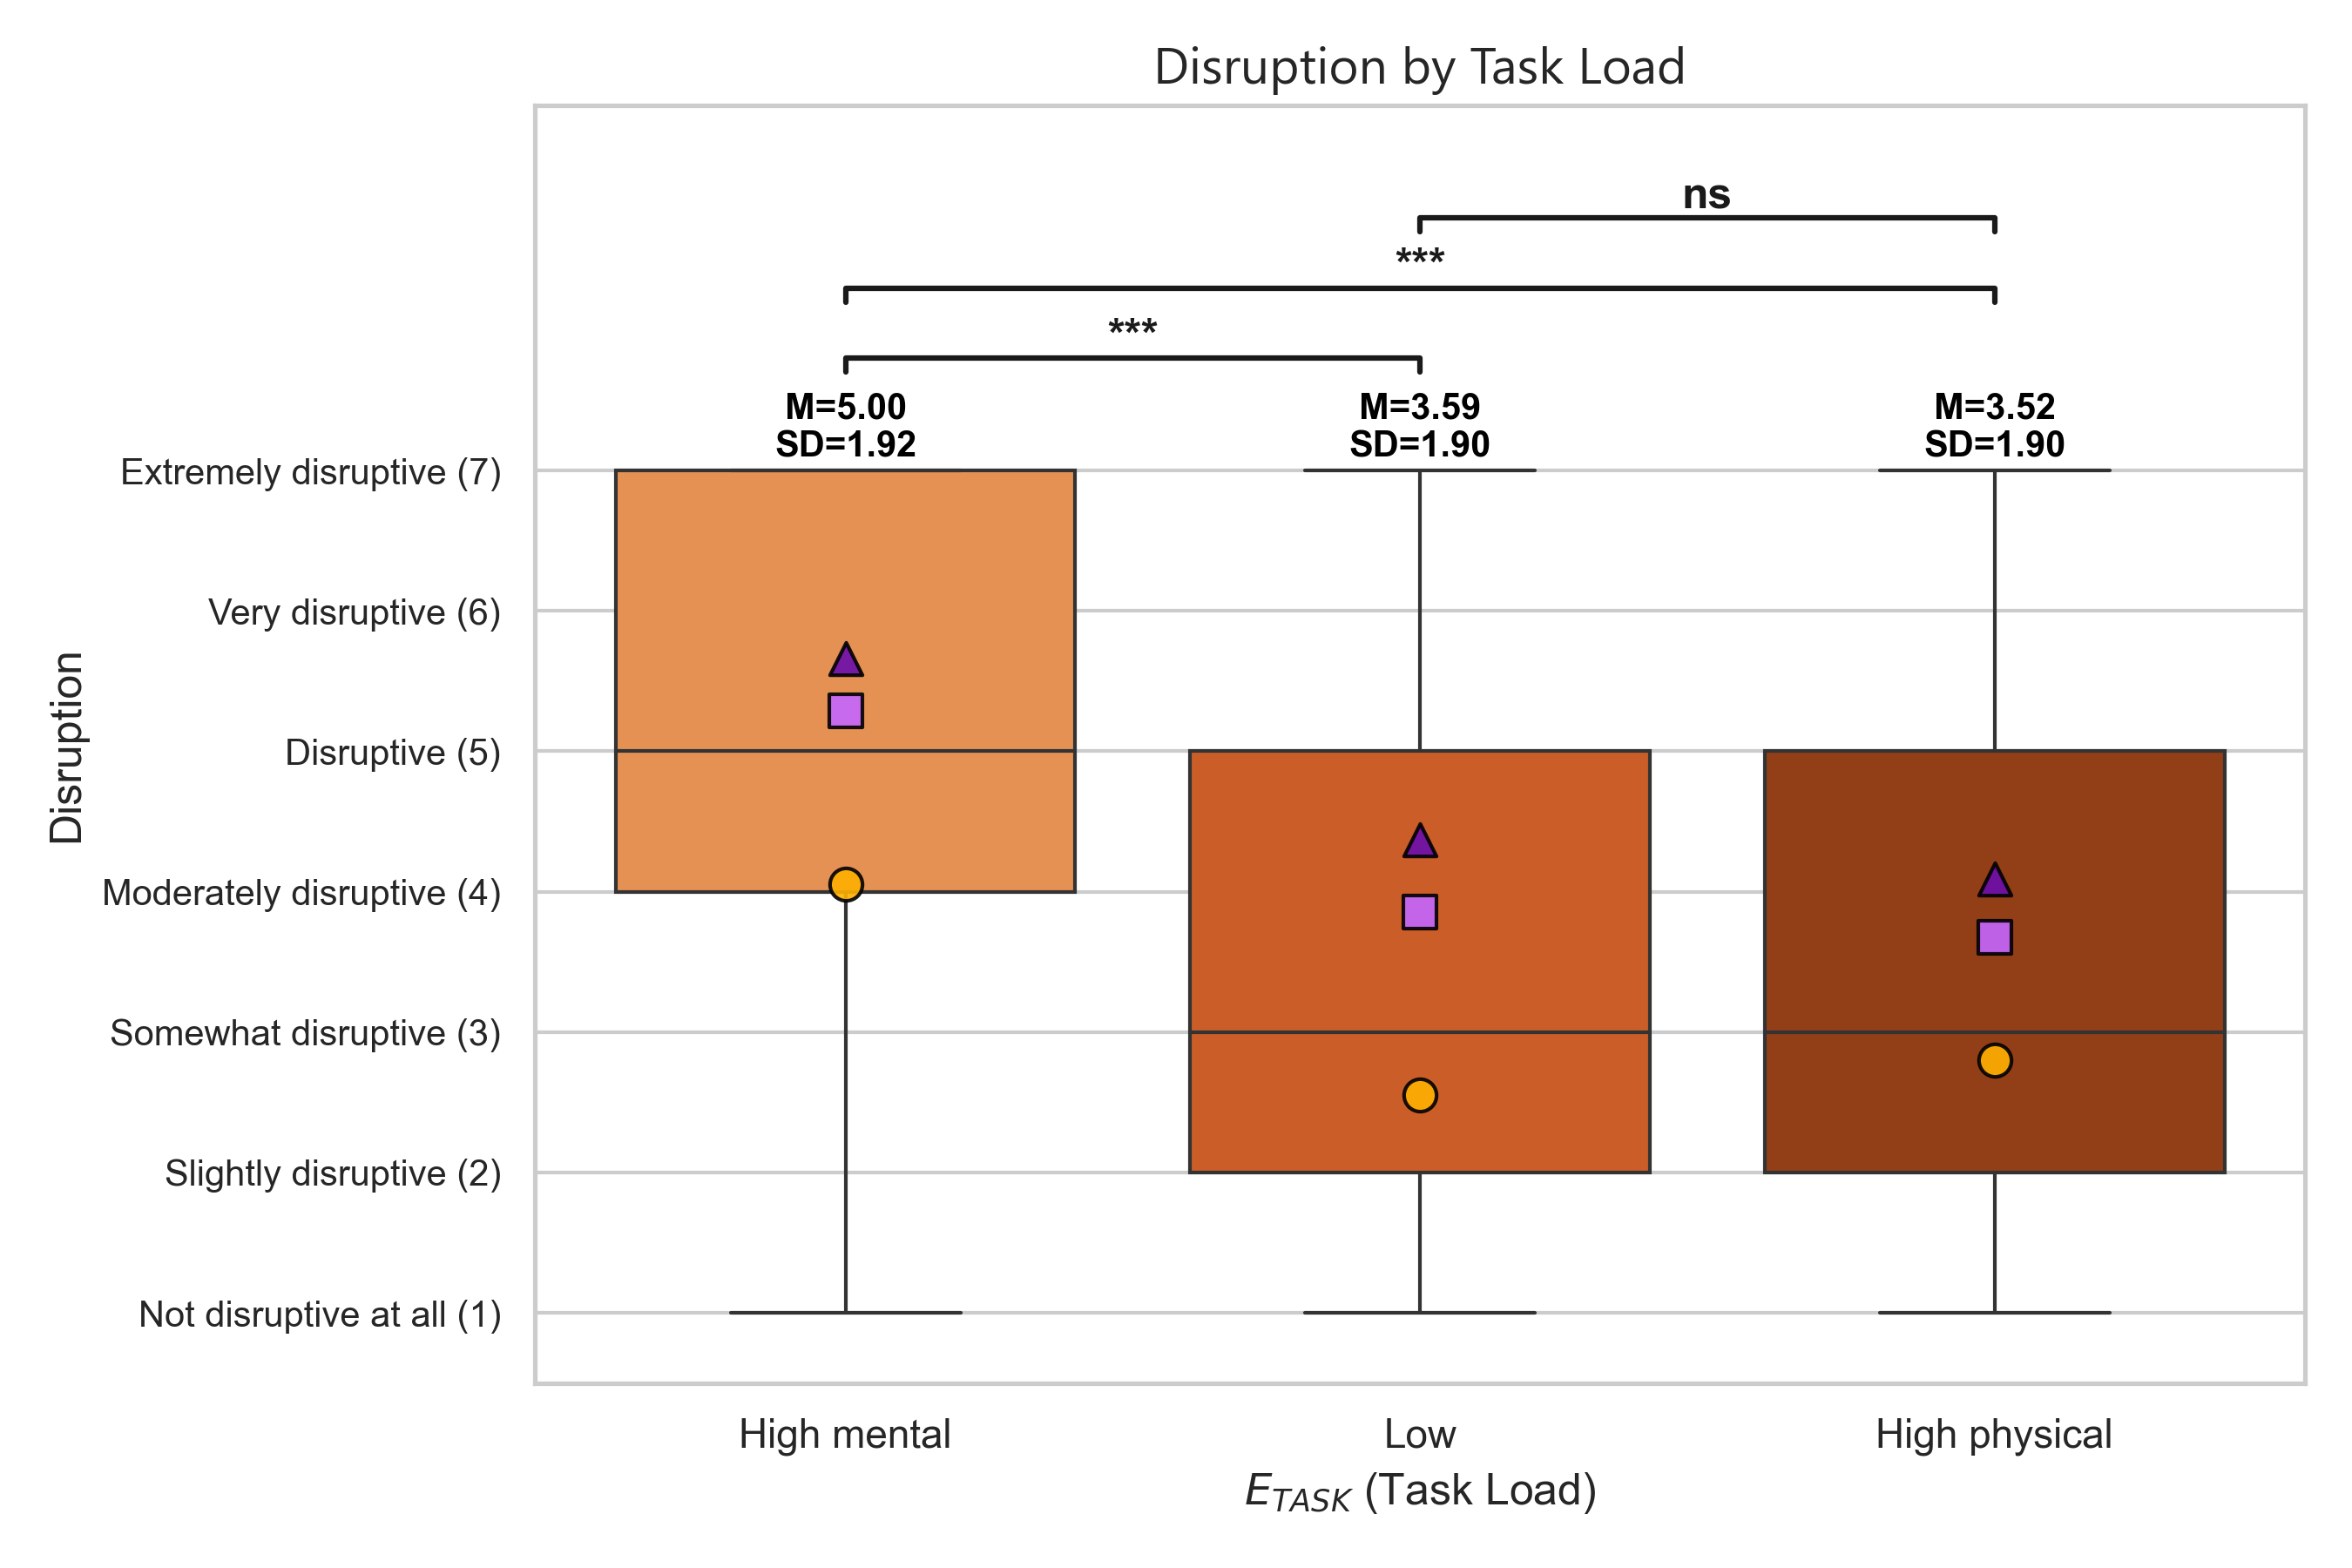
\includegraphics[width=\textwidth]{plots/PrimaryAdvanced_Overall_e_Task_vs_Disruption_inline.png}
        \caption{Overall by Task Load}
    \end{subfigure}
    \hfill
    \begin{subfigure}[b]{0.48\textwidth}
        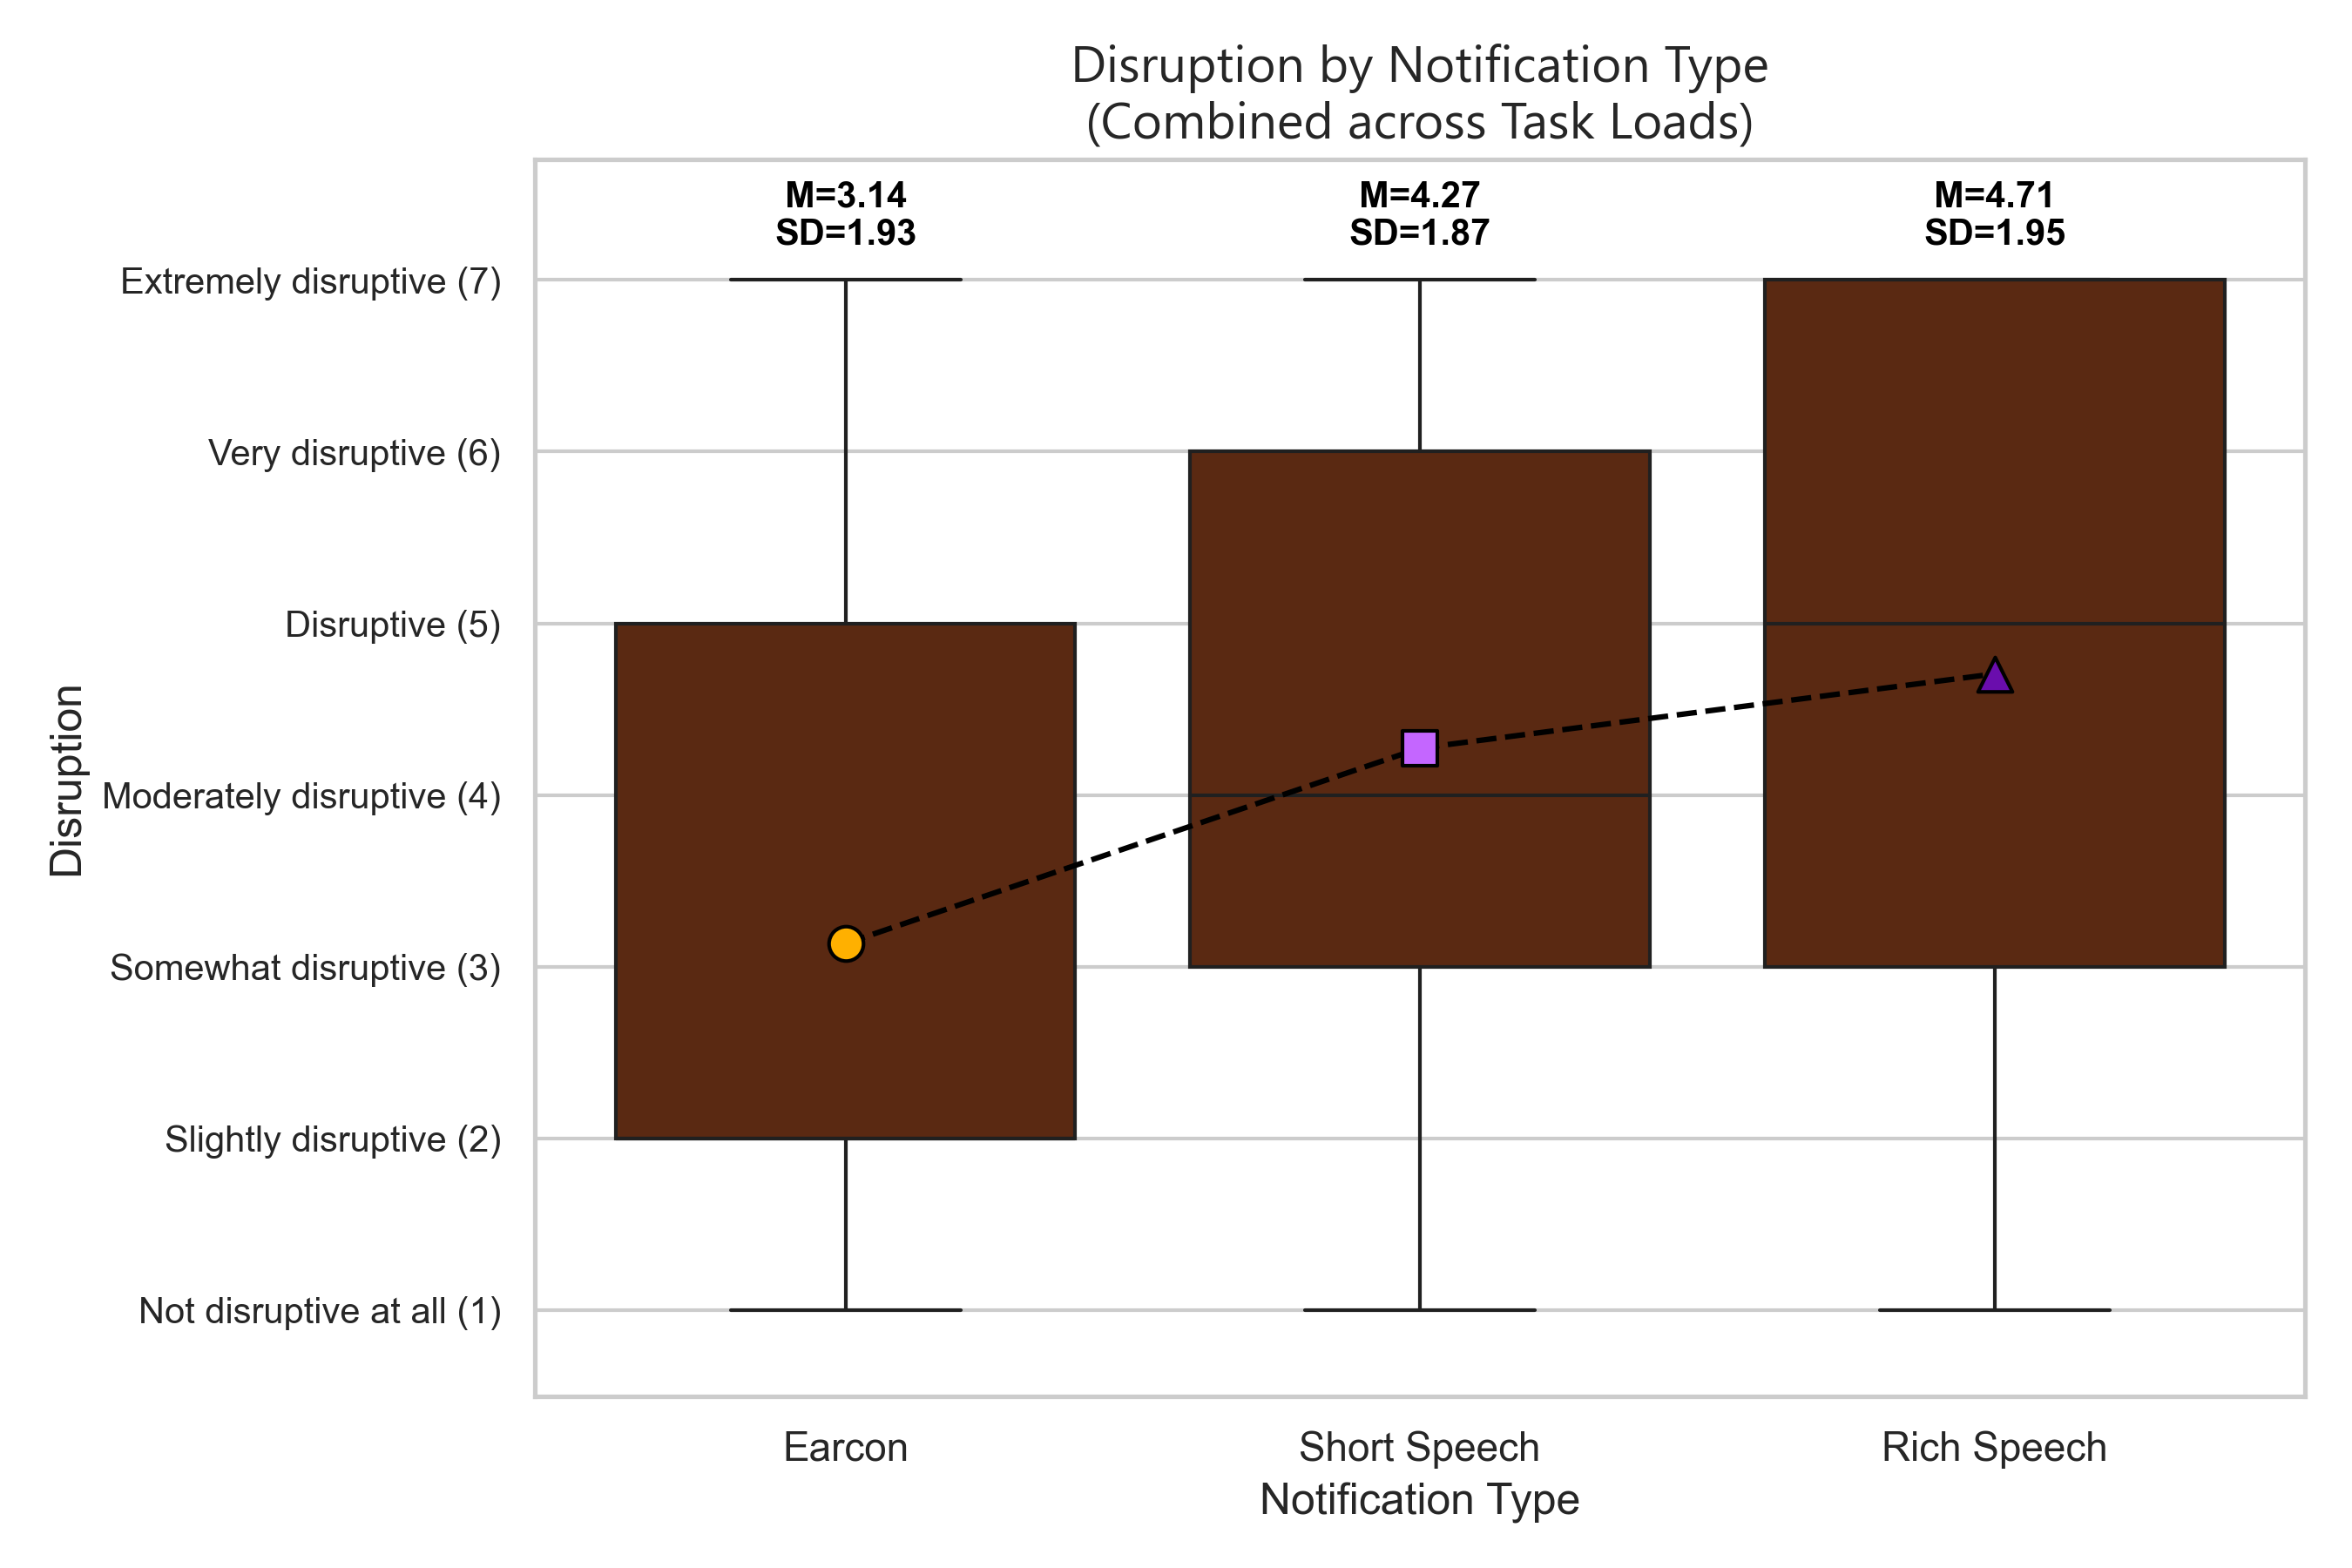
\includegraphics[width=\textwidth]{plots2/Disruption_Combined.png}
        \caption{Overall by Notification Type}
    \end{subfigure}
    
    \vskip\baselineskip % Abstand zwischen oberer und unterer Reihe
    
    % Untere Reihe: Breakdowns per Task Load
    \begin{subfigure}[b]{0.32\textwidth}
        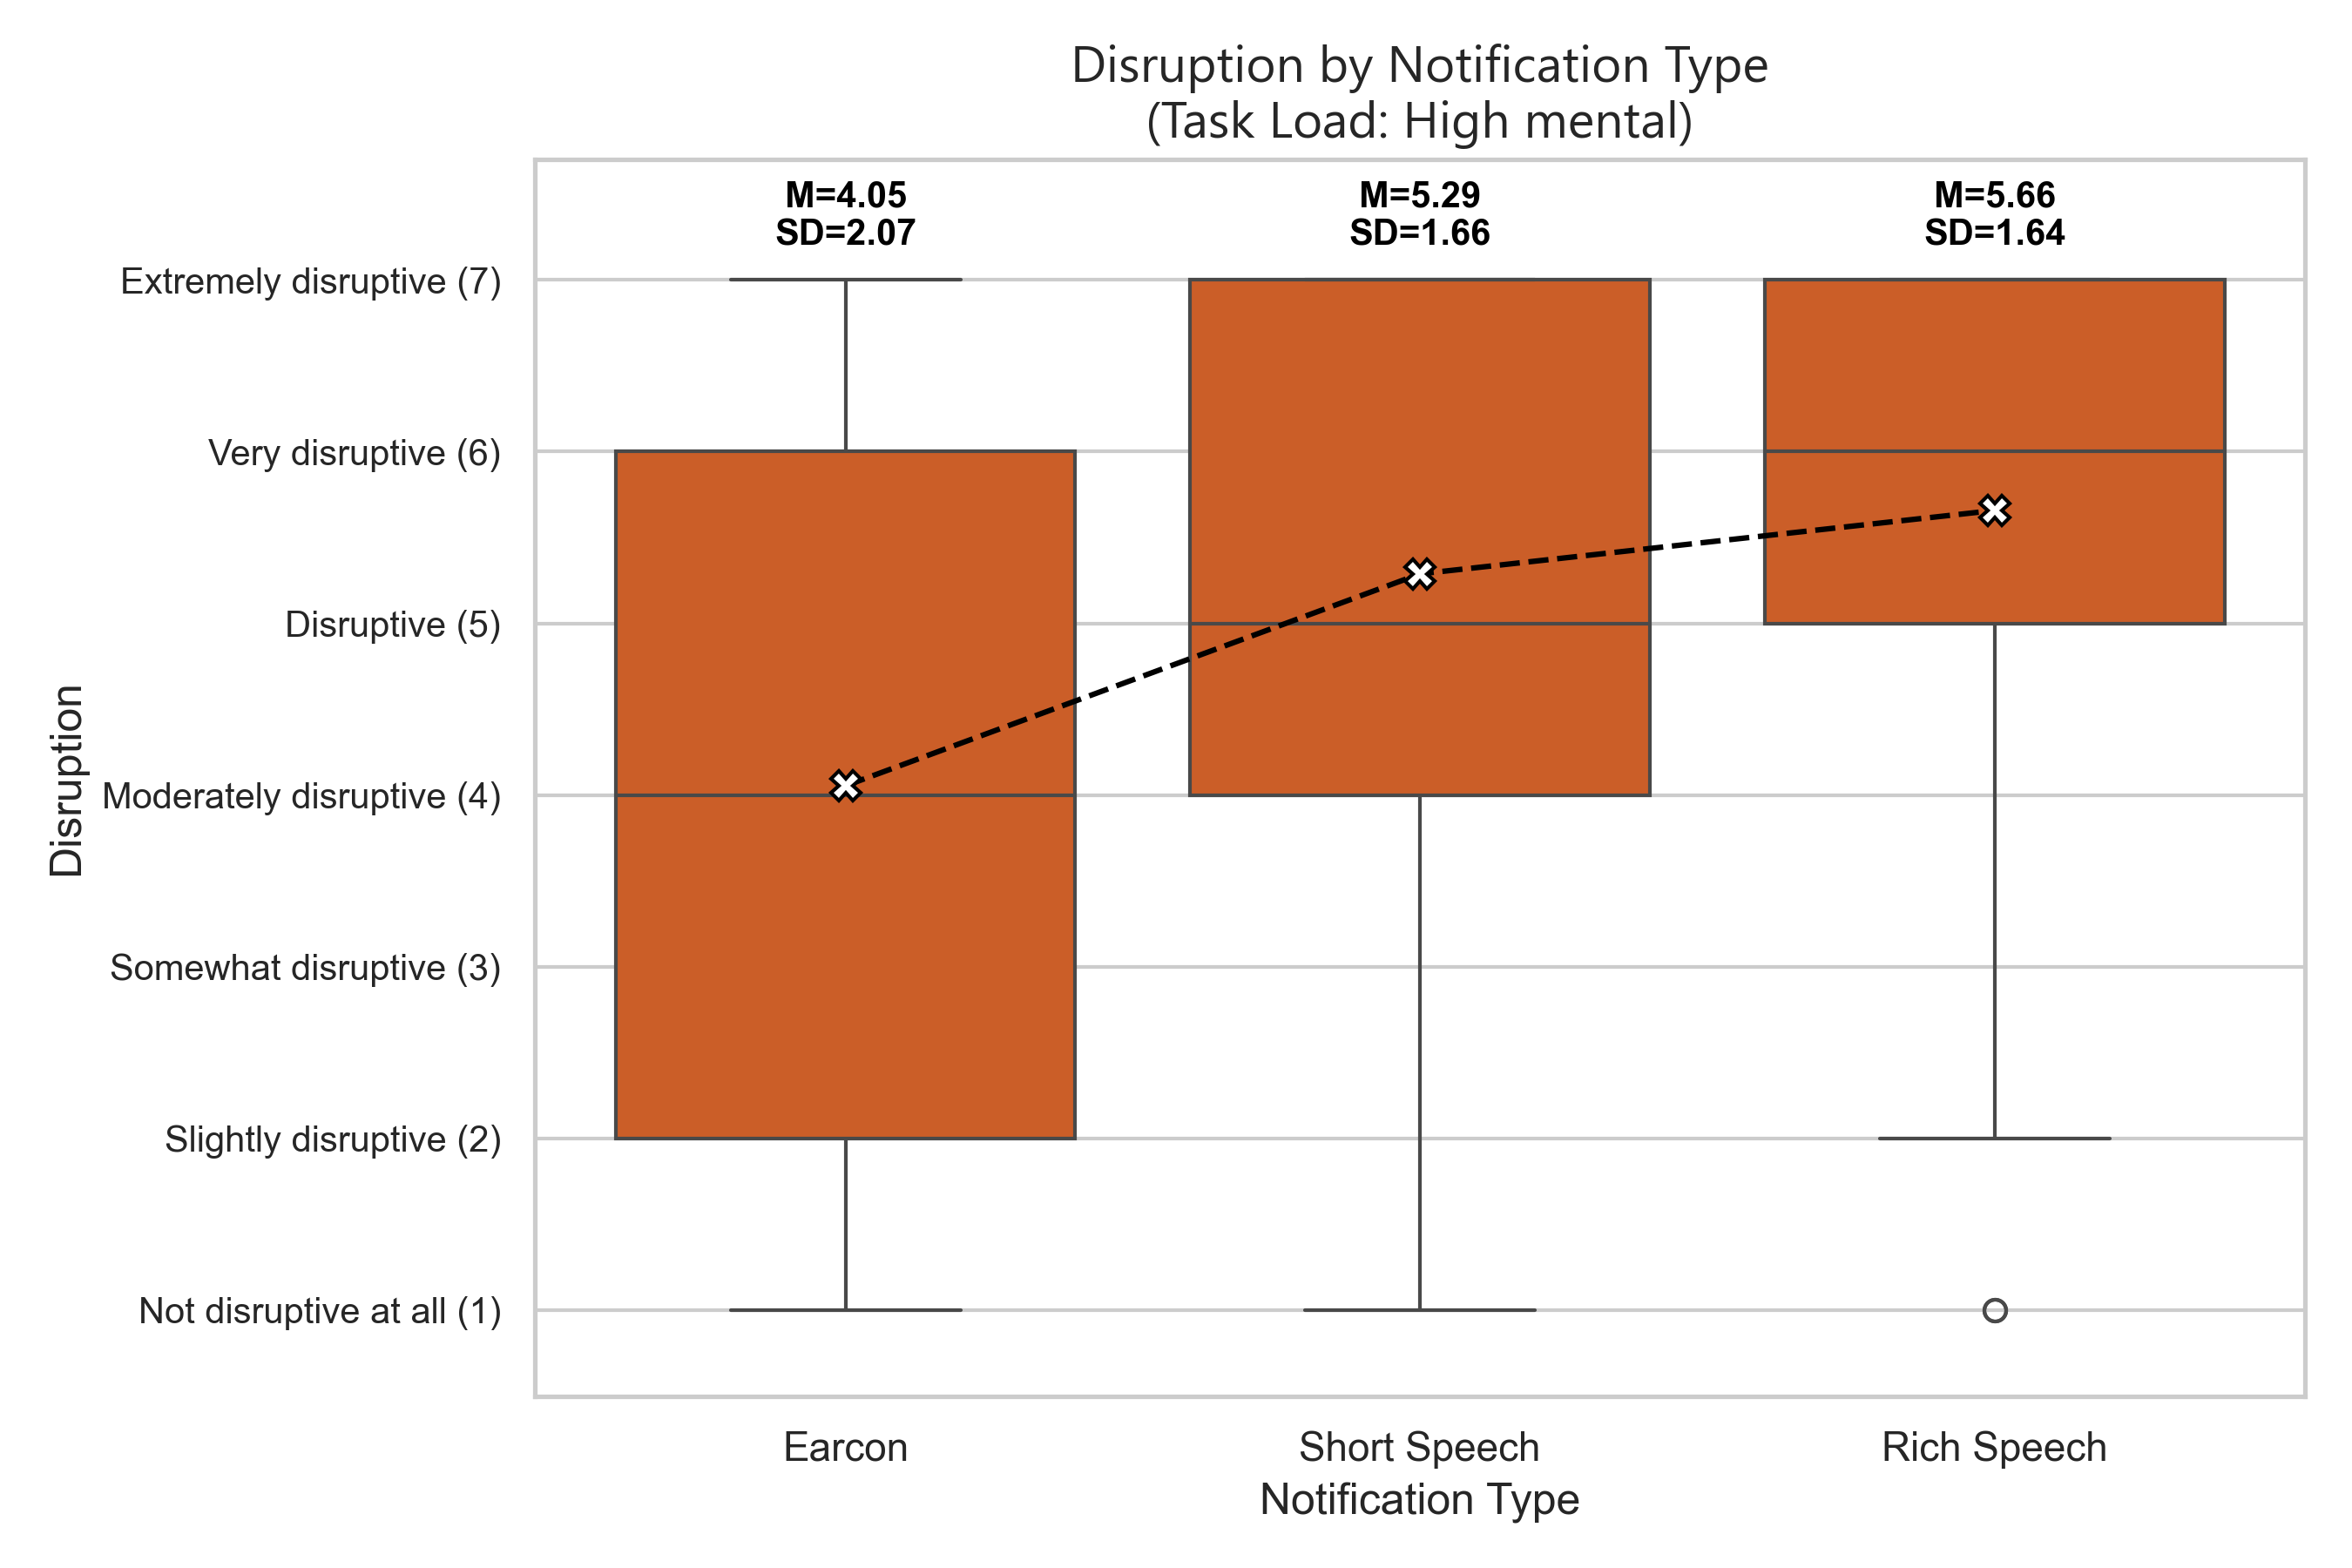
\includegraphics[width=\textwidth]{plots2/Disruption_Highmental.png}
        \caption{High Mental Load}
    \end{subfigure}
    \hfill
    \begin{subfigure}[b]{0.32\textwidth}
        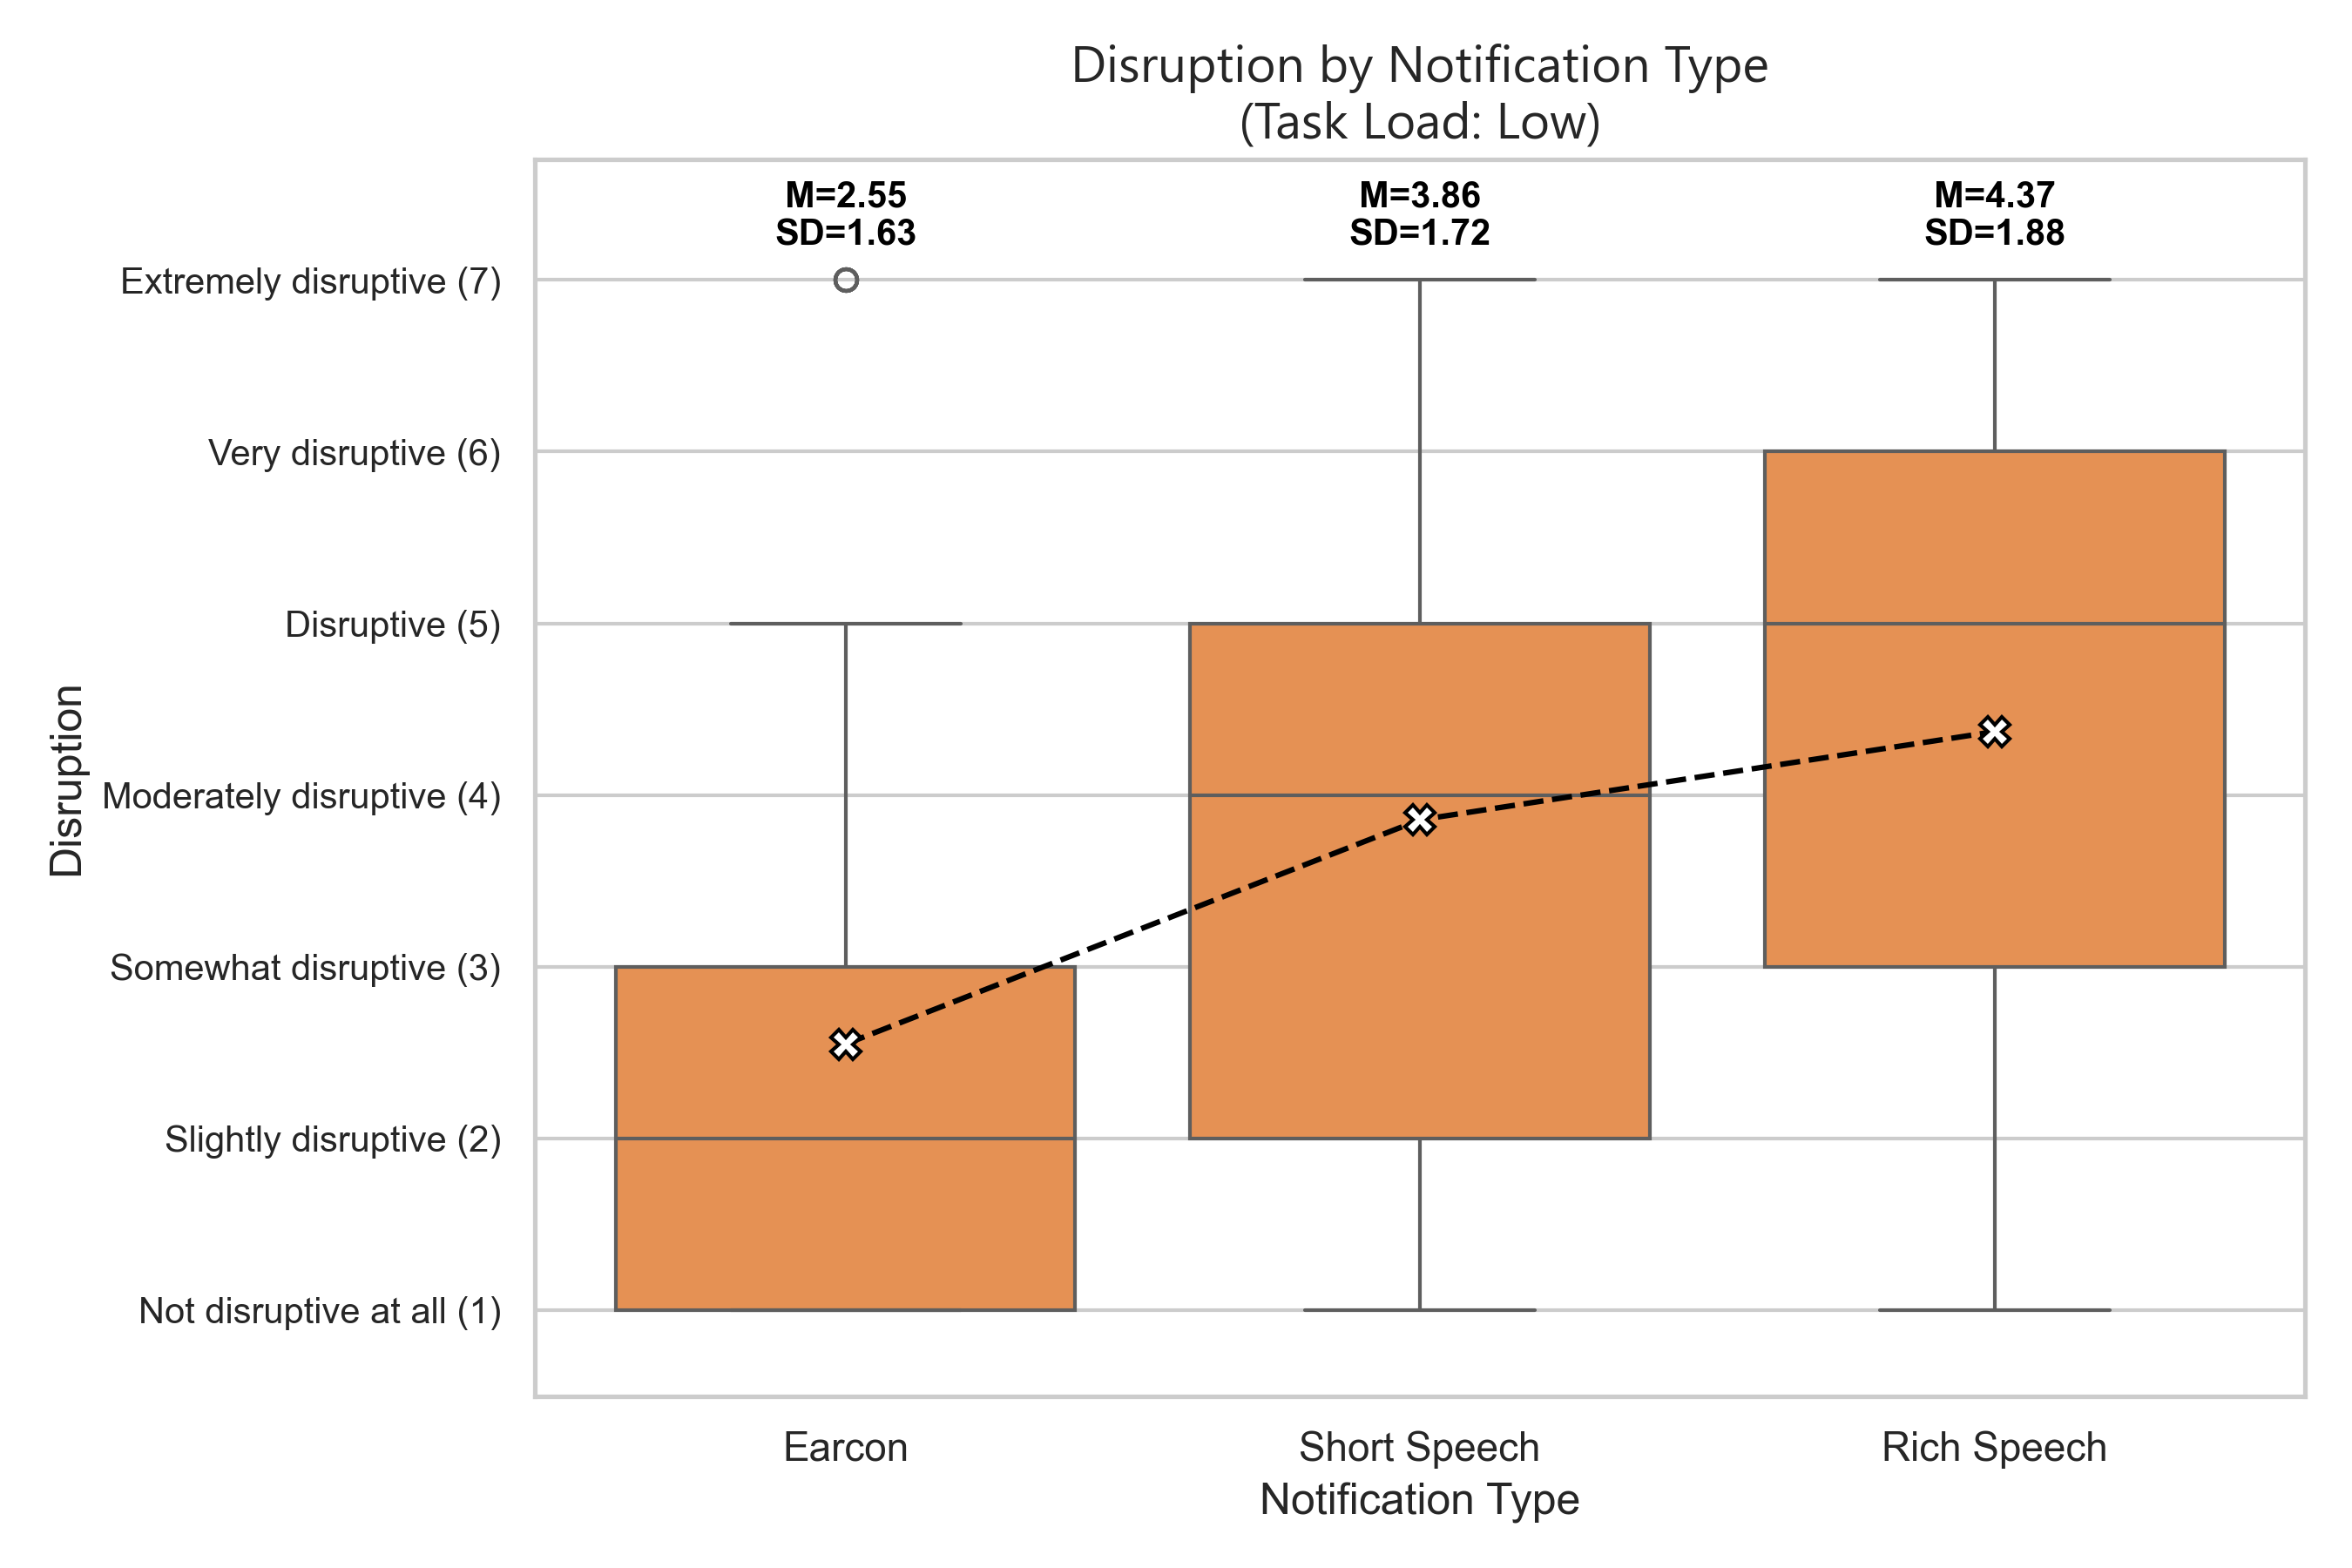
\includegraphics[width=\textwidth]{plots2/Disruption_Low.png}
        \caption{Low Load}
    \end{subfigure}
    \hfill
    \begin{subfigure}[b]{0.32\textwidth}
        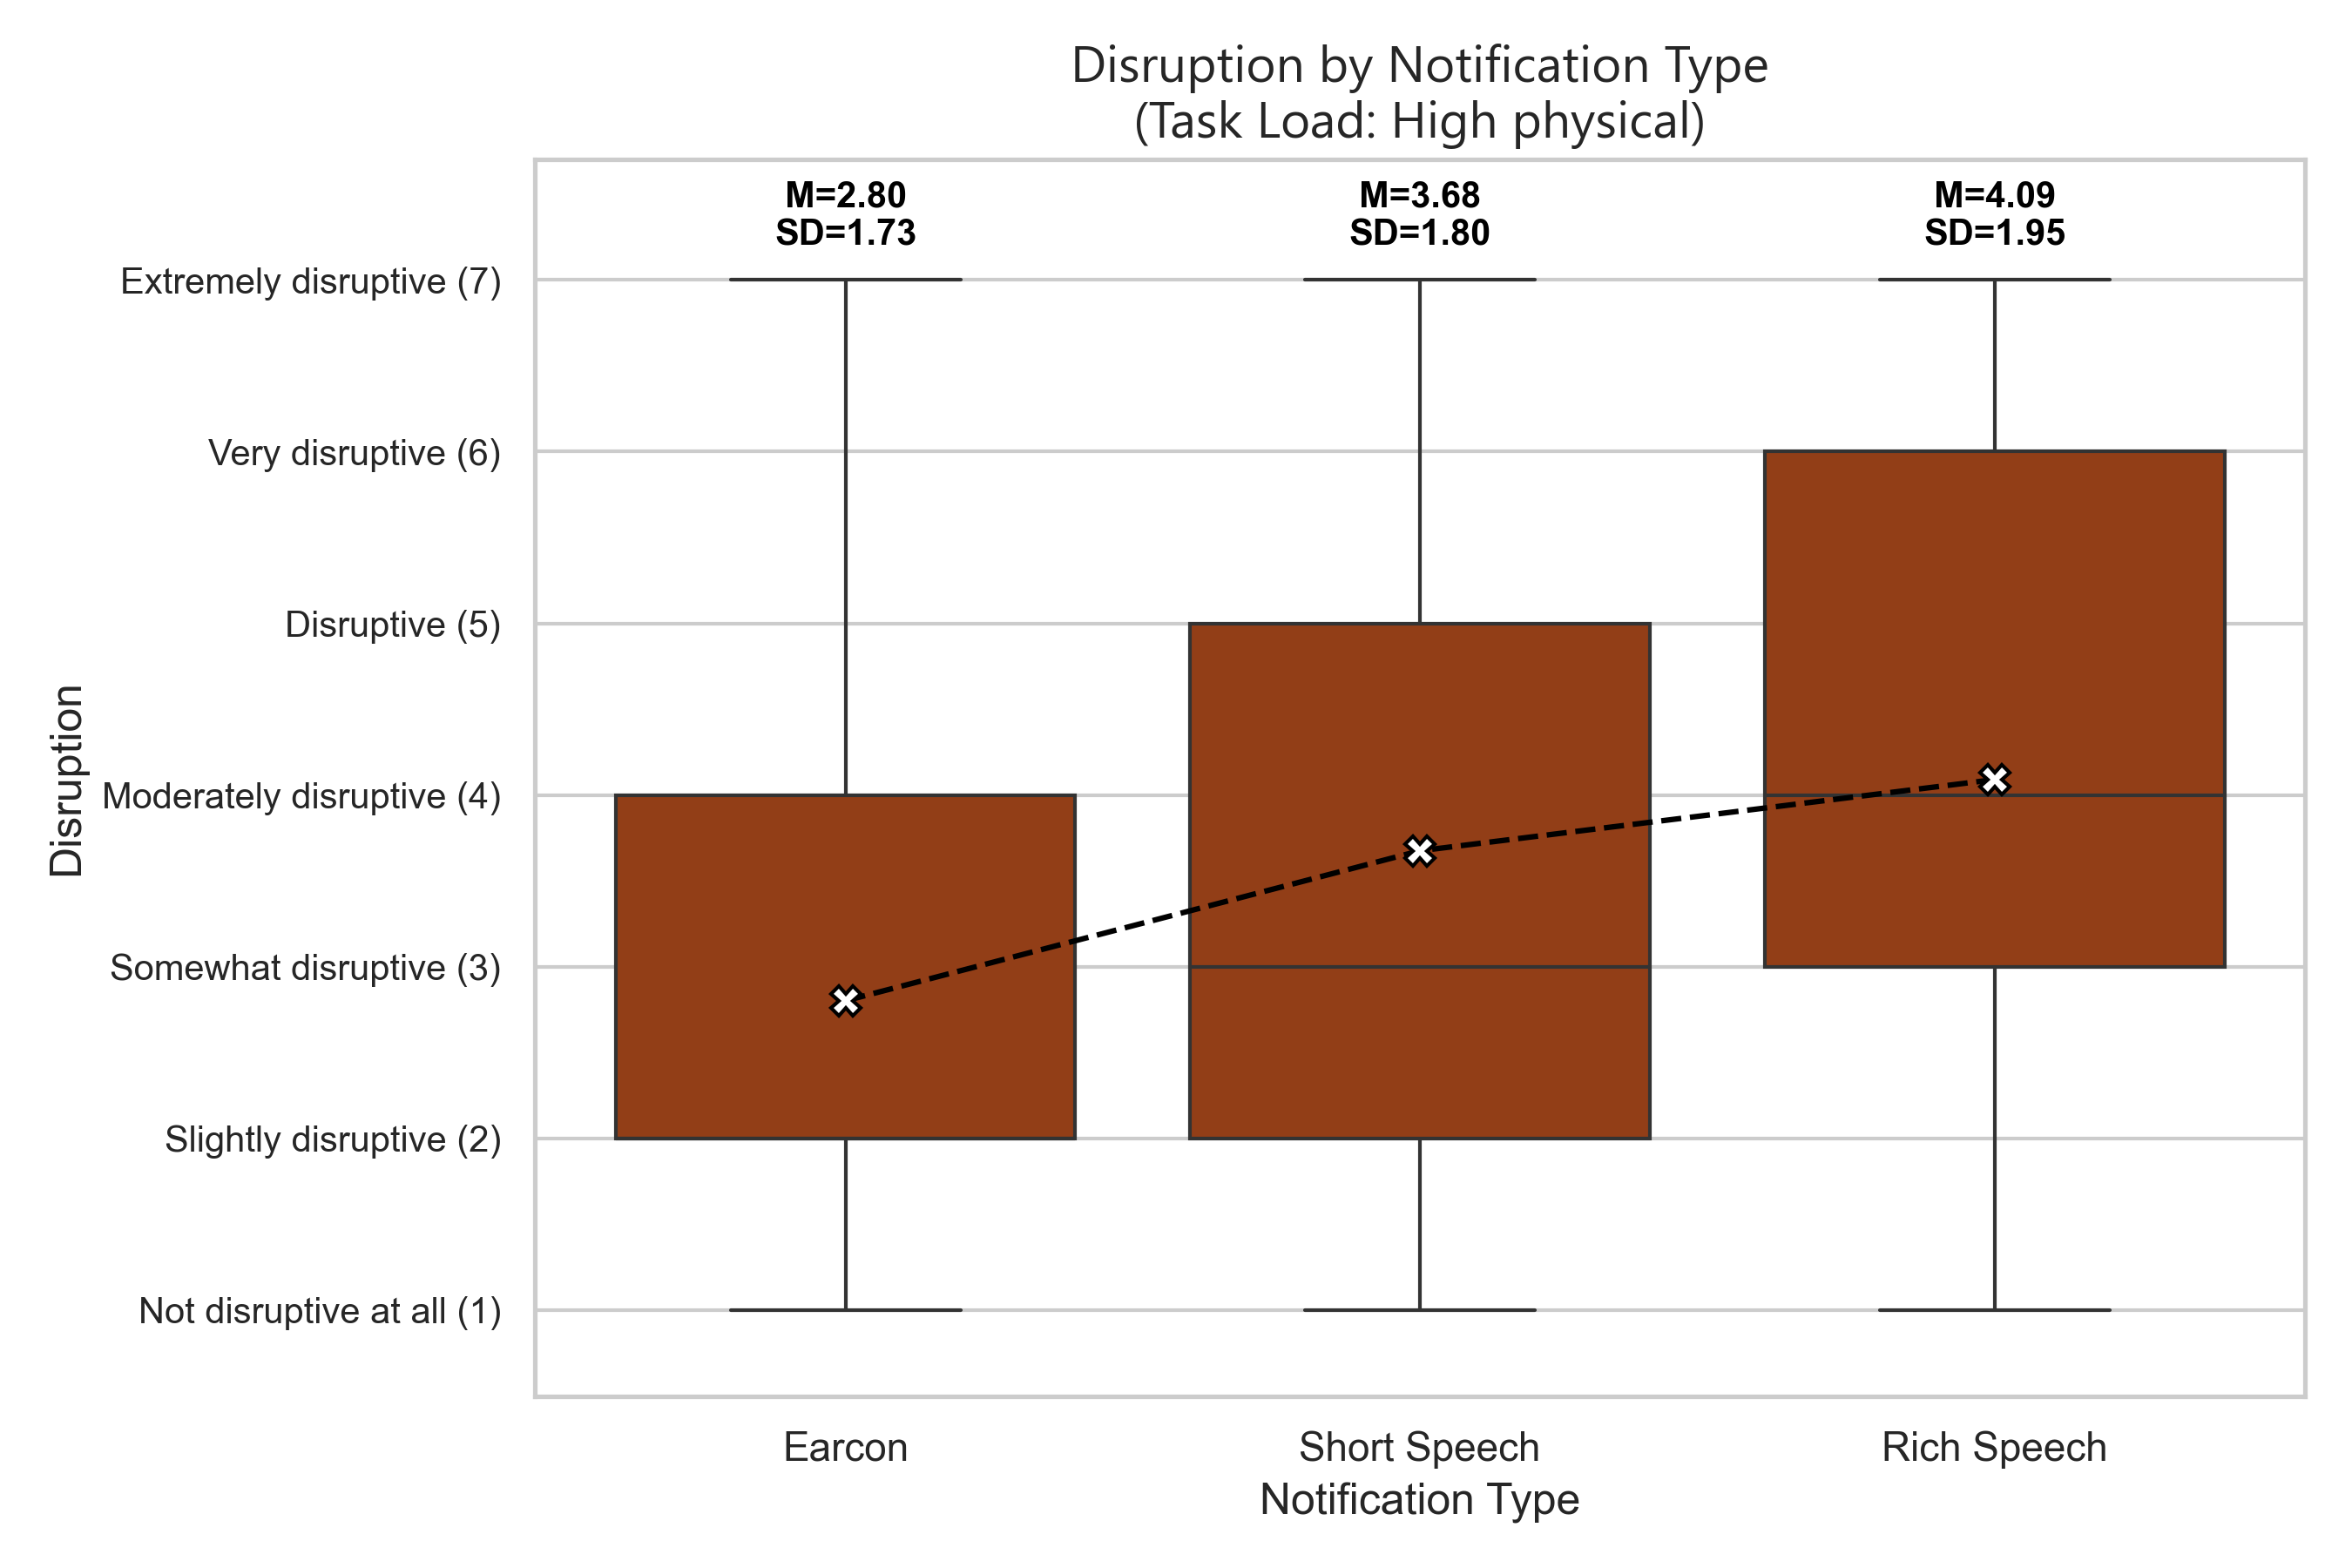
\includegraphics[width=\textwidth]{plots2/Disruption_Highphysical.png}
        \caption{High Physical Load}
    \end{subfigure}
    \caption{Perceived disruption. Plots (a) and (b) visualize the overarching main effects of task load and notification type, corresponding directly to the marginal means derived from the Linear Mixed Model. Plots (c), (d), and (e) break down the disruption caused by each notification type across the three specific task loads.}
    \label{fig:box_disruption}
\end{figure}








\subsection{What Drives Social Acceptability?}
\label{sec:res_social}
To evaluate the impact of context on social norms, we fitted the following model:
$$ \text{Social Acceptability} \sim \text{Notification Type} + \text{Social Setting} + \text{Task Load} + \text{Soundscape} + (1 | \text{Participant}) $$

Social setting heavily dictated whether an auditory notification was deemed acceptable. When transitioning from being alone ($M = 5.58$) to an interactive setting ($M = 4.04$), social acceptability dropped drastically ($\Delta M = -1.54, p < .001$), as seen in \autoref{fig:box_social}a. Crucially, transitioning from the interactive to the passive setting produced a significant increase in social acceptability ($\Delta M = 1.32, p < .001$), confirming that the social penalty is specifically tied to active interpersonal engagement. While a passive social setting also trended slightly negatively compared to being alone ($M = 5.35$; $\Delta M = -0.22, p = .048$), this effect did not survive the strict Bonferroni correction and is thus considered not statistically significant in our rigorous model.

Regarding notification types, speech-based formats were heavily penalized in social contexts. Both Short Speech ($\Delta M = -0.63, p < .001$) and Rich Speech ($\Delta M = -0.86, p < .001$) were viewed as significantly less socially acceptable than simple Earcons. \autoref{fig:box_social}b illustrates this penalty across all three notification formats.

A closer inspection of the descriptive means highlights how the social context disproportionately affects speech notifications. When users are alone, the drop in acceptability from an Earcon ($M = 5.87$) to Rich Speech ($M = 5.33$) is relatively small, with all types remaining highly acceptable. A similar, moderate decline is visible during passive co-presence (Earcon: $M = 5.77$ vs. Rich Speech: $M = 5.06$). However, during interactive co-presence, while Earcons maintain a neutral-to-positive acceptability ($M = 4.81$), the acceptability of Short Speech ($M = 3.82$) and Rich Speech ($M = 3.49$) falls sharply. This indicates that speech notifications are not universally penalized in public, but rather specifically during active social interactions.

\begin{figure}[H]
    \centering
    % Obere Reihe: Main Effects
    \begin{subfigure}[b]{0.48\textwidth}
        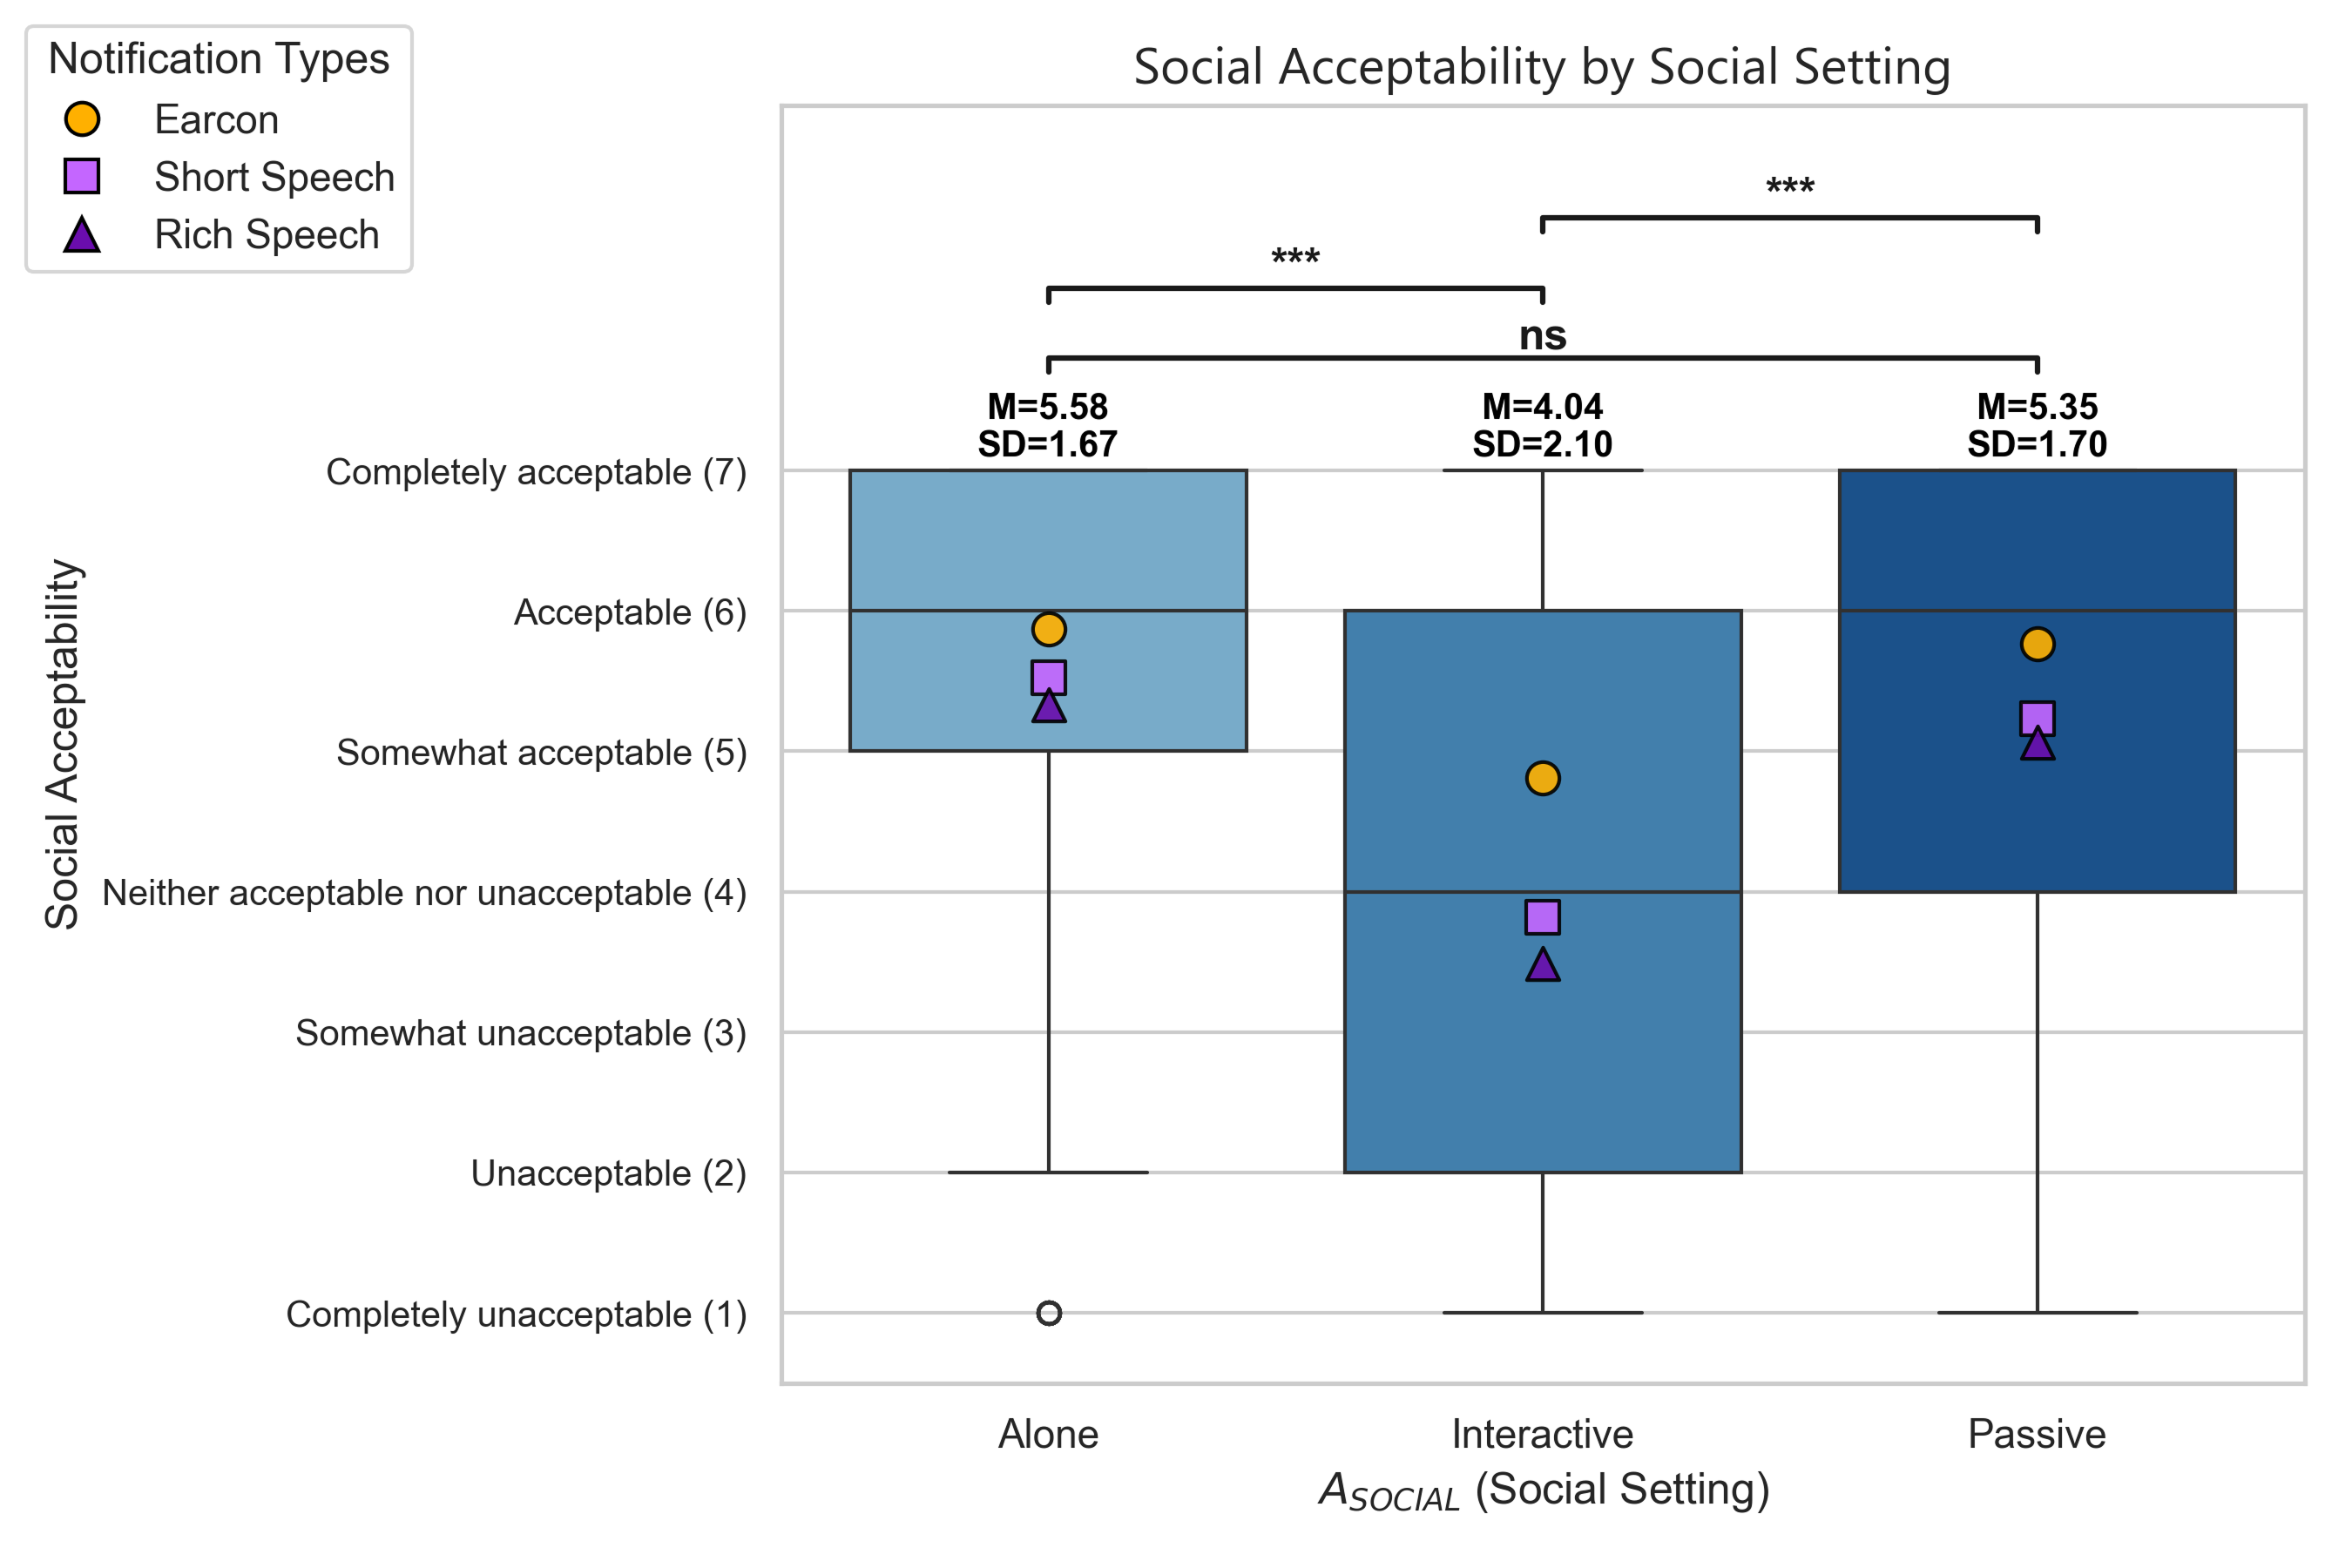
\includegraphics[width=\textwidth]{plots/PrimaryAdvanced_Overall_Asocial_vs_Social_Acceptability_inline.png}
        \caption{Overall by Social Setting}
    \end{subfigure}
    \hfill
    \begin{subfigure}[b]{0.48\textwidth}
        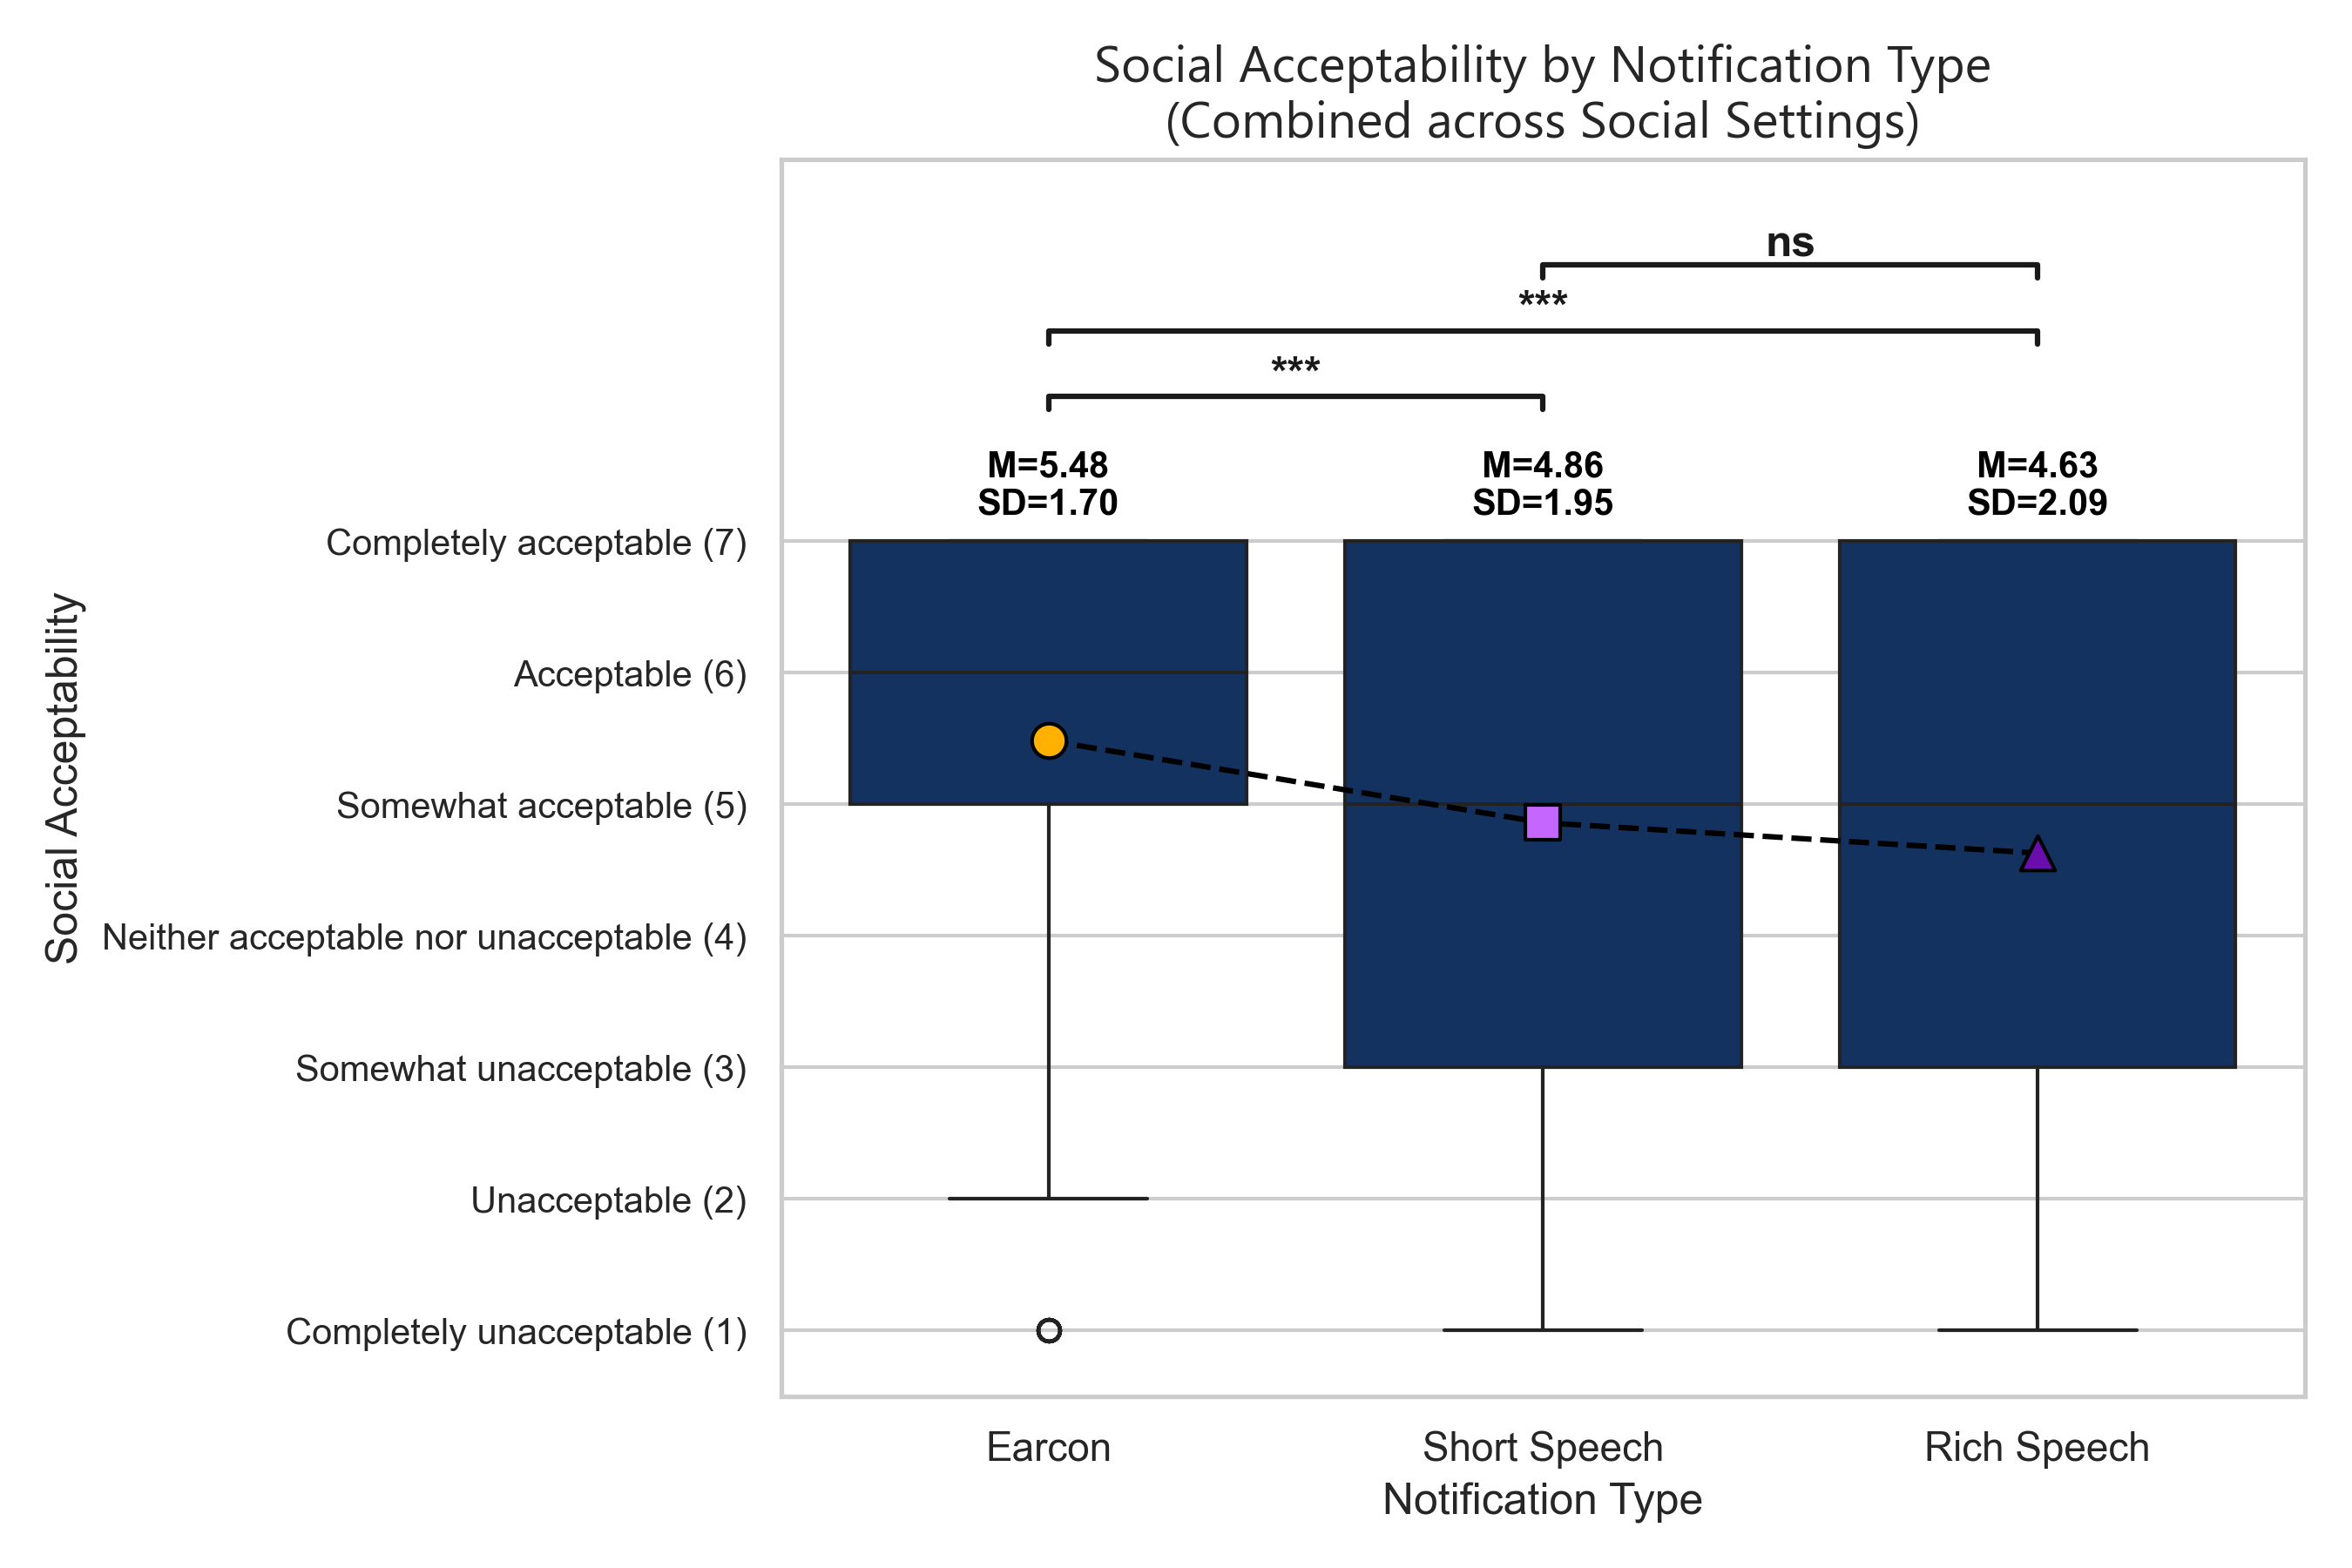
\includegraphics[width=\textwidth]{plots2/SocialAcceptability_Combined.png}
        \caption{Overall by Notification Type}
    \end{subfigure}
    
    \vskip\baselineskip % Abstand zwischen oberer und unterer Reihe
    
    % Untere Reihe: Breakdowns per Social Setting
    \begin{subfigure}[b]{0.32\textwidth}
        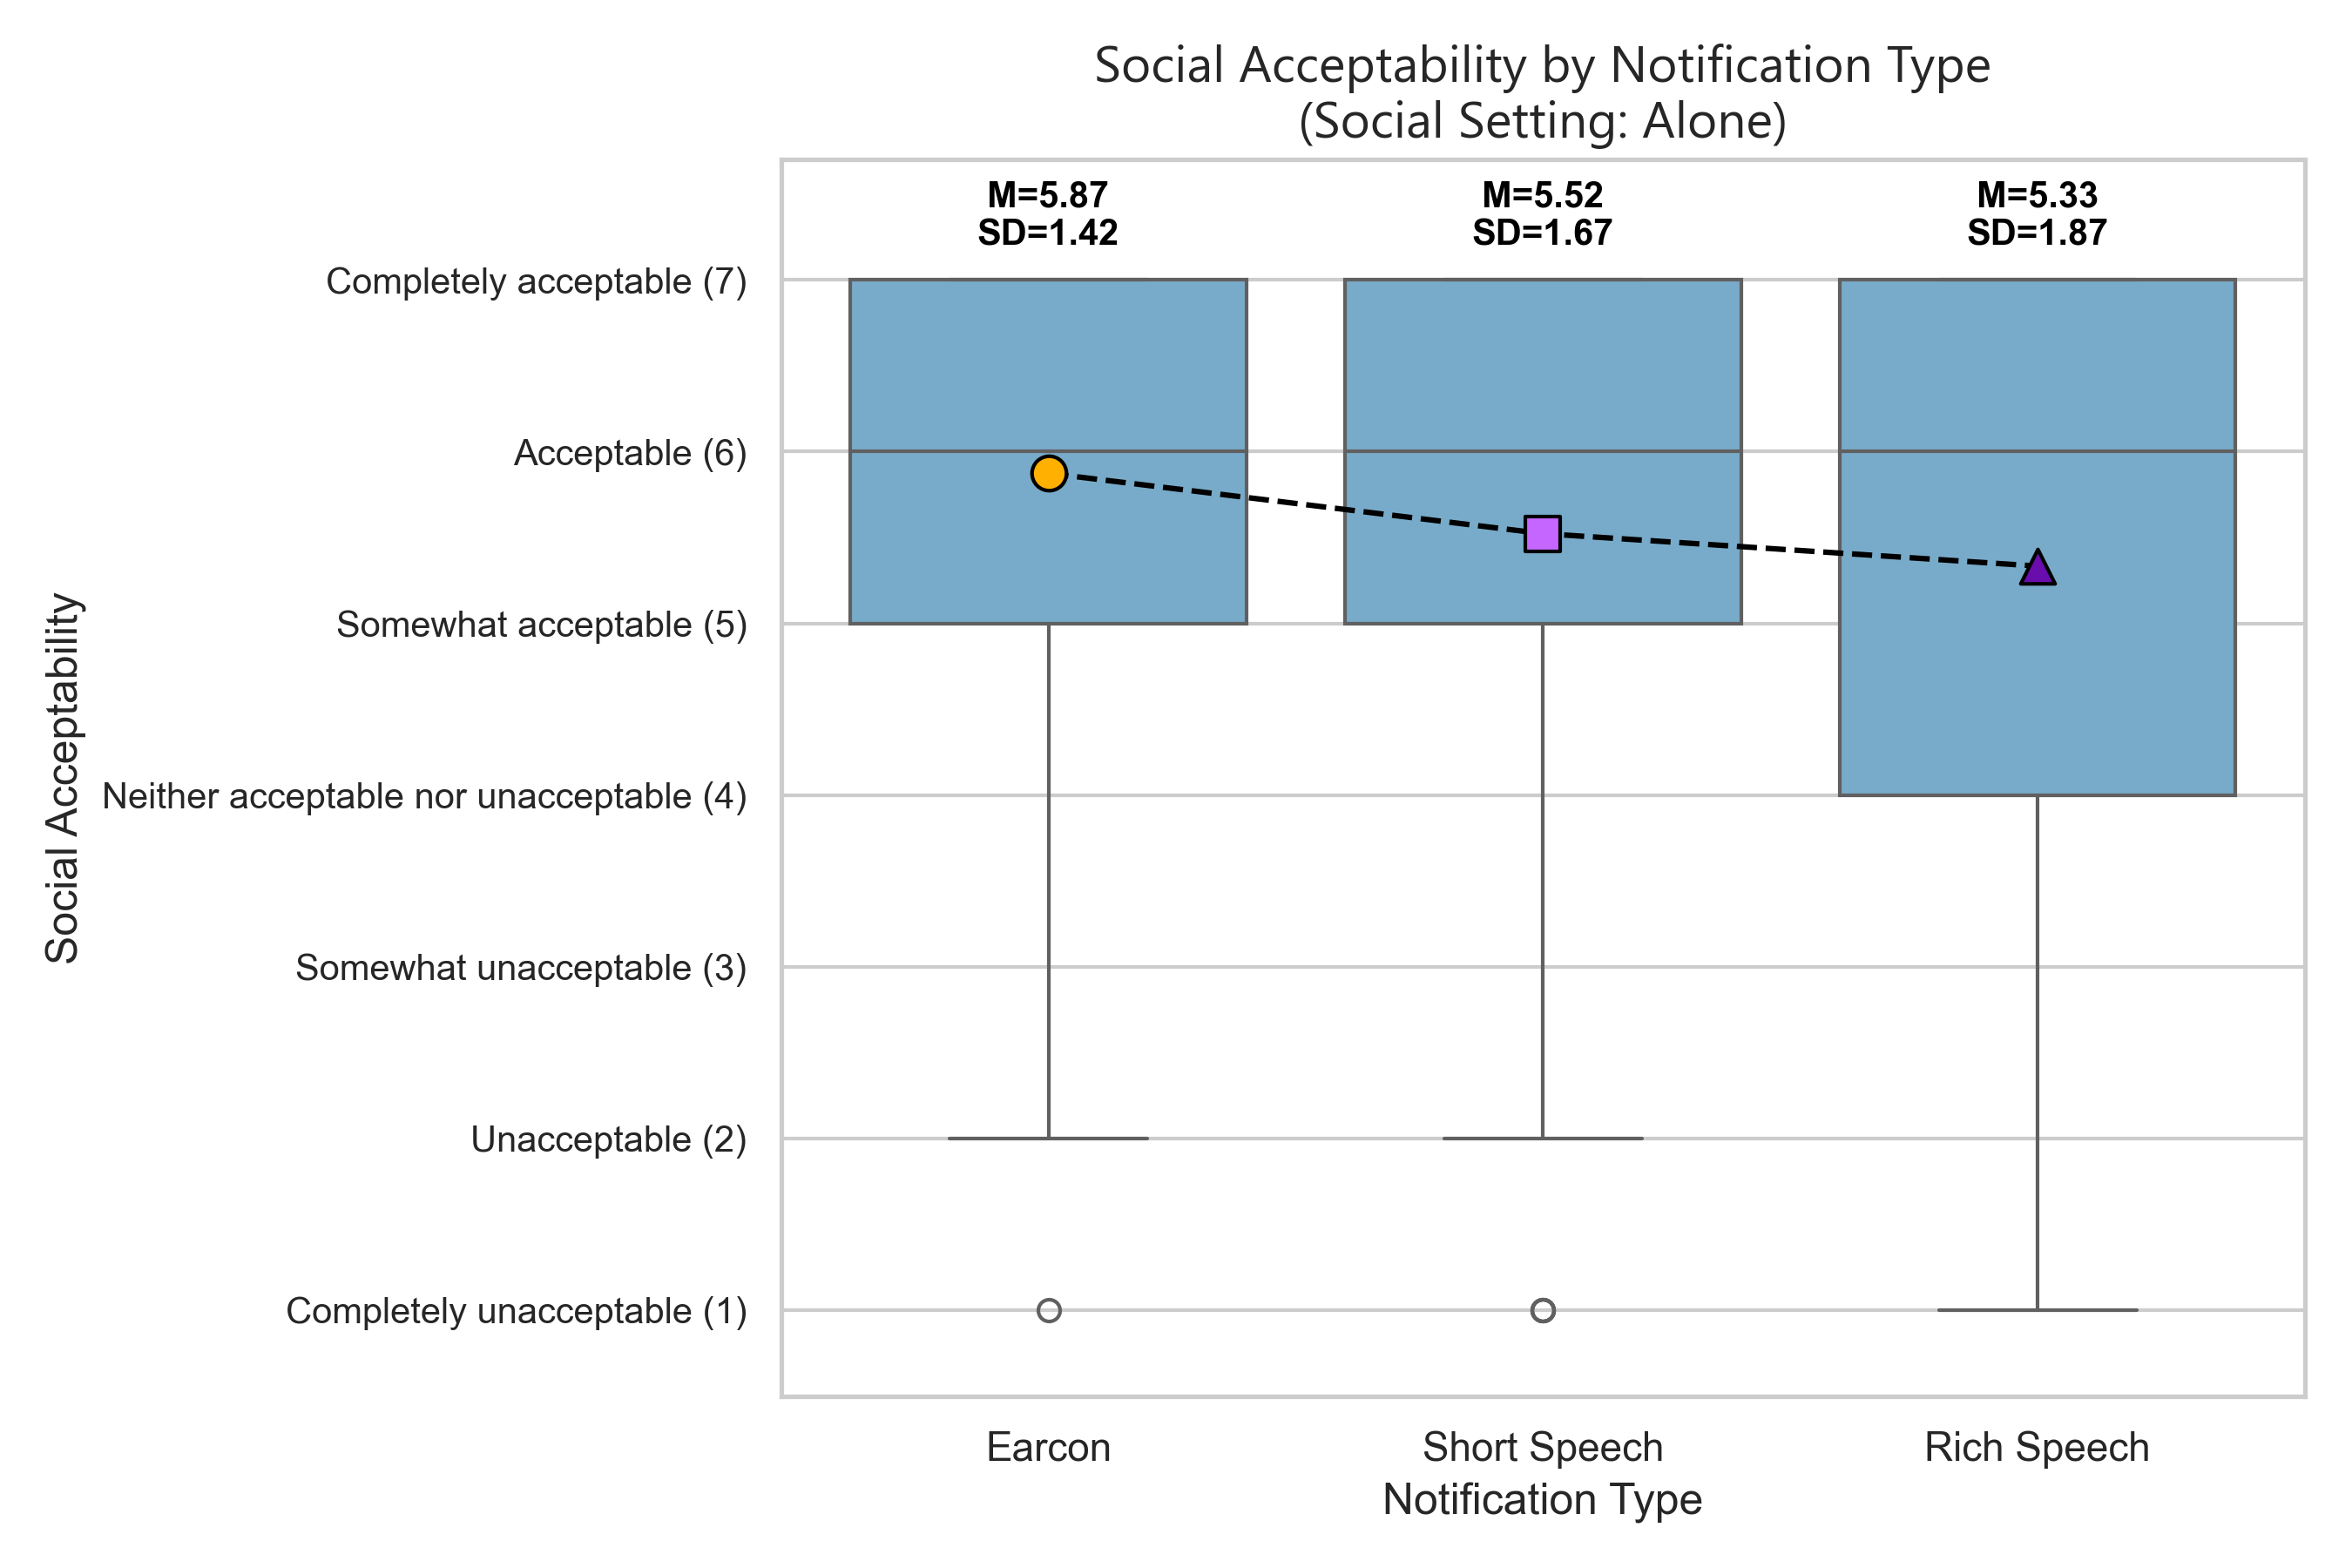
\includegraphics[width=\textwidth]{plots2/SocialAcceptability_Alone.png}
        \caption{Alone}
    \end{subfigure}
    \hfill
    \begin{subfigure}[b]{0.32\textwidth}
        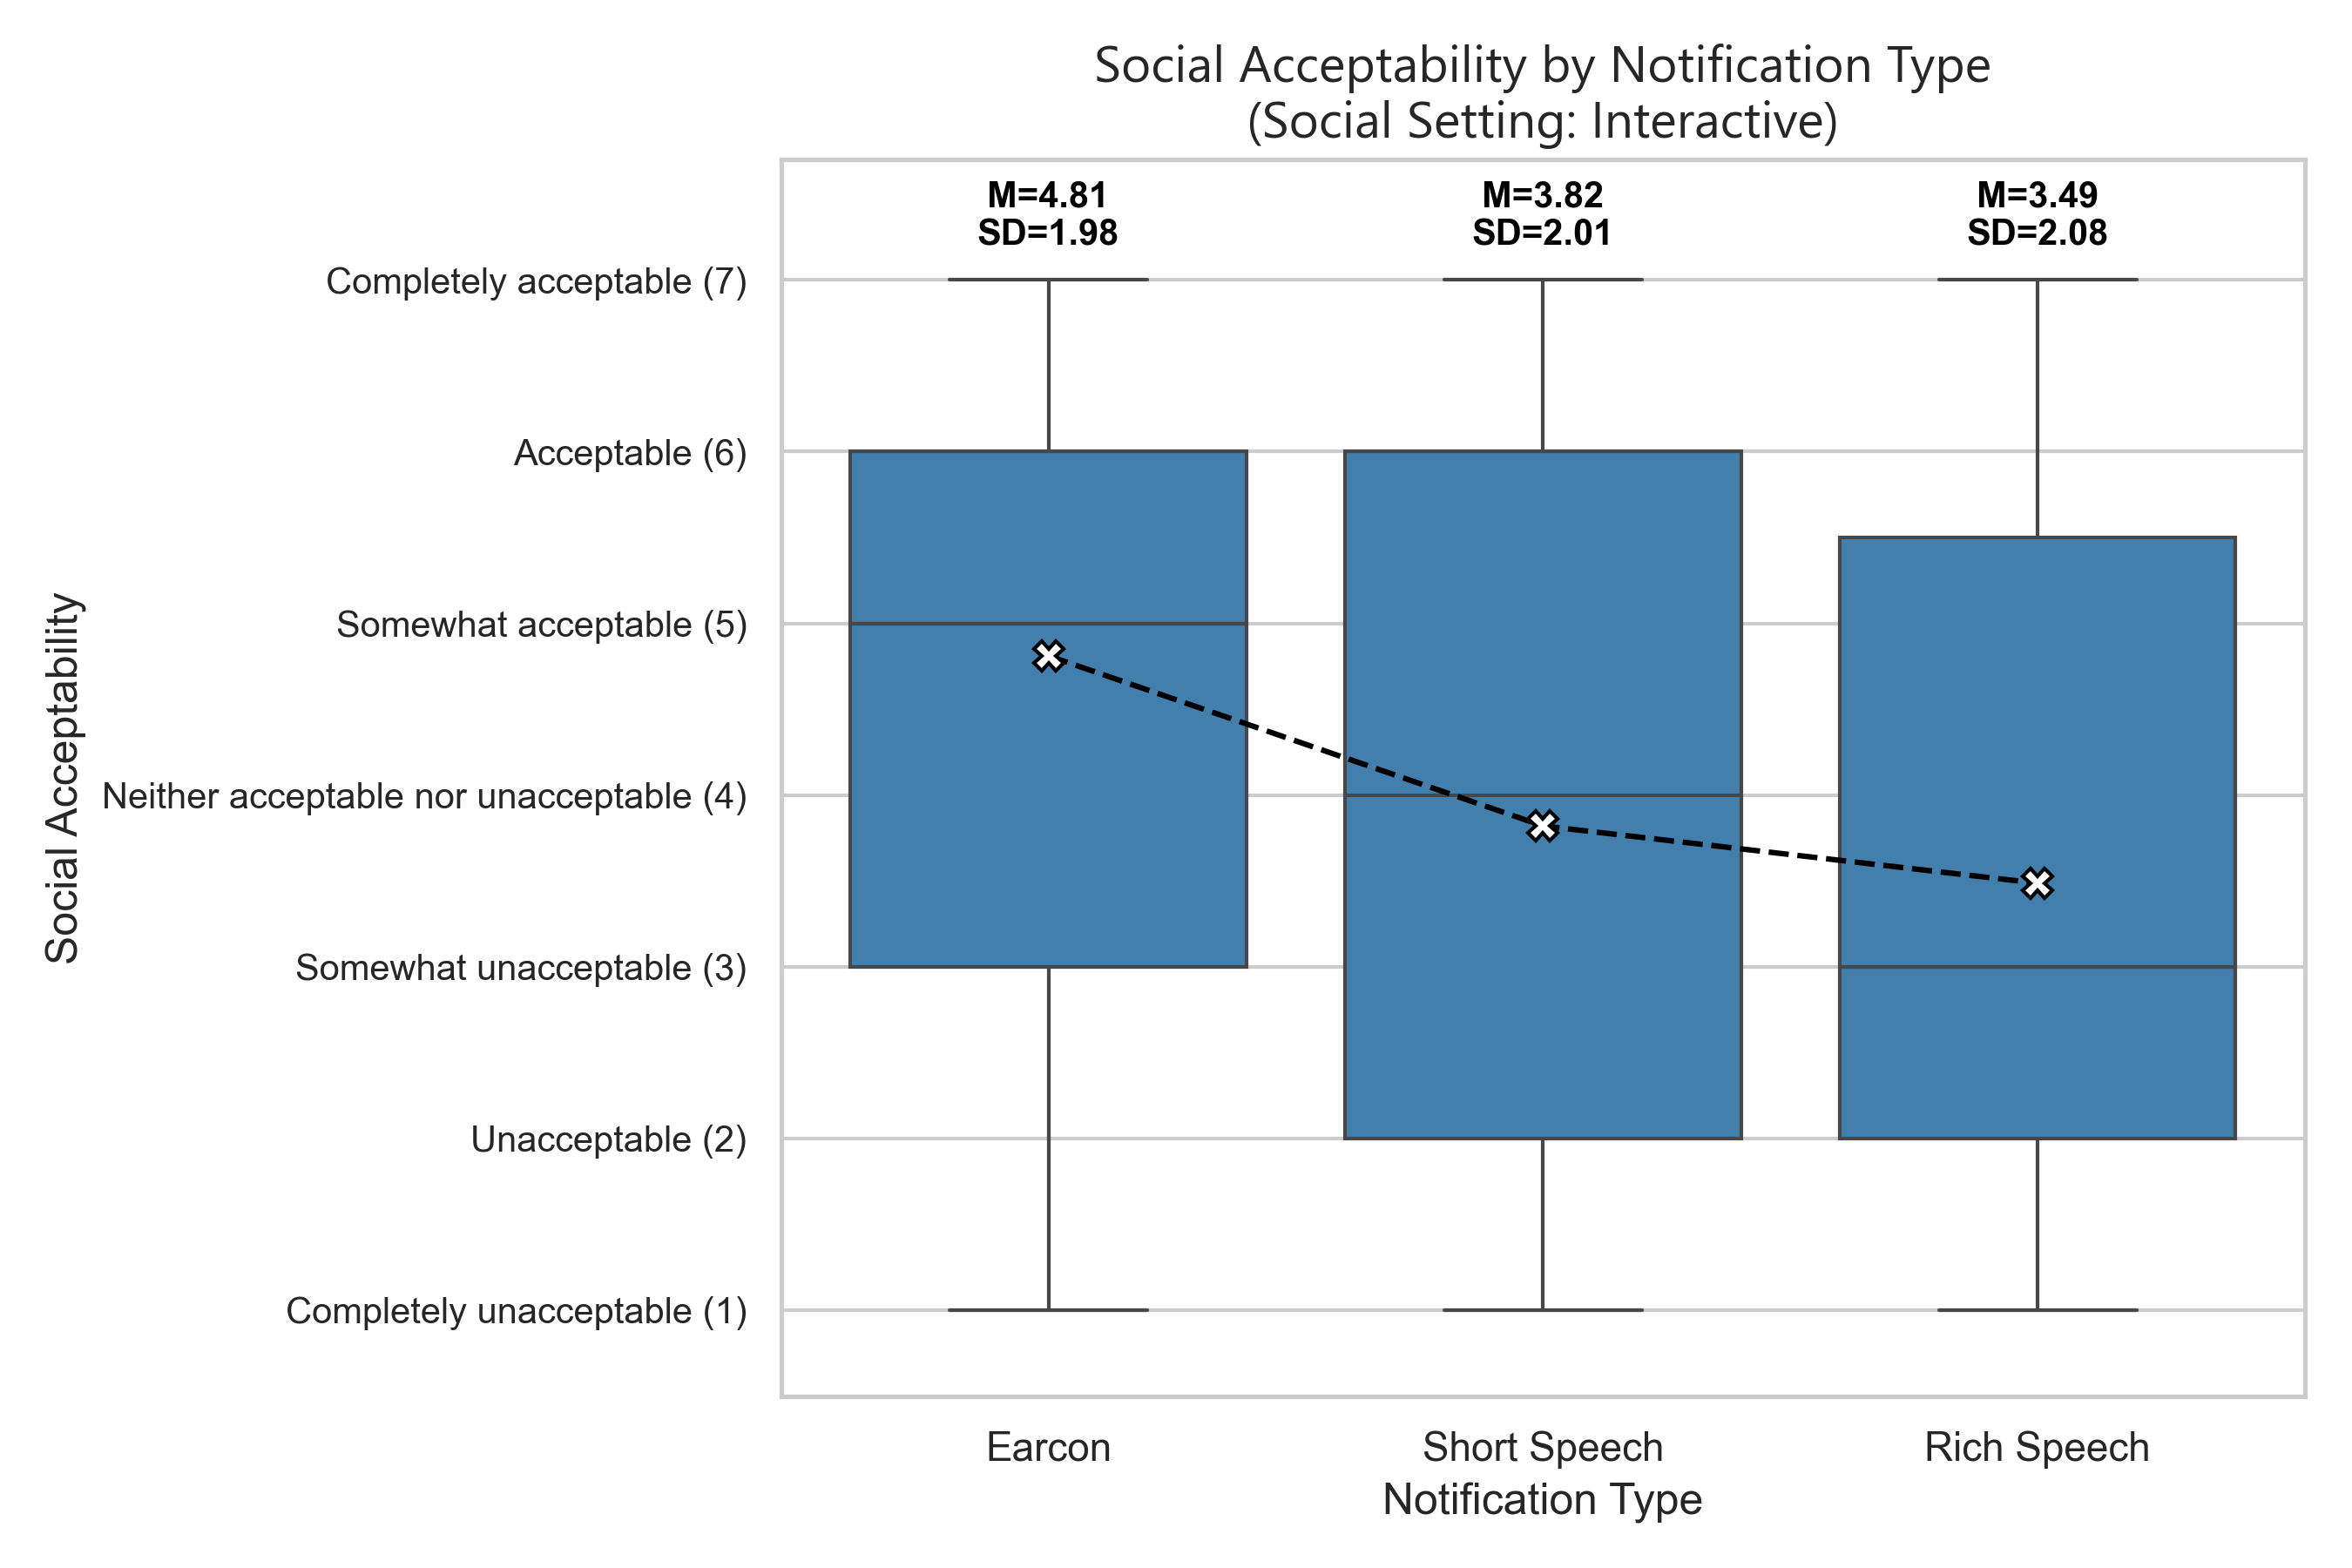
\includegraphics[width=\textwidth]{plots2/SocialAcceptability_Interactive.png}
        \caption{Interactive Co-Presence} % Dies ist Plot (e)
    \end{subfigure}
    \hfill
    \begin{subfigure}[b]{0.32\textwidth}
        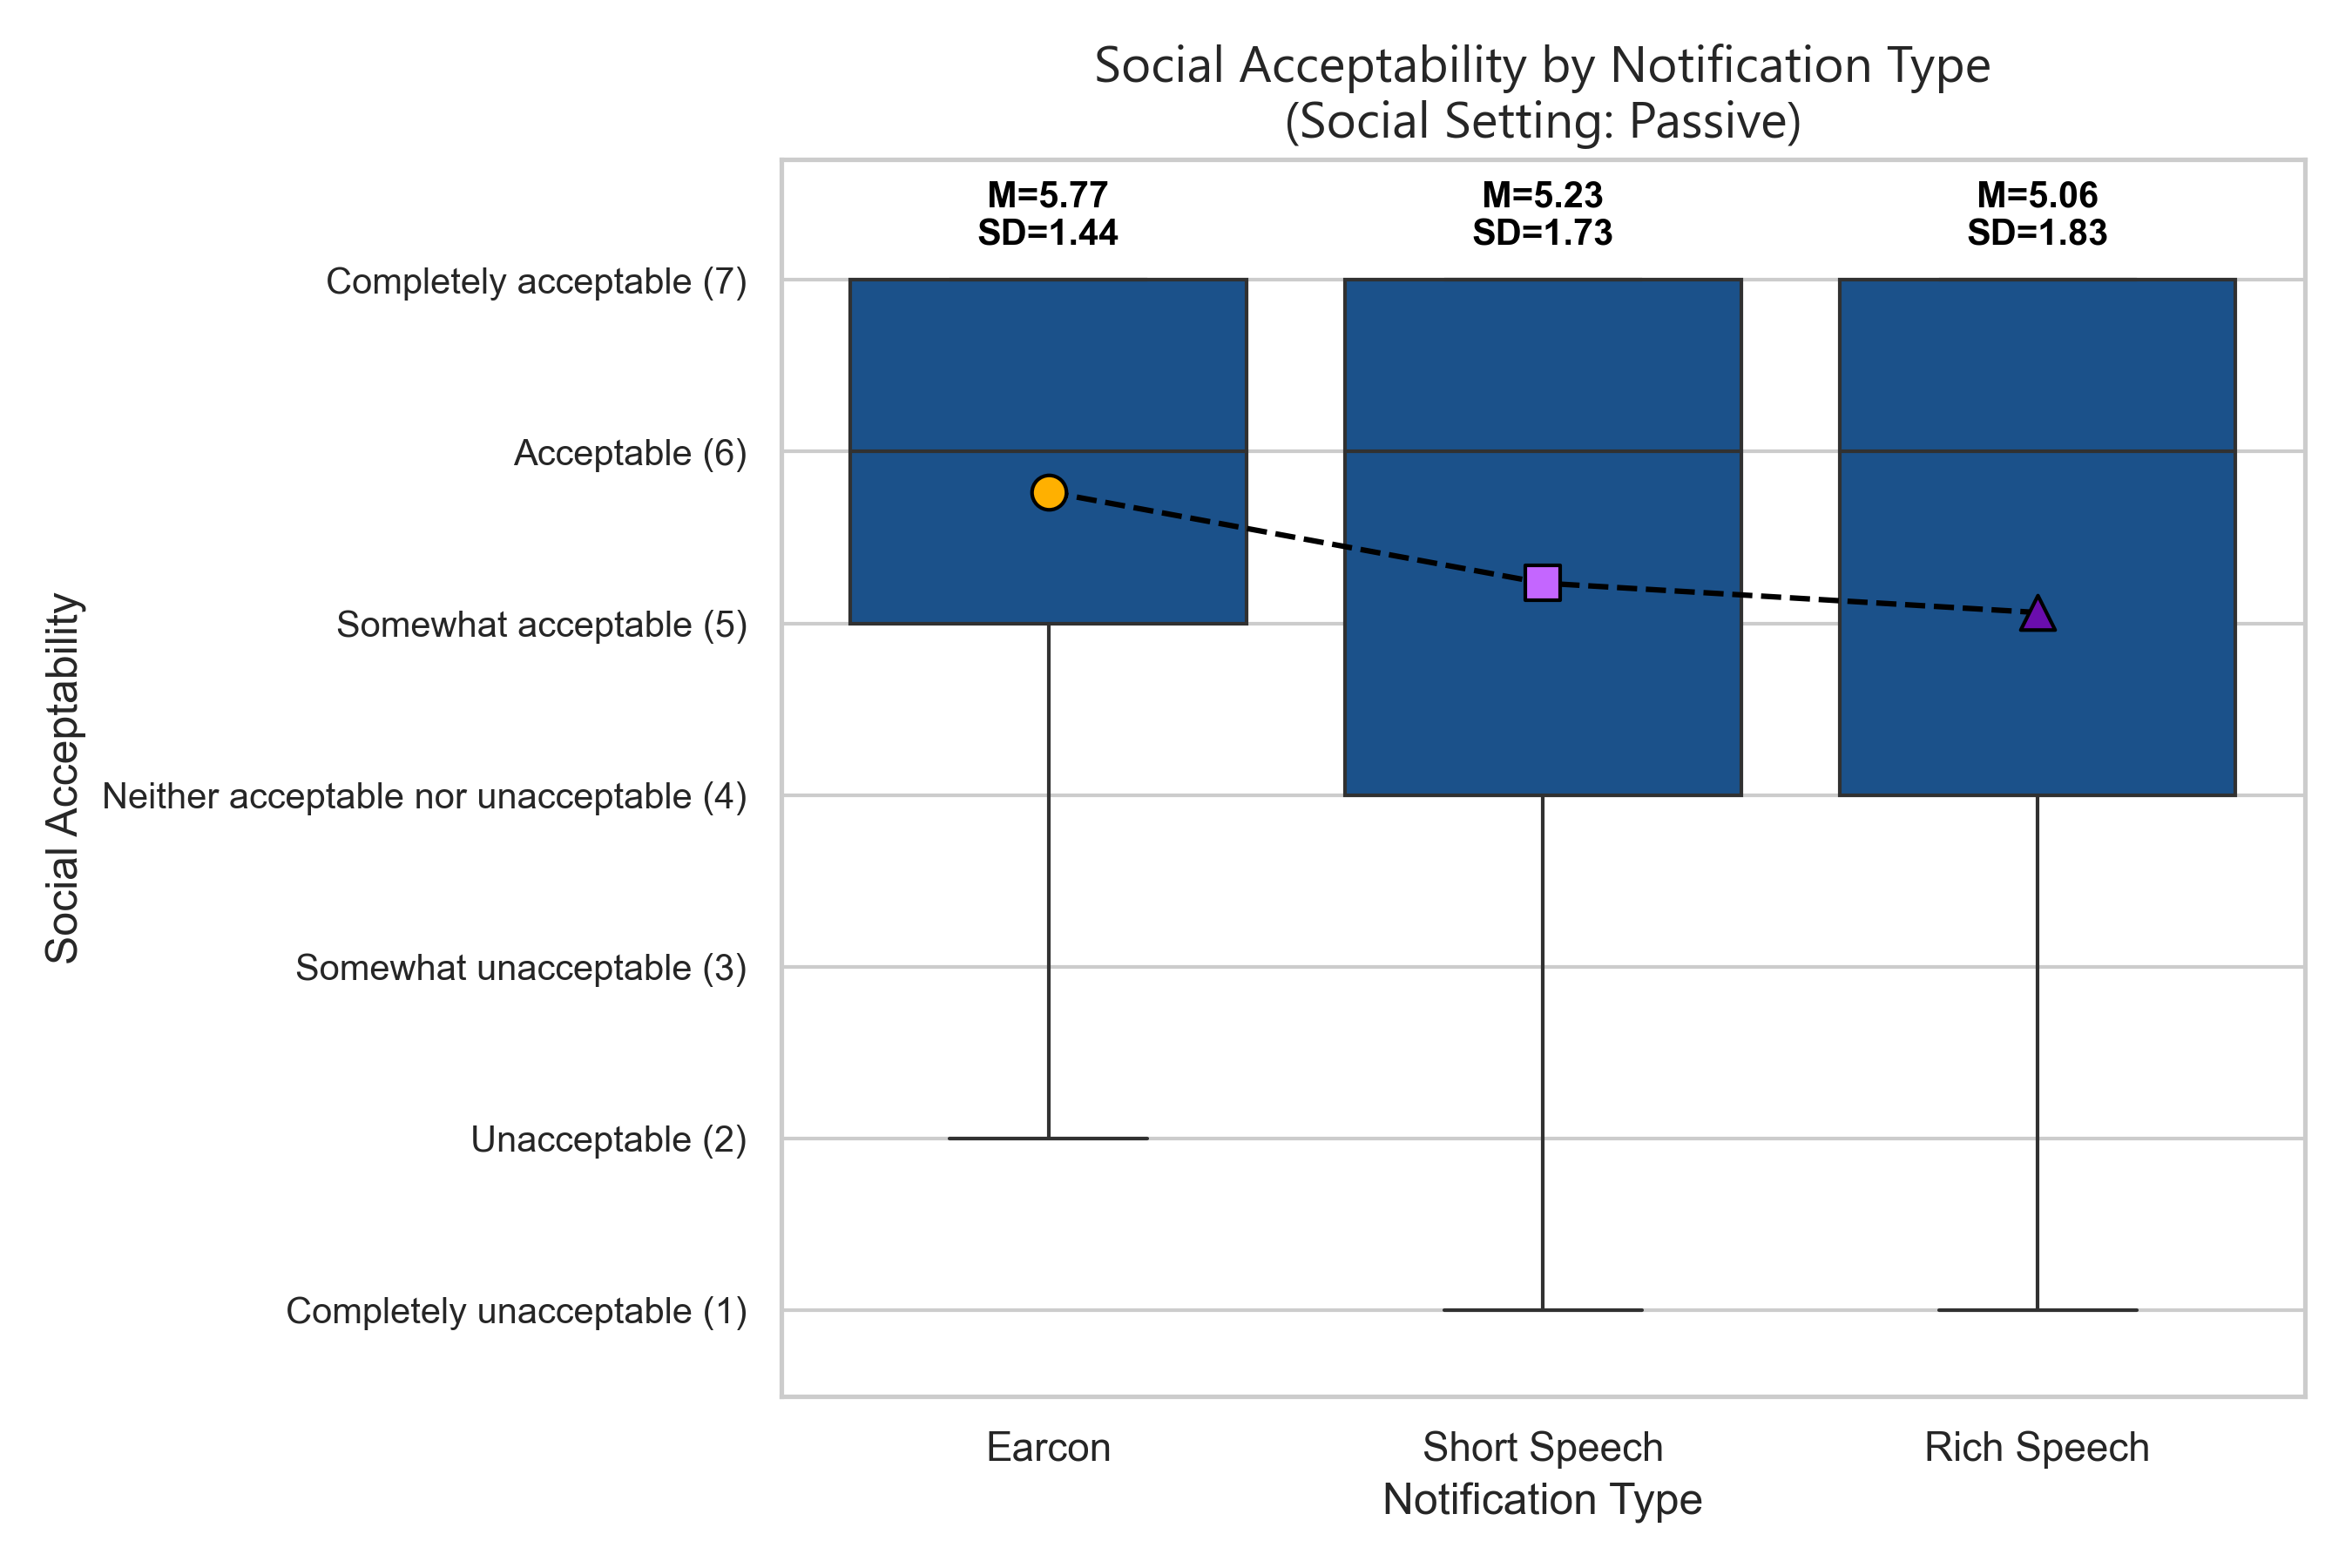
\includegraphics[width=\textwidth]{plots2/SocialAcceptability_Passive.png}
        \caption{Passive Co-Presence} % Dies ist Plot (d)
    \end{subfigure}

    \caption{Distribution of social acceptability scores. Plots (a) and (b) visualize the overarching main effects of social setting and notification type, corresponding directly to the marginal means derived from the Linear Mixed Model. Plots (c), (d), and (e) break down the social acceptability of each notification type across the three specific social settings.}
    \label{fig:box_social}
\end{figure}





\subsection{What Drives Detectability?}
\label{sec:res_detectability}
To analyze how well notifications could be perceived in various acoustic environments, we used the following model:
$$ \text{Detectability} \sim \text{Notification Type} + \text{Social Setting} + \text{Task Load} + \text{Soundscape} + (1 | \text{Participant}) $$

The physical acoustic environment predictably altered the user's ability to hear the notifications. Compared to environments with music ($M = 5.83$), completely quiet environments naturally improved detectability ($M = 6.44$; $\Delta M = 0.61, p < .001$), while background speech severely hindered it ($M = 5.41$; $\Delta M = -0.42, p < .001$), as seen in \autoref{fig:box_detectability}a. The contrast between quiet and speech environments was the largest observed effect ($\Delta M = -1.03, p < .001$), confirming that ambient speech represents the most challenging acoustic condition for notification perception.

We also found a significant effect regarding the notification type: \textit{Rich Speech} ($M = 6.01$) was significantly easier to detect overall than an abstract Earcon ($M = 5.74$; $\Delta M = 0.26, p = .007$). \autoref{fig:box_detectability}b details these findings across all notification formats.

Analyzing the interaction between soundscape and notification type reveals distinct auditory masking effects. In a completely quiet environment, all notification types are highly detectable (Earcon: $M = 6.21$; Rich Speech: $M = 6.59$). However, in an environment with background music, the Earcon becomes noticeably harder to detect ($M = 5.33$), while spoken notifications cut through the music more easily (Rich Speech: $M = 6.14$). Conversely, when the ambient soundscape consists of background speech, this effect reverses: the Earcon remains moderately detectable ($M = 5.69$), but the detectability of Short Speech ($M = 5.23$) and Rich Speech ($M = 5.31$) drops. This demonstrates that background speech directly masks incoming speech notifications, whereas music primarily masks abstract tonal alerts.

\begin{figure}[H]
    \centering
    % Obere Reihe: Main Effects
    \begin{subfigure}[b]{0.48\textwidth}
        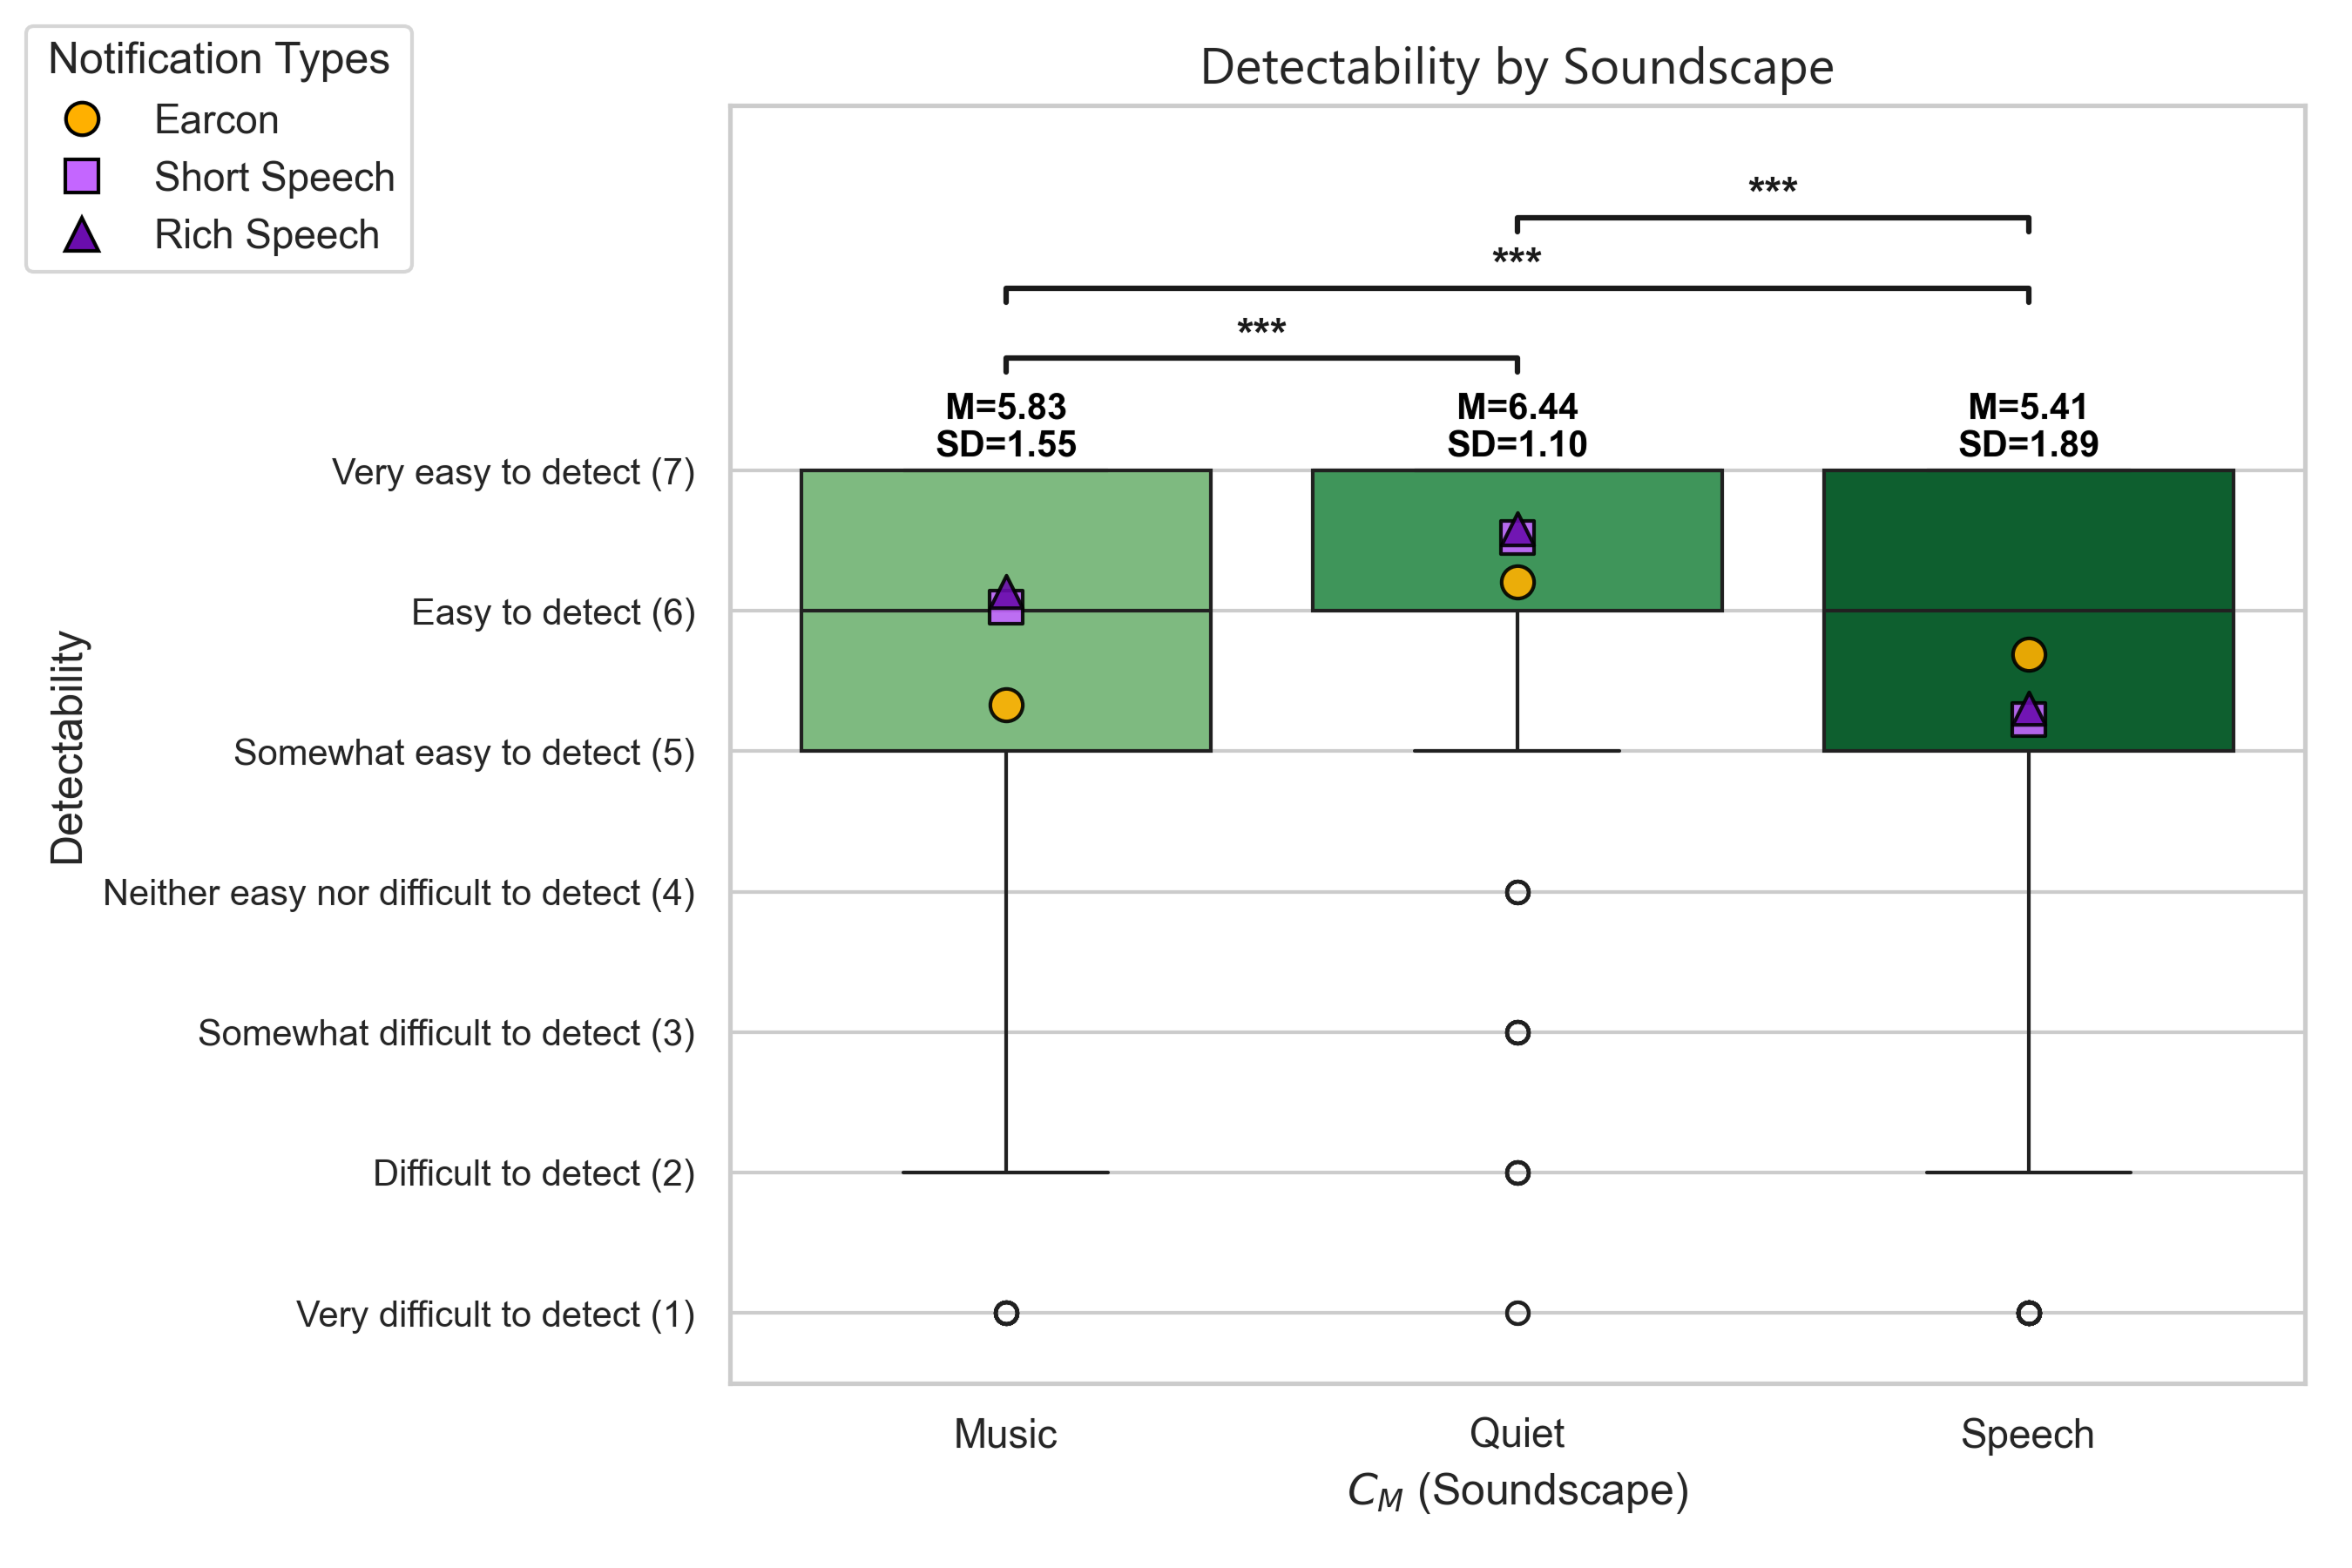
\includegraphics[width=\textwidth]{plots/PrimaryAdvanced_Overall_CM_vs_Detectability_inline.png}
        \caption{Overall by Soundscape}
    \end{subfigure}
    \hfill
    \begin{subfigure}[b]{0.48\textwidth}
        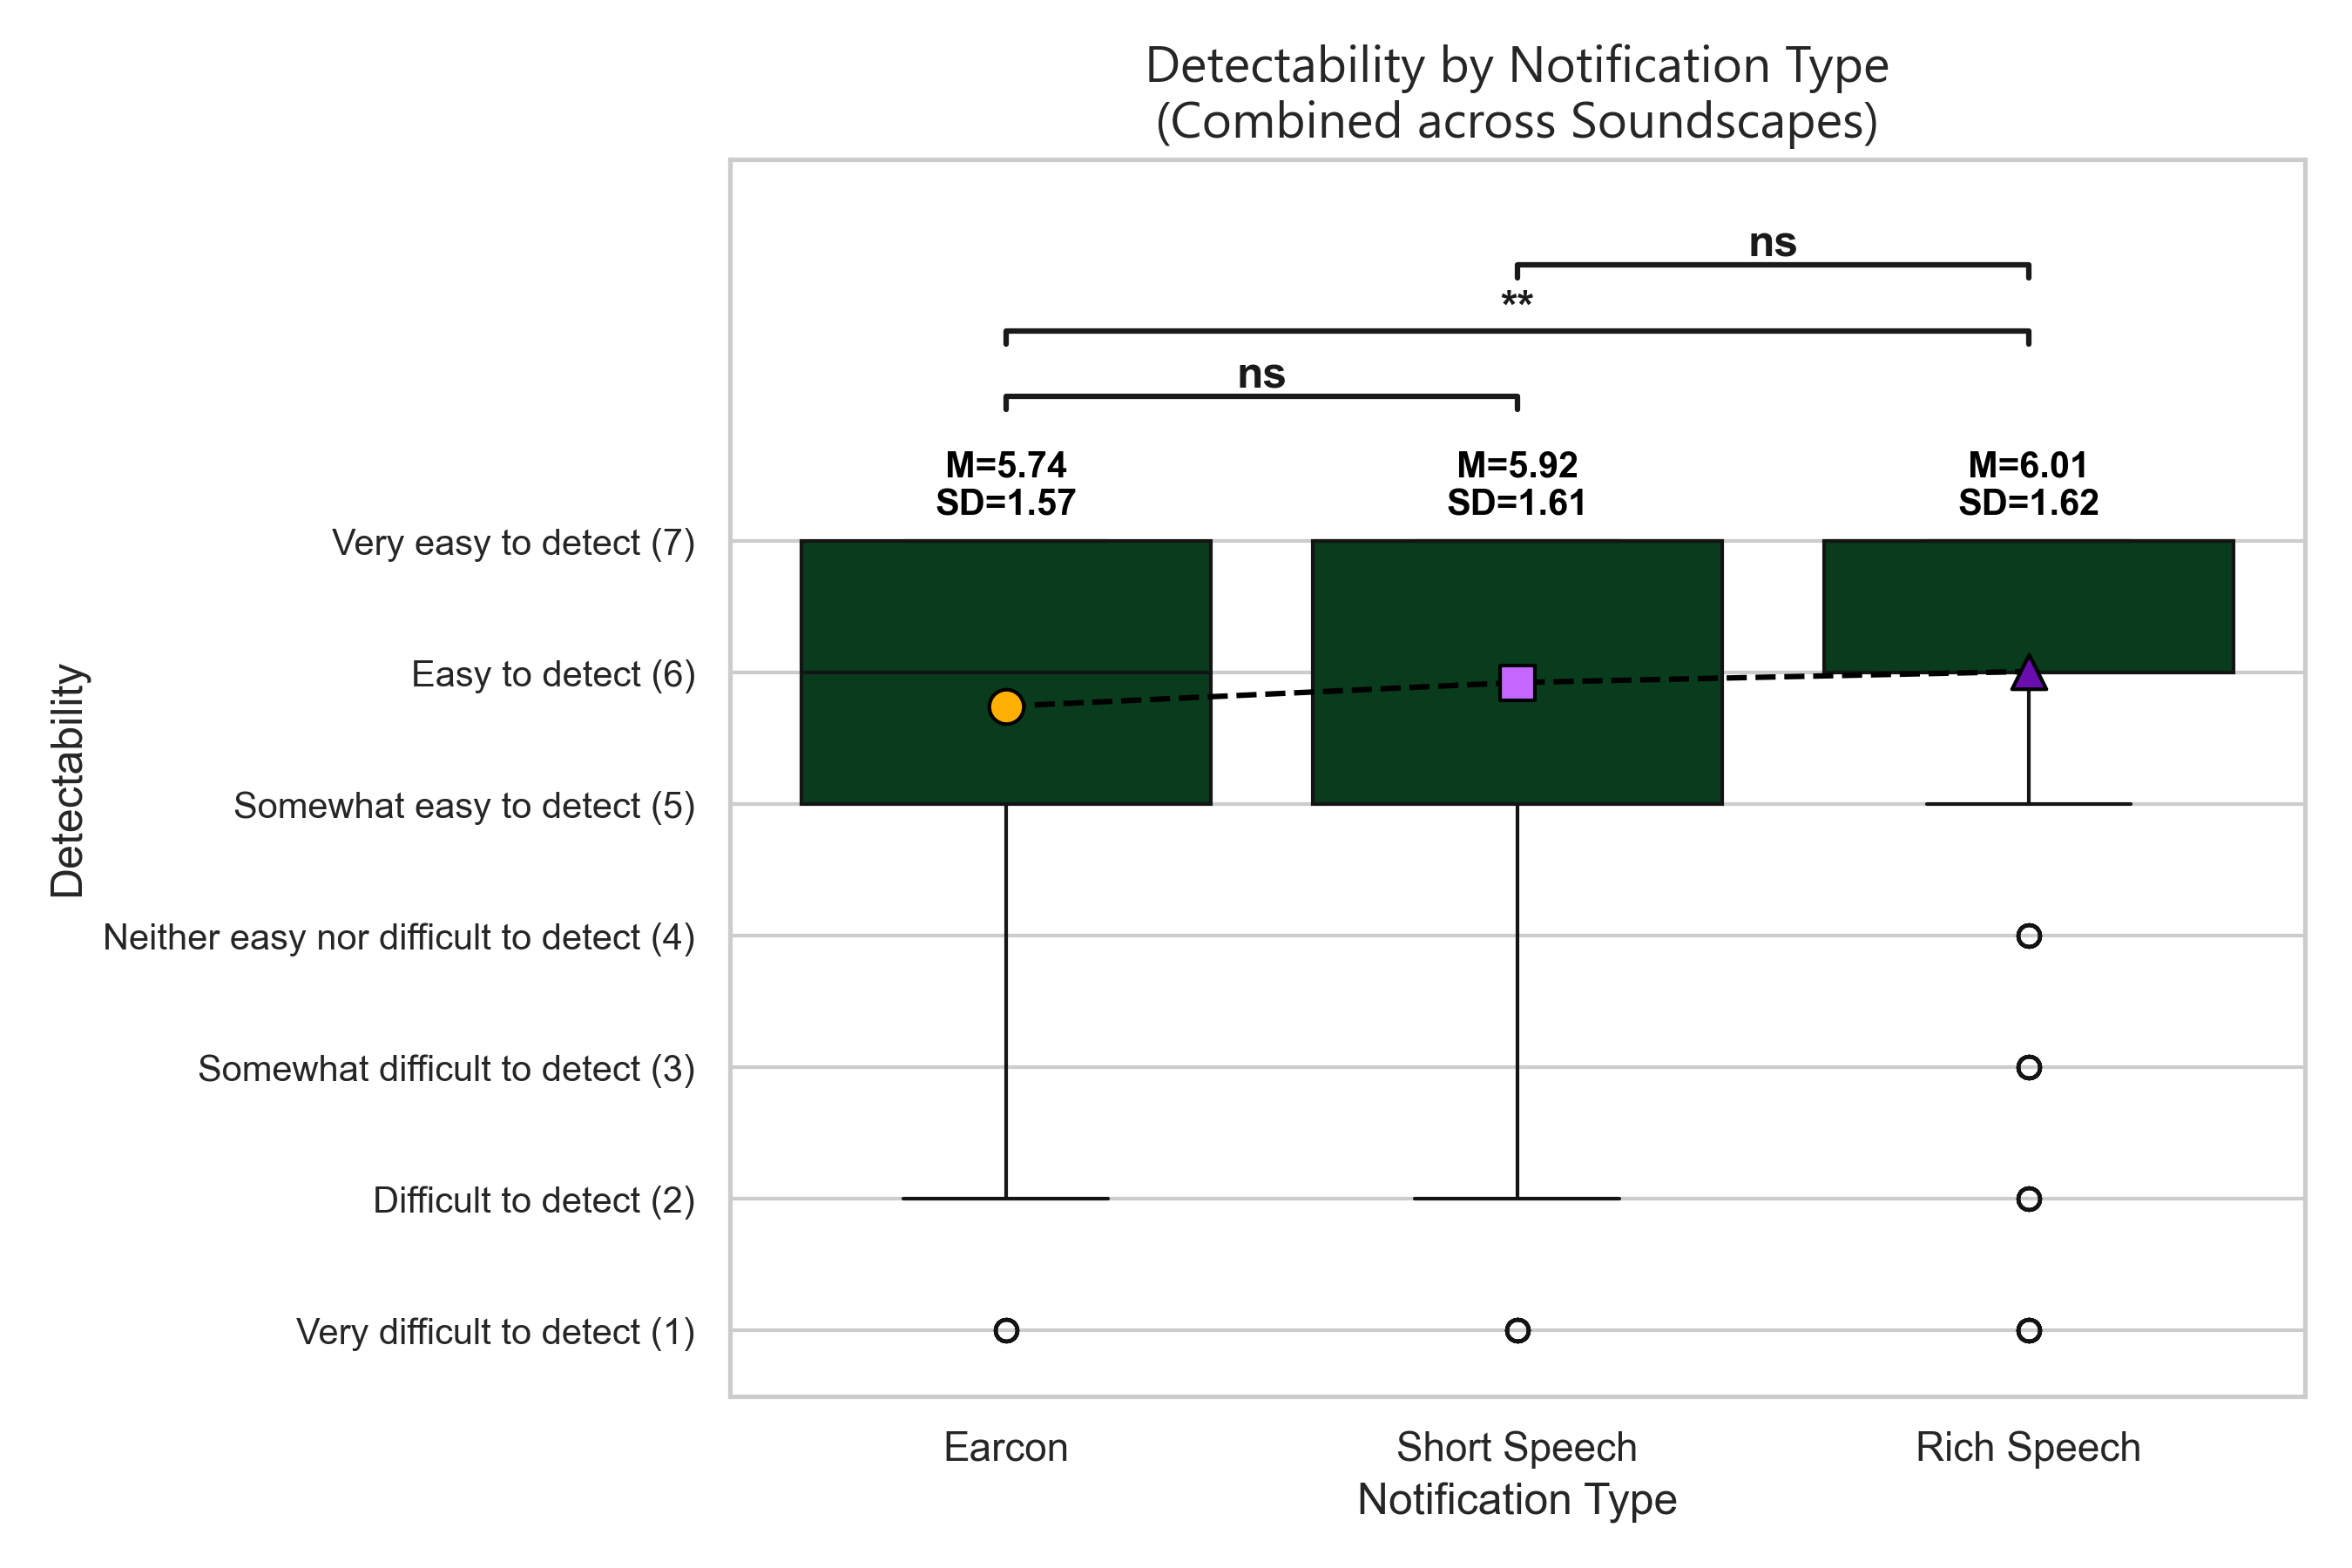
\includegraphics[width=\textwidth]{plots2/Detectability_Combined.png}
        \caption{Overall by Notification Type}
    \end{subfigure}
    
    \vskip\baselineskip % Abstand zwischen oberer und unterer Reihe
    
    % Untere Reihe: Breakdowns per Soundscape
    \begin{subfigure}[b]{0.32\textwidth}
        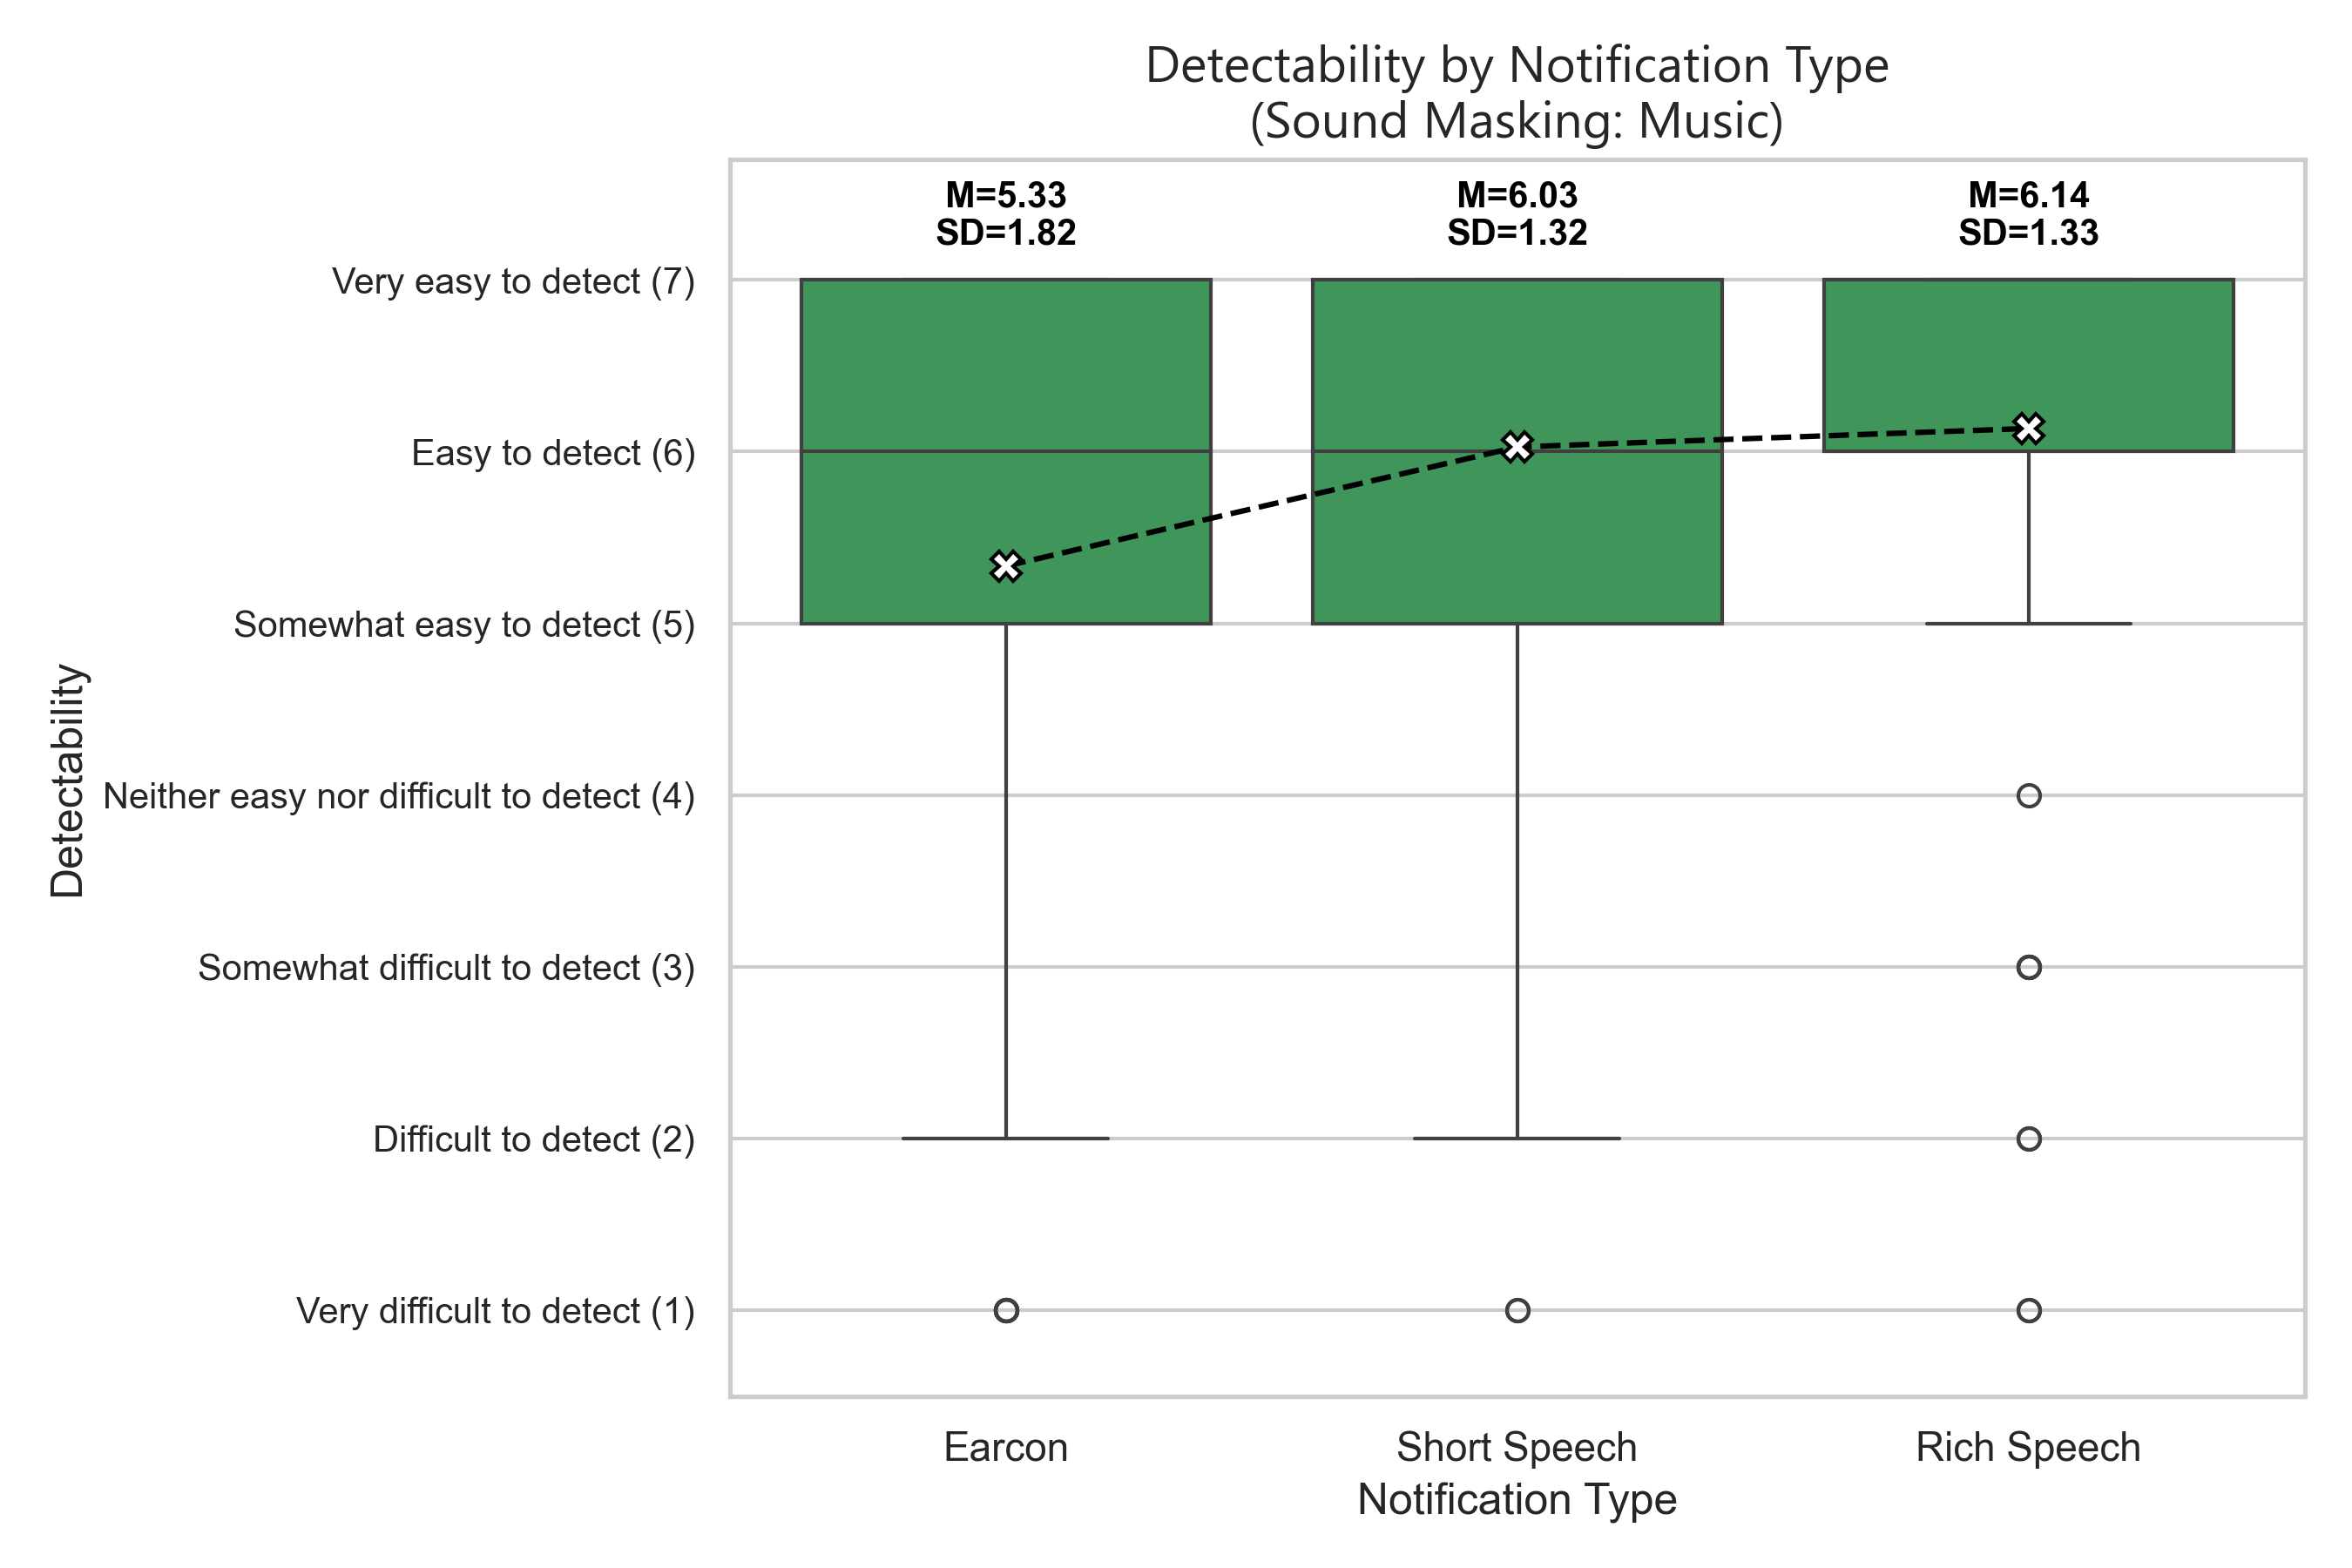
\includegraphics[width=\textwidth]{plots2/Detectability_Music.png}
        \caption{Music Environment}
    \end{subfigure}
    \hfill
    \begin{subfigure}[b]{0.32\textwidth}
        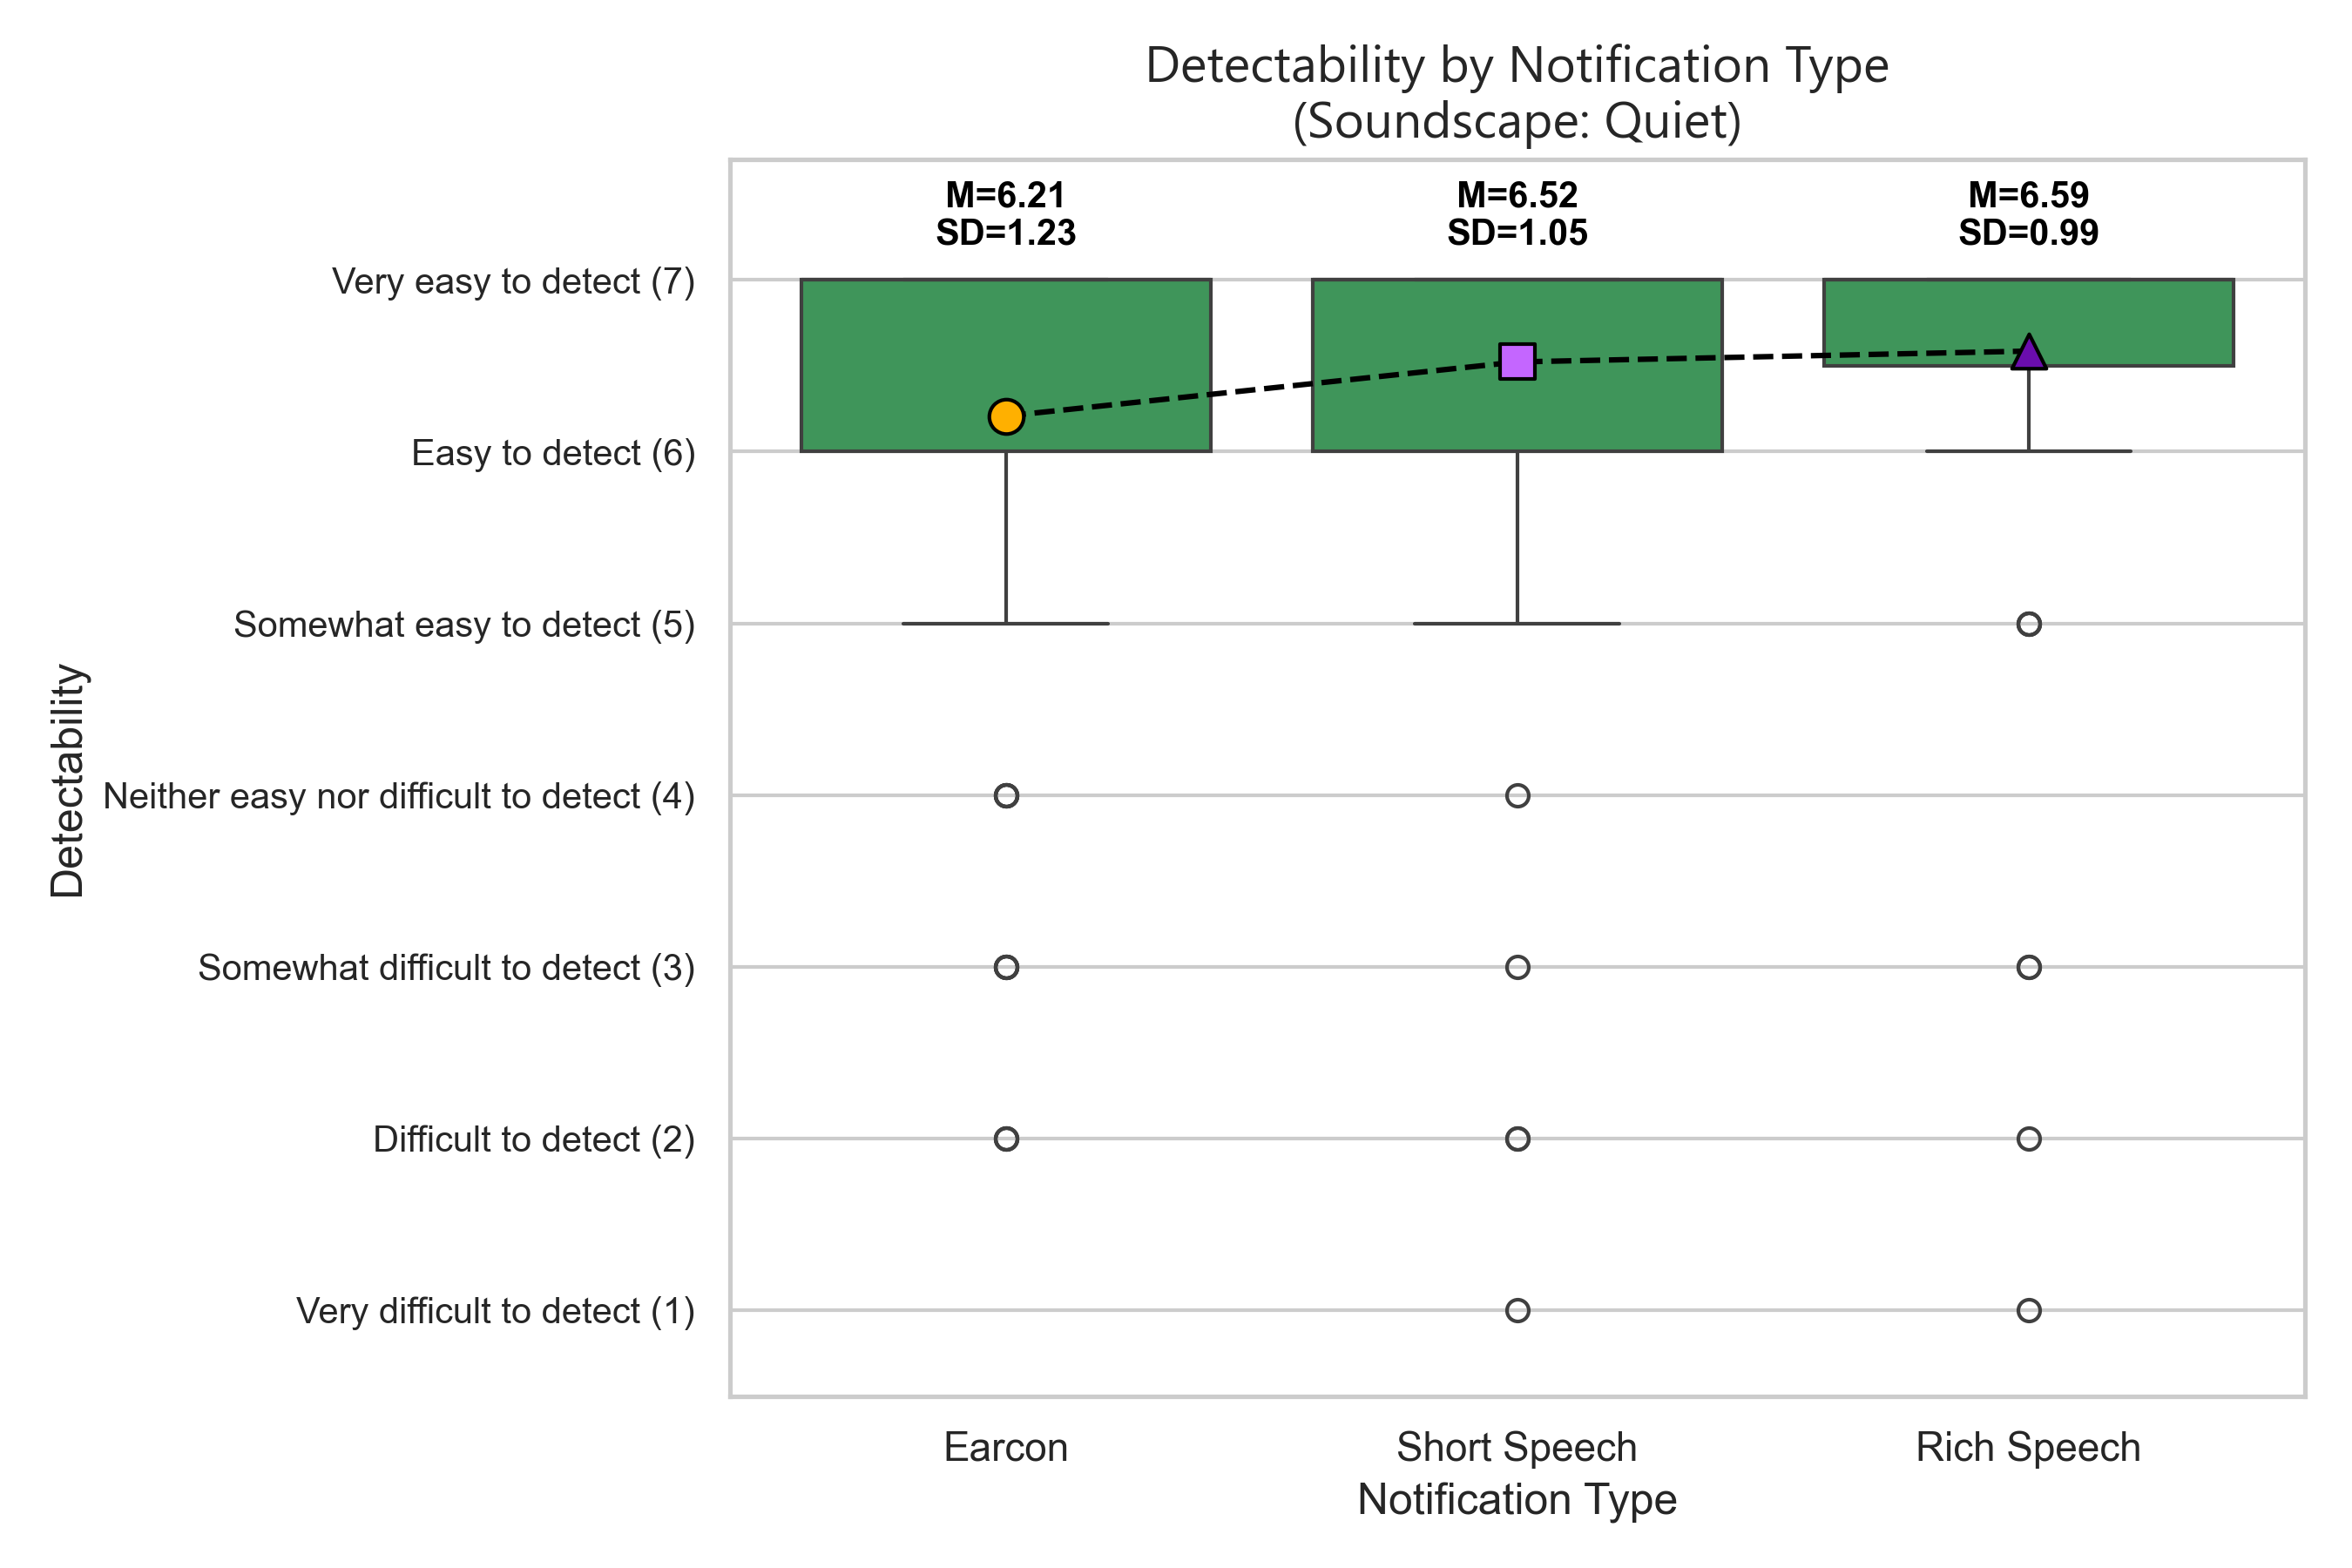
\includegraphics[width=\textwidth]{plots2/Detectability_Quiet.png}
        \caption{Quiet Environment}
    \end{subfigure}
    \hfill
    \begin{subfigure}[b]{0.32\textwidth}
        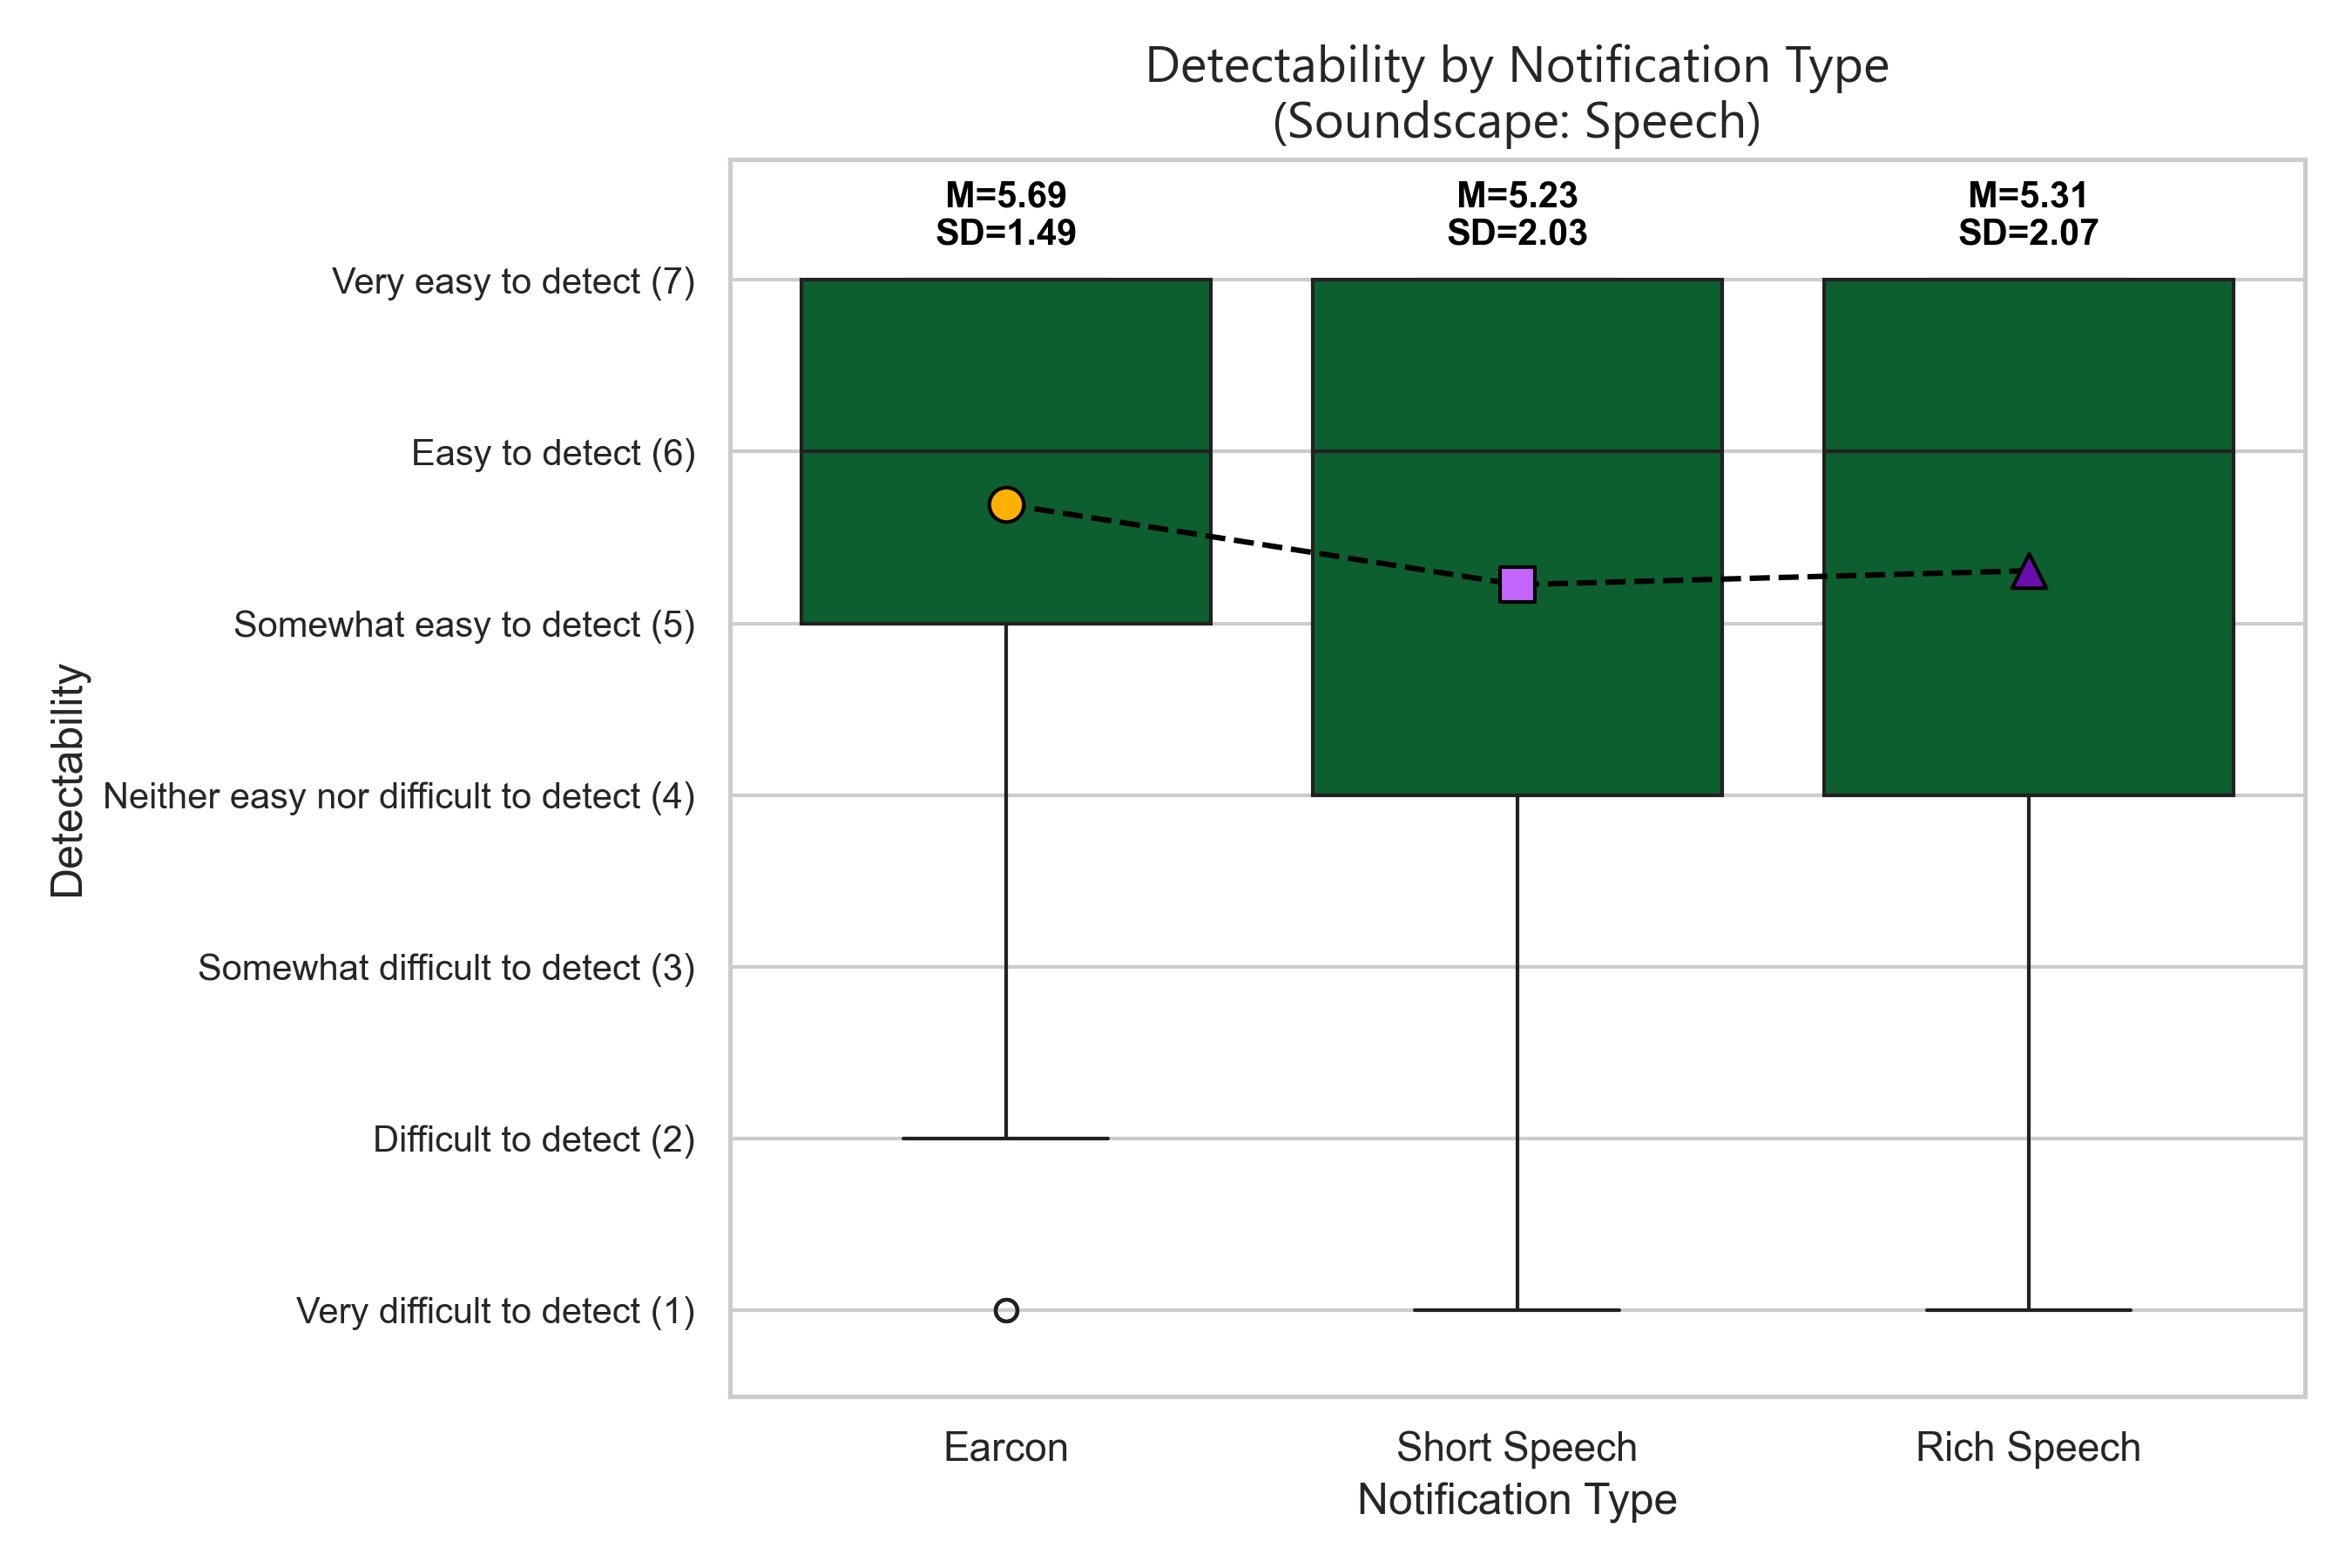
\includegraphics[width=\textwidth]{plots2/Detectability_Speech.png}
        \caption{Speech Environment}
    \end{subfigure}
    \caption{Detectability of notifications. Plots (a) and (b) visualize the overarching main effects of the soundscape and notification type, corresponding directly to the marginal means derived from the Linear Mixed Model. Plots (c), (d), and (e) break down the detectability of each notification type across the three specific acoustic environments.}
    \label{fig:box_detectability}
\end{figure}





\begin{comment}
\subsection{Understanding Appropriateness: A Synthesis}
\label{sec:res_appropriateness}

While the previous models describe how context shapes individual dimensions, they do not explain \textit{why} a user ultimately considers a notification "appropriate." To synthesize these findings, we fitted a fourth LMM predicting \textbf{Appropriateness} strictly based on the continuous ratings of Detectability, Disruption, and Social Acceptability, including their interactions to capture combined effects:

$$ \text{Appropriateness} \sim \text{Detectability} * \text{Disruption} * \text{Social Acceptability} + (1 | \text{Participant}) $$

Because this specific regression explores a single aggregated relationship rather than testing multiple parallel scenario factors, we evaluated it at the standard $\alpha = .05$ significance level.

The model revealed that \textbf{Social Acceptability} is the strongest driving factor for appropriateness ($\beta = 0.77, p < .001$). \textbf{Detectability} also played a significant, positive role ($\beta = 0.38, p = .036$). Crucially, \textbf{Disruption} alone was \textit{not} a significant baseline predictor of appropriateness ($\beta = 0.07, p = .677$), indicating that users do not inherently classify disruptive notifications as "inappropriate" if the message is urgent and important and the social context permits.

To translate these findings into actionable system parameters for the SonoAdapt architecture, we performed a Dominance Analysis (Relative Importance Analysis). While $\beta$ coefficients indicate the direction and magnitude of an effect, dominance analysis partitions the total variance explained by the model ($R^2$) to determine the exact percentage of influence each factor wields over the user's final appropriateness decision.

\begin{table}[H]
\centering
\caption{Relative Importance Analysis determining the percentage of influence each dimension has on the overall Appropriateness rating. These normalized weights serve as the foundational parameters for the SonoAdapt utility function.}
\label{tab:relative_importance}
\begin{tabular}{@{}lcc@{}}
\toprule
\textbf{Predictor} & \textbf{Relative Importance (Normalized)} & \textbf{Percentage of Influence} \\
\midrule
Social Acceptability & 0.527 & 52.7\% \\
Disruption & 0.451 & 45.1\% \\
Detectability & 0.021 & 2.1\% \\
\bottomrule
\end{tabular}
\end{table}

As shown in \autoref{tab:relative_importance}, Social Acceptability (52.7\%) and Disruption (45.1\%) overwhelmingly dominate the appropriateness construct. Detectability (2.1\%) contributes marginally to the variance, suggesting a threshold effect: as long as a notification is audible, its exact degree of salience matters far less than its social and cognitive impact. Consequently, these empirically derived weights ($w_a \approx 0.53$, $w_e \approx 0.45$, $w_l \approx 0.02$) directly inform the cost-calculation parameters within the SonoAdapt utility optimization framework.
\end{comment}
\subsection{Understanding Appropriateness: A Synthesis}
\label{sec:res_appropriateness}

While the previous models describe how context shapes individual dimensions, they do not explain \textit{why} a user ultimately considers a notification "appropriate." To synthesize these findings, we fitted a fourth LMM predicting \textbf{Appropriateness} strictly based on the continuous ratings of Detectability, Disruption, and Social Acceptability:

$$ \text{Appropriateness} \sim \text{Detectability} + \text{Disruption} + \text{Social Acceptability} + (1 | \text{Participant}) $$

Because this specific regression explores a single aggregated relationship rather than testing multiple parallel scenario factors, we evaluated it at the standard $\alpha = .05$ significance level.

The model revealed that all three dimensions are highly significant predictors of appropriateness. \textbf{Social Acceptability} serves as the strongest positive driving factor ($\beta = 0.53, p < .001$). \textbf{Disruption} also heavily impacts appropriateness, but in the opposite direction: as expected, higher perceived disruption significantly decreases the likelihood of a notification being deemed appropriate ($\beta = -0.38, p < .001$). Finally, \textbf{Detectability} plays a smaller, yet significant positive role ($\beta = 0.12, p < .001$).

To translate these findings into actionable system parameters for the SonoAdapt architecture, we performed a Dominance Analysis (Relative Importance Analysis). While $\beta$ coefficients indicate the direction and magnitude of an effect, dominance analysis partitions the total variance explained by the model ($R^2$) to determine the exact percentage of influence each factor wields over the user's final appropriateness decision.

\begin{table}[H]
\centering
\caption{Relative Importance Analysis determining the percentage of influence each dimension has on the overall Appropriateness rating. These normalized weights serve as the foundational parameters for the SonoAdapt utility function.}
\label{tab:relative_importance}
\begin{tabular}{@{}lcc@{}}
\toprule
\textbf{Predictor} & \textbf{Relative Importance (Normalized)} & \textbf{Percentage of Influence} \\
\midrule
Social Acceptability & 0.527 & 52.7\% \\
Disruption & 0.451 & 45.1\% \\
Detectability & 0.021 & 2.1\% \\
\bottomrule
\end{tabular}
\end{table}

As shown in \autoref{tab:relative_importance}, Social Acceptability (52.7\%) and Disruption (45.1\%) overwhelmingly dominate the appropriateness construct. Detectability (2.1\%) contributes marginally to the variance, suggesting a threshold effect: as long as a notification is audible, its exact degree of salience matters far less than its social and cognitive impact. Consequently, these empirically derived weights ($w_a \approx 0.53$, $w_e \approx 0.45$, $w_l \approx 0.02$) directly inform the cost-calculation parameters within the SonoAdapt utility optimization framework.







\subsection{Summary of Descriptive Statistics}
\label{sec:res_summary_table}
To provide a comprehensive overview of the context-dependent shifts in user perception, \autoref{tab:descriptive_summary} summarizes the aggregated mean scores across all primary relationships investigated in this study. The table juxtaposes the three notification types against the specific environmental factors (Task Load, Social Setting, and Soundscape) that drive the respective dimensions of Disruption, Social Acceptability, and Detectability.

\begin{table}[H]
\centering
\caption{Summary of descriptive mean scores ($M$) for each notification type, isolated by the contextual factors relevant to our primary hypotheses. All ratings are based on 7-point Likert scales (1 = lowest/worst, 7 = highest/best).}
\label{tab:descriptive_summary}
\resizebox{\textwidth}{!}{%
\begin{tabular}{@{}l ccc c ccc c ccc@{}}
\toprule
 & \multicolumn{3}{c}{\textbf{Disruption}} & & \multicolumn{3}{c}{\textbf{Social Acceptability}} & & \multicolumn{3}{c}{\textbf{Detectability}} \\
 & \multicolumn{3}{c}{(by Task Load)} & & \multicolumn{3}{c}{(by Social Setting)} & & \multicolumn{3}{c}{(by Soundscape)} \\
\cmidrule{2-4} \cmidrule{6-8} \cmidrule{10-12}
\textbf{Notification Type} & Low & High Mental & High Physical & & Alone & Passive & Interactive & & Quiet & Music & Speech \\
\midrule
\textbf{Earcon}       & 2.55 & 4.05 & 2.80 & & 5.87 & 5.77 & 4.81 & & 6.21 & 5.33 & 5.69 \\
\textbf{Short Speech} & 3.86 & 5.29 & 3.68 & & 5.52 & 5.23 & 3.82 & & 6.52 & 6.03 & 5.23 \\
\textbf{Rich Speech}  & 4.37 & 5.66 & 4.09 & & 5.33 & 5.06 & 3.49 & & 6.59 & 6.14 & 5.31 \\
\bottomrule
\end{tabular}%
}
\end{table}





\subsection{Overall Preferences}

\subsubsection{User Preference for Type}
\label{sec:user_preference_type}

In each of the nine scenarios, participants were asked to state their overall preference for the auditory notification type (Earcon, Short Speech, Rich Speech, or No Audio) after experiencing all variations. This initial in-scenario choice was made independently of any potential delivery delay, forcing users to evaluate the format based solely on the immediate scenario they experienced. 

\autoref{fig:preference_flow} illustrates the evolution of user preferences across three stages of the survey. Stage 1 represents the users' baseline preference for an important and urgent message, independent of any specific scenario (as previously discussed in \autoref{sec:speech_notification} and \autoref{fig:general_notification_preference}). Stage 2 shows the aggregated preferences when users were immersed in the specific scenarios. \\
Interestingly, when confronted with the realities of the scenario, the overall preference for speech-based notifications dropped from 72.9\% (baseline) to 45.6\%. Conversely, the preference for abstract Earcons increased from 10.8\% to 32.7\%, indicating that environmental constraints inherently make users more cautious about receiving spoken information.

\begin{figure}[H]
    \centering
    
\includegraphics[width=0.9\textwidth]{plots3/06_Preference_Development_Flow.png}
    \caption{Evolution of notification format preferences. The chart demonstrates how the initial baseline preference for speech (Stage 1) drops when forced into immediate contextual scenarios (Stage 2), but rebounds when users are allowed to choose an appropriate delivery timing (Stage 3).}
    \label{fig:preference_flow}
\end{figure}

To further understand how specific combinations of context drove these decisions, \autoref{fig:preference_matrix} breaks down the preferred types across all nine scenarios of Stage 2. The matrix highlights the underlying environmental variables (Social Setting, Task Load, and Soundscape) alongside the top two qualitative reasons driving the participants' choices in each specific situation.

\begin{figure}[H]
    \centering
    \includegraphics[width=0.95\textwidth]{plots3/PreferenceMatrix.png}
    \caption{Scenario preference matrix detailing the notification choices in Stage 2 across the nine evaluated scenarios, including the primary qualitative reasons provided by participants.}
    \label{fig:preference_matrix}
\end{figure}

Crucially, participants were subsequently asked to choose their preferred \textit{timing} within the scenario, and then select their preferred notification type based on that specific delivery window. When participants were given the agency to shift the notification to an appropriate moment, the preference for speech-based notifications rebounded to 70.2\% (Stage 3 in \autoref{fig:preference_flow}), closely mirroring their original, context-independent baseline. 

Equally revealing is the behavior of the ``No Audio'' and Earcon categories between Stage 2 and Stage 3. In Stage 2, selecting ``No Audio'' (21.6\%) functioned largely as a proxy for a manual delay, a way for users to reject an interruption at a highly inappropriate moment. Once users were granted explicit control over timing in Stage 3, the need to completely mute the system nearly vanished (dropping to just 1.5\%). However, instead of universally defaulting to speech, many of these users shifted to Earcons, keeping the Earcon preference notably high at 28.2\% (compared to its 10.8\% baseline in Stage 1). This retention highlights a critical reality of contextual adaptation: delaying a notification changes the \textit{cognitive} load, but it rarely changes the \textit{physical} environment. For instance, waiting for a ``natural pause'' in a team meeting or taking a sip of coffee in a café still leaves the user surrounded by others. In these persistent social or public contexts, Earcons act as a safe, privacy-preserving compromise. They serve as a cognitive bookmark that subtly alerts the user without the social awkwardness of broadcasting a personal message.

This behavioral shift clearly demonstrates that users generally want to receive urgent and important notifications via speech, provided the context permits it. When the immediate environment is hostile to spoken audio (e.g., the soundscape already contains competing speech or the user is in an active conversation), participants initially opt for Earcons or No Audio. However, by leveraging intelligent timing delays to wait for a natural break, system designs can safely deliver the higher-information speech formats that users inherently prefer, while continuing to utilize Earcons as a robust fallback when social or environmental constraints persist.






\subsubsection{User Preference for Timing}
\label{sec:user_preference_timing}

To understand exactly \textit{when} users preferred to receive an important and urgent notification, we aggregated their chosen delivery timings across all nine scenarios (see Figure \ref{fig:overall_timing_pref}).\footnote{Note: Participants who selected ``Other'' provided open-text reasoning. These responses were qualitatively reviewed and merged into the four standardized timeline categories, as they universally described variations of these distinct pauses rather than entirely new timing concepts.} 

Overall, immediate delivery was the single most preferred option, accounting for 45.6\% ($n=152$) of the responses. However, this means that the majority of the time (54.4\% combined), participants opted to defer the notification. When delaying, users most frequently waited until the ``After Task is Finished'' phase (28.2\%, $n=94$), followed by taking a ``Micro-Break Within Task'' (16.2\%, $n=54$), and finally a ``Break Between Subtasks'' (9.9\%, $n=33$). 

\begin{figure}[H]
    \centering
    
\includegraphics[width=0.6\textwidth]{plots3/02_Overall_Timing_Preference.png}
    \caption{Overall timing preference aggregated across all 9 scenarios.}
    \label{fig:overall_timing_pref}
\end{figure}

While these aggregated totals show a general willingness to delay, they mask the highly context-dependent nature of these decisions. To uncover this, we mapped the flow of timing preferences scenario-by-scenario, grouping the three delay stages into a single ``Total Delayed'' metric to compare against the ``Immediate'' baseline (see Figure \ref{fig:preference_matrix_time}). Although participants did not physically experience the delayed deliveries in the study but choosing them hypothetically via multiple-choice, this aggregated data reveals a crucial interaction between \textit{when} a notification is delivered and \textit{what} format is preferred.

In highly demanding or acoustically restrictive environments, users are forced to make a trade-off between the immediacy of the notification and the amount of information they can comfortably receive. For example, in Scenario 3 (Cooking Dinner with a podcast playing), the acoustic constraint of the background speech makes an immediate spoken notification highly disruptive. Consequently, when people had to choose an overall preferred version in this exact moment the unobtrusive \textit{Earcon} was the top choice (\autoref{fig:preference_matrix}). However, when participants were allowed to choose a timing they delayed the notification to a natural pause (e.g., a break in the podcast or while waiting for water to boil), the top format preference shifted overwhelmingly to \textit{Rich Speech}. A similar pattern emerged in Scenario 1 (Coding alone): immediate delivery favored \textit{Short Speech}, but delaying the notification allowed users to comfortably accept \textit{Rich Speech}.

\begin{figure}[H]
    \centering
    \includegraphics[width=\textwidth]{plots3/PreferenceMatrixTime.png}
    \caption{Scenario-by-scenario flow of timing preferences. The green highlighted boxes indicate whether the majority of users preferred Immediate delivery or a Delayed delivery, alongside the most preferred audio format for that choice.}
    \label{fig:preference_matrix_time}
\end{figure}

These behavioral shifts provide the foundational design directive for \textit{SonoAdapt}. It demonstrates that users generally prefer the high information density of speech for urgent messages, but are often prevented from receiving it due to momentary environmental constraints. Therefore, an intelligent adaptive system should not simply default to muting the device or playing an Earcon when the current context is inappropriate. Instead, the system must balance format and time: if it can anticipate an appropriate pause in the near future (such as an imminent micro-break), it can delay the delivery and ``upgrade'' the notification to the globally preferred Rich Speech. Conversely, if a suitable pause is too far in the future and the message urgency dictates immediate delivery, the system must ``downgrade'' to an Earcon to safely alert the user without causing severe disruption.




\subsubsection{Intra-User Variance: Adaptability of Type}
\label{sec:intra_user_variance_type}


Beyond evaluating each notification type on individual Likert scales, analyzing participants' discrete choices across all nine scenarios allowed us to measure \textit{intra-user variance}. This metric essentially captures whether individual participants stuck to a single ``favorite'' setting globally, or if they actively adapted their preferences to fit the changing environmental context. 

As illustrated in \autoref{fig:variance_format}, participants strongly reject a static, ``one-size-fits-all'' notification type. In their immediate in-scenario evaluations (Stage 2), 89.2\% of users changed their preferred audio format at least once. Only 10.8\% of participants relied on a single, static format across all contexts. The remaining users demonstrated high adaptability, with the majority (51.4\%) alternating between three different styles, and 18.9\% utilizing all four available options (including no audio).

\begin{figure}[H]
    \centering
    
\includegraphics[width=0.8\textwidth]{plots3/01_Stage2_Variance.png}
    \caption{Intra-user variance for notification format (Stage 2). 89.2\% of participants adapted their preferred audio type at least once depending on the immediate scenario context.}
    \label{fig:variance_format}
\end{figure}

While the general variance highlights how often formats change, it is equally important to understand \textit{which} formats users switch between, particularly regarding the verbosity of spoken text. To analyze this, we categorized participants based on their loyalty to specific speech lengths (\autoref{fig:speech_profile}). The data reveals a near-even split in human behavior. Exactly 40.5\% of participants act as ``Speech Switchers,'' dynamically alternating between Rich Speech (the full message) and Short Speech (the sender only) depending on the context. Conversely, 45.9\% of users act as ``Speech Loyalists'' who never mix speech lengths. They either exclusively want Rich Speech (27.0\%) or exclusively want Short Speech (18.9\%), choosing to fall back directly to Earcons or No Audio when their preferred speech length is deemed inappropriate for the environment. 

\begin{figure}[H]
    \centering
    
\includegraphics[width=0.8\textwidth]{plots3/02_Stage2_Speech_Profile.png}
    \caption{Speech preference loyalty profiles. The chart illustrates a divide between users who dynamically adapt speech verbosity based on context (40.5\%) and those who maintain strict personal boundaries regarding speech length (45.9\%).}
    \label{fig:speech_profile}
\end{figure}

Interestingly, giving users the agency to delay notifications (Stage 3) slightly stabilized these choices, but did not eliminate the core need for adaptation. When allowed to pick an optimal delivery window, overall format adaptability dropped slightly to 81.1\%, largely because users no longer needed to employ all four styles (such as utilizing "No Audio") to manage immediate interruptions. However, the proportion of active ``Speech Switchers'' actually increased to 48.6\%. This confirms that even when users can perfectly time a notification, they still dynamically adjust the \textit{amount} of spoken information they receive based on the physical constraints of their surroundings.

\subsubsection{Intra-User Variance: Adaptability of Timing}
\label{sec:intra_user_variance_timing}

Just as users adapt \textit{what} they hear, they heavily adapt \textit{when} they hear it. We conducted the same variance analysis on participants' preferred delivery timing choices (Immediate, Micro-Break, Subtask Break, After Task, or Other). As seen in \autoref{fig:variance_timing}, participants proved to be highly adaptive with their timing strategies. 91.9\% of users changed their preferred delivery timing at least once across the scenarios. Only a marginal 8.1\% stuck to a single timing strategy globally. The vast majority adjusted dynamically, with 43.2\% utilizing three different timings and 35.1\% making use of four or five distinct timing strategies.

\begin{figure}[H]
    \centering
    
\includegraphics[width=0.8\textwidth]{plots3/IntraUser_TimingVariance_BarChart.png}
    \caption{Intra-user variance for notification timing. 91.9\% of participants adapted when they wanted to be notified based on the specific constraints of the scenario.}
    \label{fig:variance_timing}
\end{figure}


\begin{comment}
\subsubsection{The Underlying Notification}
\label{sec:underlying_notification}

Throughout the survey participants always made decisions based on the example urgent and important message from their "friend" Lilly writing "When are you here?"
To probe participants attitude towards different priority levels of the notification we established the following levels and asksed users to rate example message in terms of the type they want to receive for it
Priority Level	Description	Examples
Low Urgency & Low Importance	A simple acknowledgment	"Ok", "Sounds good", "👍"
Low Urgency & Medium Importance	A routine everyday update	"I'm leaving the office now, see you later"
Low Urgency & HIGH Importance	Great news that doesn't require immediate action	"I just got the job!" or "We passed the exam!"
HIGH Urgency & HIGH Importance	Time-sensitive situations requiring immediate action	"I'm waiting outside, come down!" or "Are you on your way?" or Lilly "When are you here"
We can use the plot from the folder plots3:
02_Preference_Flow_Matrix.png
this plot shows us:

Level 1: Simple Ack (Low Urgency, Low Importance)
  - No Audio: 59.5%
  - Earcon: 16.2%
  - Short Speech: 8.1%
  - Rich Speech: 16.2%

Level 2: Routine Update (Low Urgency, Med Importance)
  - No Audio: 54.1%
  - Earcon: 35.1%
  - Short Speech: 8.1%
  - Rich Speech: 2.7%

Level 3: Great News (Low Urgency, High Importance)
  - No Audio: 35.1%
  - Earcon: 29.7%
  - Short Speech: 16.2%
  - Rich Speech: 18.9%

Level 4: Time-Sensitive (High Urgency, High Importance)
  - No Audio: 0.0%
  - Earcon: 16.2%
  - Short Speech: 21.6%
  - Rich Speech: 62.2%

========================================
The plots clearly shows, that as the prioroty of the message incresaes, more and more want the dilvery directl via rich speech. short speech also shows this increase however, less stepp, while lower priority message where opted more for earcons or no audio at all.

In this section we can also include the plot 03_Delay_Tolerance_Flow.png
We asked participants about their preferrred acceptapted delayes for each of those messages, resulting in this data visualized by the plot:
==================================================
 ⏱️ DELAY TOLERANCE BY LEVEL (%)
==================================================

Level 1: Simple Ack (Low Urgency, Low Importance)
  - No Delay: 5.4%
  - Brief Delay (Secs): 2.7%
  - Moderate Delay (Mins): 13.5%
  - Indefinite Delay (Hours): 78.4%

Level 2: Routine Update (Low Urgency, Med Importance)
  - No Delay: 5.4%
  - Brief Delay (Secs): 5.4%
  - Moderate Delay (Mins): 16.2%
  - Indefinite Delay (Hours): 73.0%

Level 3: Great News (Low Urgency, High Importance)
  - No Delay: 10.8%
  - Brief Delay (Secs): 0.0%
  - Moderate Delay (Mins): 54.1%
  - Indefinite Delay (Hours): 35.1%

Level 4: Time-Sensitive (High Urgency, High Importance)
  - No Delay: 51.4%
  - Brief Delay (Secs): 37.8%
  - Moderate Delay (Mins): 8.1%
  - Indefinite Delay (Hours): 2.7%

==================================================
\end{comment}



\subsubsection{The Underlying Notification}
\label{sec:underlying_notification}

Throughout the survey, participants made their evaluations based on an urgent and important message from a familiar contact (Lilly asking, \textit{"When are you here?"}). While this allowed us to isolate the effects of environmental context, it is equally important to understand how the semantic content and priority of the message itself dictate delivery preferences. 

To probe participants' attitudes toward different types of incoming messages, we established four distinct priority levels. We then asked users to indicate their preferred auditory format and their acceptable delay tolerance for example messages within each category. The evaluated levels were:
\begin{itemize}
    \item \textbf{Level 1 (Low Urgency \& Low Importance):} A simple acknowledgment (e.g., \textit{"Ok"}, \textit{"Sounds good"}, \textit{"Thumbs up Emoji"}).
    \item \textbf{Level 2 (Low Urgency \& Medium Importance):} A routine everyday update (e.g., \textit{"I'm leaving the office now, see you later"}).
    \item \textbf{Level 3 (Low Urgency \& High Importance):} Great news that does not require immediate action (e.g., \textit{"I just got the job!"} or \textit{"We passed the exam!"}).
    \item \textbf{Level 4 (High Urgency \& High Importance):} Time-sensitive situations requiring immediate action (e.g., \textit{"I'm waiting outside, come down!"} or the baseline message, \textit{"When are you here?"}).
\end{itemize}

The results demonstrate a linear relationship between a message's inherent priority and the user's desire for high-information delivery in form of speech, as visualized in \autoref{fig:underlying_notification}. 

As priority increases, the demand for direct delivery via spoken text rises dramatically (\autoref{fig:underlying_notification}a). For low-priority messages like simple acknowledgments (Level 1) or routine updates (Level 2), the majority of users actively rejected audio interruptions, with 59.5\% and 54.1\% respectively opting for "No Audio". As importance increases without urgency (Level 3), preferences begin to scatter, with Earcons (29.7\%) and No Audio (35.1\%) remaining the dominant choices. However, when a message is both highly urgent and highly important (Level 4), behavior shifts entirely: no participant (0.0\%) wanted to mute the notification. Instead, 62.2\% opted for Rich Speech, supplemented by 21.6\% choosing Short Speech. 

\begin{figure}[H]
    \centering
    \begin{subfigure}[b]{0.48\textwidth}
        \centering
        
\includegraphics[width=\textwidth]{plots3/02_Preference_Flow_Matrix.png}
        \caption{Type Preference}
        \label{fig:underlying_format}
    \end{subfigure}
    \hfill
    \begin{subfigure}[b]{0.48\textwidth}
        \centering
        
\includegraphics[width=\textwidth]{plots3/03_Delay_Tolerance_Flow.png}
        \caption{Delay Tolerance}
        \label{fig:underlying_delay}
    \end{subfigure}
    \caption{The impact of message priority on (a) preferred notification type and (b) acceptable delivery delay limits.}
    \label{fig:underlying_notification}
\end{figure}

A similar trend is evident in users' delay tolerance (\autoref{fig:underlying_notification}b). For Level 1 and Level 2 messages, participants overwhelmingly accepted an indefinite delay of hours (78.4\% and 73.0\%, respectively). When a message contains important but non-urgent news (Level 3), the tolerance shifts to moderate delays of a few minutes (54.1\%). Finally, for high urgent and important messages (Level 4), users demand immediacy. Over half of the participants (51.4\%) stated they would tolerate no delay whatsoever, while 37.8\% would only accept a brief delay of a few seconds. 

















\chapter{SonoAdapt's Adaptation Approach}
\label{chap:sonoadapt_adaptation_approach}

The formative study presented in the previous chapter demonstrates a fundamental challenge for auditory notification systems: there is no universally optimal way of delivering notifications. Instead, users continuously adapt both \emph{when} they want to be interrupted and \emph{how much} information they want to receive depending on their current situation.

Our results showed that users strongly value spoken notifications for important and urgent messages because they immediately provide useful information. At the same time, speech notifications also increase perceived disruption and become considerably less socially acceptable during active conversations. Furthermore, the surrounding acoustic environment determines whether a notification can be perceived reliably at all. Consequently, the ideal notification strategy is not static, but depends on a continuous trade-off between the usefulness of the notification and the cost of interrupting the user.

These findings directly motivate the adaptive decision-making strategy of \textit{SonoAdapt}. Rather than always playing a notification immediately, or always choosing the same notification format, the system continuously evaluates multiple possible future delivery moments and multiple notification types. Its objective is to identify the combination that maximizes the overall user experience.

More formally, the adaptation problem can be reduced to two questions:

\begin{enumerate}
    \item \textbf{When} should the notification be delivered?
    \item \textbf{Which notification type} should be used?
\end{enumerate}

The notification type is represented by

\[
d \in D,
\]

where $D = \{\text{Earcon}, \text{Short Speech}, \text{Rich Speech}\}$ denotes the set of available auditory display options. In the current implementation these are:

\begin{itemize}
    \item an abstract \textbf{Earcon},
    \item a \textbf{Short Speech} notification containing only the sender, and
    \item a \textbf{Rich Speech} notification containing both sender and message content.
\end{itemize}

Similarly, the delivery time is represented by

\[
t \in [t_0,t_0+H],
\]

where $t_0$ denotes the arrival time of the notification and $H$ defines the prediction horizon over which the system searches for suitable delivery opportunities.

The goal of SonoAdapt is therefore to jointly optimize both variables, selecting the notification type and delivery time that provide the highest overall utility.

\section{Utility-Based Decision Making}

At a high level, every notification provides a certain benefit to the user, while simultaneously introducing a certain interruption cost. Delivering a notification therefore becomes an optimization problem balancing these two competing objectives.

Intuitively, this can be summarized as

\begin{equation}
\boxed{
U(t,d)=B(t)-C(t,d)
}
\label{eq:utility_simple}
\end{equation}

where

\begin{itemize}
    \item $B(t) \in [0, 1]$ represents the expected benefit of delivering the notification,
    \item $C(t,d) \in [0, 1]$ represents the expected interruption cost, and
    \item $U(t,d) \in [-1, 1]$ denotes the resulting utility, where positive values indicate beneficial delivery moments and negative values indicate unsuitable moments.
\end{itemize}

A positive utility indicates that delivering the notification is worthwhile, whereas a negative utility suggests that postponing the notification would likely result in a better overall user experience.

Although Equation~\ref{eq:utility_simple} is mathematically simple, it captures the central design philosophy behind SonoAdapt:

\begin{quote}
\textit{Deliver the notification whenever its informational benefit exceeds the cost of interrupting the user.}
\end{quote}

The following sections derive both components individually.

%%%%%%%%%%%%%%%%%%%%%%%%%%%%%%%%%%%%%%%%%%%%%%%%%%%%%%%%%%%%%%

\section{Modeling Notification Benefit}

The benefit of a notification is determined primarily by the message itself rather than the surrounding environment. Two characteristics are particularly important.

\paragraph{Importance}

Importance describes how valuable the information is for the user independent of time. Some messages inherently deserve more attention than others. For example, a message from a close family member is generally more important than an advertisement or an automated system notification.

The importance itself may depend on several factors, such as

\begin{itemize}
    \item the sender,
    \item the semantic content,
    \item user-defined priorities, or
    \item previous interaction history.
\end{itemize}

Consequently, we model notification importance as

\begin{equation}
I_n
=
w_sI_{\mathrm{sender}}
+
w_cI_{\mathrm{content}},
\label{eq:importance}
\end{equation}

where

\begin{itemize}
    \item $I_n \in [0, 1]$ denotes the overall importance of the notification,
    \item $I_{\mathrm{sender}} \in [0, 1]$ represents the importance of the sender,
    \item $I_{\mathrm{content}} \in [0, 1]$ represents the importance of the message content,
    \item $w_s, w_c$ are tunable weights balancing the importance factors, where $w_s + w_c = 1$.
\end{itemize}

\paragraph{Urgency}

While importance remains constant, urgency changes over time.

A notification requesting an immediate response rapidly loses value if it is delivered too late. Conversely, delaying a non-urgent notification by several minutes often has almost no negative consequences.

This behavior has previously been described by (ADD PAPER!!!) Horvitz et al.~through the expected cost of delayed action. Inspired by this work, SonoAdapt models urgency using an exponential decay function.

The notification benefit is therefore defined as

\begin{equation}
B(t)
=
\alpha I_n
+
\beta U_ne^{-\gamma(t-t_0)},
\label{eq:benefit}
\end{equation}

where

\begin{description}
\item[{$I_n \in [0, 1]$}] notification importance,
\item[{$U_n \in [0, 1]$}] notification urgency,
\item[$t_0$] notification arrival time,
\item[$t$] candidate delivery time,
\item[$\gamma$] urgency decay parameter, which controls the temporal decay of urgency over delay (e.g., $\gamma = 0.001$),
\item[$\alpha, \beta$] tunable weights for importance and urgency, where $\alpha + \beta = 1$.
\end{description}

The exponential decay has an intuitive interpretation. Immediately after a notification arrives, delaying it by only a few seconds hardly changes its value. However, as the delay becomes longer, the urgency contribution decreases progressively. Eventually, the notification becomes increasingly less valuable because the opportunity for timely action has passed.

%%%%%%%%%%%%%%%%%%%%%%%%%%%%%%%%%%%%%%%%%%%%%%%%%%%%%%%%%%%%%%

\section{Modeling Interruption Cost}

While the benefit depends on the message itself, the interruption cost depends almost entirely on the user's current context.

The formative study identified three major factors that influence whether users perceive an auditory notification as appropriate:

\begin{enumerate}
    \item Social Acceptability,
    \item Task Disruption,
    \item Detectability.
\end{enumerate}

Rather than treating these dimensions equally, our dominance analysis demonstrated that Social Acceptability and Disruption account for almost the entire variance in perceived appropriateness, whereas Detectability contributes only marginally.

These empirical findings directly motivate the structure of the interruption model.

The overall interruption cost is divided into two components,

\begin{equation}
C(t,d)
=
\lambda_IC_I(t,d)
+
\lambda_MC_M(t,d),
\label{eq:cost}
\end{equation}

where

\begin{itemize}
\item $C_I(t,d) \in [0, 1]$ models the interruption cost of notification type $d$ at time $t$,
\item $C_M(t,d) \in [0, 1]$ models the acoustic unmasking cost of notification type $d$ at time $t$,
\item $\lambda_I, \lambda_M$ are tunable weights balancing cognitive/social interruption and acoustic masking, where $\lambda_I + \lambda_M = 1$.
\end{itemize}

%%%%%%%%%%%%%%%%%%%%%%%%%%%%%%%%%%%%%%%%%%%%%%%%%%%%%%%%%%%%%%

\subsection{Interruption Cost}

The first component estimates how disruptive a notification would be if delivered at a specific point in time.

Our formative study showed that interruption is primarily determined by two contextual properties:

\begin{itemize}
\item how socially acceptable the notification is,
\item how demanding the current task is.
\end{itemize}

These findings lead to

\begin{equation}
C_I(t,d)
=
w_aA_{\mathrm{social}}(t,d)
+
w_eE_{\mathrm{task}}(t,d),
\label{eq:interrupt_cost}
\end{equation}

where

\begin{description}
\item[{$A_{\mathrm{social}}(t,d) \in [0, 1]$}] anticipated social inappropriateness of notification type $d$ at time $t$,
\item[{$E_{\mathrm{task}}(t,d) \in [0, 1]$}] expected cognitive disruption or task engagement level at time $t$,
\item[$w_a, w_e$] tunable weights derived from empirical dominance analysis.
\end{description}

The weighting parameters are directly derived from the dominance analysis presented in Chapter~\ref{chap:formative_study}. There, Social Acceptability explained approximately $52.7\%$ of the overall appropriateness judgement, while Disruption accounted for approximately $45.1\%$. Consequently, both dimensions receive substantially larger weights than Detectability within the optimization.

Intuitively, Equation~\ref{eq:interrupt_cost} behaves as expected.

If the user is actively participating in a conversation, the social cost increases substantially, particularly for spoken notifications.

Likewise, if the user is deeply focused on a cognitively demanding task such as programming or reading, interruption becomes more expensive because breaking concentration carries a higher cognitive cost.

%%%%%%%%%%%%%%%%%%%%%%%%%%%%%%%%%%%%%%%%%%%%%%%%%%%%%%%%%%%%%%

\subsection{Acoustic Masking Cost}

Even if a notification is socially acceptable, it is of little use if it cannot be perceived reliably.

Our study demonstrated that detectability depends heavily on the surrounding acoustic environment. While speech notifications perform well in musical environments, they become considerably harder to perceive when competing speech is already present.

To account for these effects, SonoAdapt models an additional masking cost

\begin{equation}
C_M(t,d)
=
w_l\Delta L(t,d)
+
w_p\Delta P(t,d),
\label{eq:masking}
\end{equation}

where

\begin{description}
\item[{$\Delta L(t,d) \in [0, 1]$}] normalized loudness increase required for notification type $d$ at time $t$ to avoid loudness-based masking,
\item[{$\Delta P(t,d) \in [0, 1]$}] normalized pitch shift required for notification type $d$ at time $t$ to avoid phonetic or spectral masking,
\item[$w_l, w_p$] tunable weights for loudness and pitch parameters.
\end{description}

The first term estimates whether the notification is sufficiently louder than the surrounding environment to be perceived reliably. The second term captures situations in which background speech competes directly with spoken notifications, making them considerably harder to understand despite adequate loudness.

%%%%%%%%%%%%%%%%%%%%%%%%%%%%%%%%%%%%%%%%%%%%%%%%%%%%%%%%%%%%%%

\section{Complete Utility Function}

Combining the benefit and cost models yields the complete, expanded optimization objective:

\begin{equation}
\boxed{
\begin{aligned}
U(t,d) &= 
\underbrace{
  \underbrace{\alpha \left( w_sI_{\mathrm{sender}} + w_cI_{\mathrm{content}} \right)}_{\textbf{Importance}}
  +
  \underbrace{\beta U_ne^{-\gamma(t-t_0)}}_{\textbf{Urgency}}
}_{\textbf{Notification Benefit}} \\
&\quad - 
\underbrace{
  \underbrace{\lambda_I \left( w_aA_{\mathrm{social}}(t,d) + w_eE_{\mathrm{task}}(t,d) \right)}_{\textbf{Interruption Cost}}
  +
  \underbrace{\lambda_M \left( w_l\Delta L(t,d) + w_p\Delta P(t,d) \right)}_{\textbf{Masking Cost}}
}_{\textbf{Overall Cost}}
\end{aligned}
}
\label{eq:utility}
\end{equation}

This equation summarizes the complete decision process of SonoAdapt.

The first term rewards notifications that are important and urgent.

The second term penalizes notifications that are socially inappropriate, cognitively disruptive, or difficult to perceive within the current acoustic environment.

Consequently, high utility values emerge whenever highly valuable notifications can be delivered with only minimal interruption.

%%%%%%%%%%%%%%%%%%%%%%%%%%%%%%%%%%%%%%%%%%%%%%%%%%%%%%%%%%%%%%

\section{Selecting the Optimal Notification}

Whenever a new notification arrives, SonoAdapt does not evaluate only the current moment. Instead, it predicts a sequence of possible future delivery opportunities within a finite prediction horizon.

For every candidate delivery time and every available notification type, the system estimates the corresponding utility using Equation~\ref{eq:utility}.

The optimal notification strategy is then obtained by maximizing this utility

\begin{equation}
(t^*,d^*)
=
\operatorname*{arg\,max}_{t\in[t_0,t_0+H],\,d\in D}
U(t,d),
\label{eq:optimization}
\end{equation}

where

\begin{itemize}
\item $t^*$ denotes the optimal delivery time,
\item $d^*$ denotes the optimal auditory display type,
\item $D = \{\text{Earcon}, \text{Short Speech}, \text{Rich Speech}\}$ defines the set of available auditory display types.
\end{itemize}

Conceptually, this optimization can be understood as searching through many possible futures.

For example, immediately after a notification arrives, a spoken notification may have a high informational benefit but also incur a substantial social interruption cost because the user is currently engaged in a conversation. Waiting only a few seconds until the conversation naturally pauses may significantly reduce the interruption cost while only marginally reducing the urgency of the notification. In this case, the delayed spoken notification achieves a higher overall utility and is therefore selected.

Conversely, if the notification is extremely urgent and no suitable interruption-free moment is expected within the prediction horizon, the optimization may instead favour immediate delivery using an Earcon. Although an Earcon provides less information than speech, it substantially reduces interruption cost and therefore achieves the highest overall utility under these circumstances.

Rather than relying on fixed rules or manually designed heuristics, SonoAdapt therefore continuously adapts its notification strategy by balancing informational benefit against contextual interruption cost. Importantly, the weighting of these cost components is directly informed by the empirical findings of the formative study, ensuring that the optimization reflects users' observed preferences rather than arbitrary design assumptions.







\section{Example: High Importance and Urgent Notification}

To illustrate how the utility function behaves in practice, we can instantiate Equation~\ref{eq:utility} for a highly important and urgent notification, as evaluated in our study.

For this scenario, we assume the message originates from a critical sender and contains critical content, maximizing both importance ($I_{\mathrm{sender}} = 1.0$, $I_{\mathrm{content}} = 1.0$) and urgency ($U_n = 1.0$). We assign equal weighting for the benefit parameters ($\alpha = 0.5$, $\beta = 0.5$, $w_s = 0.5$, $w_c = 0.5$) and apply an urgency decay factor of $\gamma = 0.001$.

For the cost model, the weights are derived directly from our dominance analysis. Since Social Acceptability ($52.7\%$) and Task Disruption ($45.1\%$) account for almost the entire variance (totalling $97.8\%$), we allocate the primary cost weight to interruption ($\lambda_I = 0.98$) and the remainder to acoustic masking ($\lambda_M = 0.02$). Within the interruption cost, we normalize their relative contributions ($w_a = 0.54$, $w_e = 0.46$). For the acoustic components, we assume equal weighting ($w_l = 0.5$, $w_p = 0.5$).

Plugging these values into the expanded optimization objective yields:

\begin{equation}
\boxed{
\begin{aligned}
U(t,d) &= 
\underbrace{
  \underbrace{0.5 \left( 0.5(1.0) + 0.5(1.0) \right)}_{\textbf{Importance}}
  +
  \underbrace{0.5(1.0)e^{-0.001(t-t_0)}}_{\textbf{Urgency}}
}_{\textbf{Notification Benefit}} \\
&\quad - 
\underbrace{
  \underbrace{0.98 \left( 0.54A_{\mathrm{social}}(t,d) + 0.46E_{\mathrm{task}}(t,d) \right)}_{\textbf{Interruption Cost}}
  +
  \underbrace{0.02 \left( 0.5\Delta L(t,d) + 0.5\Delta P(t,d) \right)}_{\textbf{Masking Cost}}
}_{\textbf{Overall Cost}}
\end{aligned}
}
\label{eq:utility_example}
\end{equation}

This formulation clearly demonstrates the system's adaptive behaviour. For a critical notification, the initial benefit is maximized ($0.5 + 0.5 = 1.0$ at $t = t_0$). However, because the interruption cost is heavily dominated by social and task factors ($\lambda_I = 0.98$), the system must still actively search the prediction horizon for a delivery time $t$ and notification type $d$ that minimizes $A_{\mathrm{social}}$ and $E_{\mathrm{task}}$ before the urgency term decays significantly.




\section{Applying the Optimization: A Walkthrough}
\label{sec:optimization_walkthrough}

To bridge the gap between the theoretical utility function and the empirical data gathered in our formative study, the system must translate contextual classifications into mathematical costs. 

As discussed, the Vision-Language Model (VLM) analyzes the user's ongoing egocentric video feed and discretely classifies the current state of three variables: Task Load, Social Setting, and Soundscape. Rather than assigning arbitrary penalty values to these states, \textit{SonoAdapt} utilizes the exact user preferences measured in our study.

First, the 7-point Likert scale evaluations from \autoref{tab:descriptive_summary} are normalized into a continuous cost scale ranging from $0.0$ (No Cost) to $1.0$ (Maximum Cost). For Disruption, the scores are mapped directly, as a higher Likert score indicates higher disruption. For Social Acceptability and Detectability, the values are inverted, as lower acceptability translates to a higher \textit{Social Inappropriateness Cost}, and lower detectability translates to a higher \textit{Masking Cost}. The resulting normalized cost matrix is presented in \autoref{tab:normalized_costs}.

\begin{table}[H]
\centering
\caption{Normalized empirical cost matrix ($0.0 = \text{Min Cost}, 1.0 = \text{Max Cost}$). Derived by mapping the descriptive means from the formative study into the $[0,1]$ space.}
\label{tab:normalized_costs}
\resizebox{\textwidth}{!}{%
\begin{tabular}{@{}l ccc c ccc c ccc@{}}
\toprule
 & \multicolumn{3}{c}{\textbf{Disruption Cost} ($E_{\mathrm{task}}$)} & & \multicolumn{3}{c}{\textbf{Social Cost} ($A_{\mathrm{social}}$)} & & \multicolumn{3}{c}{\textbf{Masking Cost} ($C_M$)} \\
\cmidrule{2-4} \cmidrule{6-8} \cmidrule{10-12}
\textbf{Notification Type} & Low & High Mental & High Physical & & Alone & Passive & Interactive & & Quiet & Music & Speech \\
\midrule
\textbf{Earcon}       & 0.26 & 0.51 & 0.30 & & 0.19 & 0.21 & 0.36 & & 0.13 & 0.28 & 0.22 \\
\textbf{Short Speech} & 0.48 & 0.72 & 0.45 & & 0.25 & 0.29 & 0.53 & & 0.08 & 0.16 & 0.30 \\
\textbf{Rich Speech}  & 0.56 & 0.78 & 0.52 & & 0.28 & 0.32 & 0.59 & & 0.07 & 0.14 & 0.28 \\
\bottomrule
\end{tabular}%
}
\end{table}

Additionally, we apply the weights empirically derived from our dominance analysis (\autoref{tab:relative_importance}) to the utility function: $w_a = 0.527$ (Social Acceptability), $w_e = 0.451$ (Task Disruption), and $w_l = 0.021$ (Detectability). For the purpose of this example, we assume an equal weighting between message importance and urgency ($\alpha = 0.5$, $\beta = 0.5$).

\subsection{Scenario Example: The Team Meeting}

To demonstrate how the optimization resolves conflicting contexts, consider the following scenario: A user is actively contributing to a team meeting. A highly urgent and important message arrives from a familiar contact (\textit{"I'm outside, come down!"}). Consequently, the base Benefit of delivering this message is high ($B = 0.90$).

At $t=t_0$ (immediate delivery), the VLM classifies the current scene as: \textbf{Interactive} social setting, \textbf{High Mental} task load, and a \textbf{Speech} soundscape. 

The system evaluates the utility of delivering \textbf{Rich Speech} immediately. Drawing the corresponding values from \autoref{tab:normalized_costs}, the interruption cost $C(t,d)$ is calculated as follows:
\begin{align*}
C_{\mathrm{RichSpeech}} &= (w_a \times A_{\mathrm{social}}) + (w_e \times E_{\mathrm{task}}) + (w_l \times C_M) \\
C_{\mathrm{RichSpeech}} &= (0.527 \times 0.59) + (0.451 \times 0.78) + (0.021 \times 0.28) \\
C_{\mathrm{RichSpeech}} &= 0.31 + 0.35 + 0.01 = \mathbf{0.67}
\end{align*}
The resulting utility is $U_{\mathrm{RichSpeech}} = 0.90 - 0.67 = \mathbf{0.23}$. Due to the heavy social and cognitive penalties of speaking aloud during a meeting, the utility is severely diminished. 

To determine if immediate delivery can be salvaged, the system evaluates a less disruptive format, the \textbf{Earcon}, for the same immediate context:
\begin{align*}
C_{\mathrm{Earcon}} &= (0.527 \times 0.36) + (0.451 \times 0.51) + (0.021 \times 0.22) \\
C_{\mathrm{Earcon}} &= 0.19 + 0.23 + 0.01 = \mathbf{0.43}
\end{align*}
The resulting utility is $U_{\mathrm{Earcon}} = 0.90 - 0.43 = \mathbf{0.47}$. Because the Earcon requires significantly less cognitive and social overhead, its utility is notably higher than Rich Speech.

However, \textit{SonoAdapt} also evaluates future delivery windows. The VLM anticipates that the meeting will conclude in $t=3$ minutes, at which point the user will walk down the hallway alone with ambient music playing. The anticipated future context is classified as: \textbf{Alone}, \textbf{Low} task load, and a \textbf{Music} soundscape. 

Because the delivery is delayed by 3 minutes, the urgency term of the message ($U_n e^{-\gamma(t-t_0)}$) decays, reducing the overall benefit of the notification from $0.90$ down to $0.75$. The system calculates the new cost of delivering \textbf{Rich Speech} in this future context:
\begin{align*}
C_{\mathrm{Future\_RS}} &= (0.527 \times 0.28) + (0.451 \times 0.56) + (0.021 \times 0.14) \\
C_{\mathrm{Future\_RS}} &= 0.15 + 0.25 + 0.00 = \mathbf{0.40}
\end{align*}
The resulting utility is $U_{\mathrm{Future\_RS}} = 0.75 - 0.40 = \mathbf{0.35}$.

\subsection{Decision Outcome}

By maximizing the utility function across both format and time, the system compares the highest-performing options:
\begin{itemize}
    \item $U(t_0, \text{Rich Speech}) = 0.23$
    \item $U(t_3, \text{Rich Speech}) = 0.35$
    \item $U(t_0, \text{Earcon}) = \mathbf{0.47}$
\end{itemize}

In this specific case, the optimization correctly identifies that \textbf{immediate delivery via Earcon} is the optimal choice. Even though the cost of playing Rich Speech drops significantly in the hallway (from $0.67$ down to $0.40$), the decay in urgency caused by making the user wait 3 minutes renders the delay sub-optimal. The system successfully balances the need to deliver time-sensitive information with the social constraints of the active meeting, intelligently downgrading the format rather than missing the critical delivery window.





\chapter{Discussion}

\chapter{Conclusion}
\label{sec:conclusion}

\todo{Outlook}